%%%%%%%%%%%%%%%%%%%%%%%%%%%%%%%%%%%%%%%%%%%%%%%%%%%%%%%%%%%%%%%%%%%%%%%%%%%%
% AGUJournalTemplate.tex: this template file is for articles formatted with LaTeX
%
% This file includes commands and instructions
% given in the order necessary to produce a final output that will
% satisfy AGU requirements, including customized APA reference formatting.
%
% You may copy this file and give it your
% article name, and enter your text.
%
%
% Step 1: Set the \documentclass
%
%

%% To submit your paper:
\documentclass[draft]{agujournal2019}
\usepackage{url} %this package should fix any errors with URLs in refs.
\usepackage{lineno}
\usepackage[inline]{trackchanges} %for better track changes. finalnew option will compile document with changes incorporated.
\usepackage{soul}
\linenumbers
\usepackage{graphicx}
\usepackage{amsmath,amsfonts,amsthm,bm}
\usepackage{amssymb}
\usepackage[fleqn,tbtags]{mathtools}
\usepackage{tensor}
\usepackage{breakcites}
\usepackage{siunitx}
\usepackage{multirow}
\usepackage{xcolor}
\usepackage[geometry]{ifsym}

%%%%%%%
% As of 2018 we recommend use of the TrackChanges package to mark revisions.
% The trackchanges package adds five new LaTeX commands:
%
%  \note[editor]{The note}
%  \annote[editor]{Text to annotate}{The note}
%  \add[editor]{Text to add}
%  \remove[editor]{Text to remove}
%  \change[editor]{Text to remove}{Text to add}
%
% complete documentation is here: http://trackchanges.sourceforge.net/
%%%%%%%

\draftfalse

%% Enter journal name below.
%% Choose from this list of Journals:
%
% JGR: Atmospheres
% JGR: Biogeosciences
% JGR: Earth Surface
% JGR: Oceans
% JGR: Planets
% JGR: Solid Earth
% JGR: Space Physics
% Global Biogeochemical Cycles
% Geophysical Research Letters
% Paleoceanography and Paleoclimatology
% Radio Science
% Reviews of Geophysics
% Tectonics
% Space Weather
% Water Resources Research
% Geochemistry, Geophysics, Geosystems
% Journal of Advances in Modeling Earth Systems (JAMES)
% Earth's Future
% Earth and Space Science
% Geohealth
%
% ie, \journalname{Water Resources Research}
\linespread{1.6}
\journalname{JGR: Solid Earth}


\begin{document}

%% ------------------------------------------------------------------------ %%
%  Title
%
% (A title should be specific, informative, and brief. Use
% abbreviations only if they are defined in the abstract. Titles that
% start with general keywords then specific terms are optimized in
% searches)
%
%% ------------------------------------------------------------------------ %%

\title{Fractures in low-permeability rocks: can poroelastic effects associated with damage zones enhance their seismic visibility?}

% \title{Poroelastic effects of the damage zone on fracture normal compliance and reflectivity}

%% ------------------------------------------------------------------------ %%
%
%  AUTHORS AND AFFILIATIONS
%
%% ------------------------------------------------------------------------ %%

% Authors are individuals who have significantly contributed to the
% research and preparation of the article. Group authors are allowed, if
% each author in the group is separately identified in an appendix.)

% List authors by first name or initial followed by last name and
% separated by commas. Use \affil{} to number affiliations, and
% \thanks{} for author notes.
% Additional author notes should be indicated with \thanks{} (for
% example, for current addresses).

% Example: \authors{A. B. Author\affil{1}\thanks{Current address, Antartica}, B. C. Author\affil{2,3}, and D. E.
% Author\affil{3,4}\thanks{Also funded by Monsanto.}}

\authors{Edith Sotelo\affil{1}, J. Germán Rubino\affil{2}, Santiago G. Solazzi\affil{1}, Nicolás D. Barbosa\affil{1}\affil{,3}, Klaus Holliger\affil{1}}


 \affiliation{1}{Institute of Earth Sciences, University of Lausanne, Lausanne, Switzerland }
 \affiliation{2}{CONICET, Centro Atómico Bariloche - CNEA, San Carlos de Bariloche, Argentina}
 \affiliation{3}{Department of Earth Sciences, University of Geneva, Geneva, Switzerland}
% \affiliation{4}{Fourth Affiliation}

%(repeat as many times as is necessary)

%% Corresponding Author:
% Corresponding author mailing address and e-mail address:

% (include name and email addresses of the corresponding author.  More
% than one corresponding author is allowed in this LaTeX file and for
% publication; but only one corresponding author is allowed in our
% editorial system.)

% Example: \correspondingauthor{First and Last Name}{email@address.edu}

\correspondingauthor{Edith Sotelo}{edith.sotelogamboa@unil.ch}

%% Keypoints, final entry on title page.

%  List up to three key points (at least one is required)
%  Key Points summarize the main points and conclusions of the article
%  Each must be 100 characters or less with no special characters or punctuation and must be complete sentences

% Example:
% \begin{keypoints}
% \item	List up to three key points (at least one is required)
% \item	Key Points summarize the main points and conclusions of the article
% \item	Each must be 100 characters or less with no special characters or punctuation and must be complete sentences
% \end{keypoints}

\begin{keypoints}
\item We explore poroelastic effects associated with damage zones on the seismic response of fractures in largely impermeable environments.
\item Our results show that such poroelastic effects can increase fracture normal compliance and reflectivity in the seismic frequency band.
\item Accounting for the presence of a DZ can improve the interpretation of seismic reflectivity of fractures in this kind of environments.
%\item 
\end{keypoints}

%% ------------------------------------------------------------------------ %%
%
%  ABSTRACT and PLAIN LANGUAGE SUMMARY
%
% A good Abstract will begin with a short description of the problem
% being addressed, briefly describe the new data or analyses, then
% briefly states the main conclusion(s) and how they are supported and
% uncertainties.

% The Plain Language Summary should be written for a broad audience,
% including journalists and the science-interested public, that will not have 
% a background in your field.
%
% A Plain Language Summary is required in GRL, JGR: Planets, JGR: Biogeosciences,
% JGR: Oceans, G-Cubed, Reviews of Geophysics, and JAMES.
% see http://sharingscience.agu.org/creating-plain-language-summary/)
%
%% ------------------------------------------------------------------------ %%

%% \begin{abstract} starts the second page

\begin{abstract}
Fluid pressure diffusion (FPD) between a fracture and a porous permeable background can increase the normal compliance of the fracture and, thus, its reflectivity. However, many fractured environments of interest are associated with background rocks that can be regarded as largely impermeable for the the typical frequencies employed in seismic surveys.
Nonetheless, there is evidence to suggest that the seemingly ubiquitous presence of damaged zones (DZ) associated with fractures may provide the necessary hydraulic communication between fractures and their immediate surroundings for FPD to occur.
Here, we assess the pertinence of this phenomenon. 
To this end, we consider a 1D elastic-poroelastic model, which comprises a poroelastic system consisting of a fracture embedded in adjacent DZ layers. This system is  enclosed in an impermeable background represented by two elastic half-spaces.
We calculate the frequency-dependent P-wave reflectivity at normal incidence at the background-DZ interface for different permeabilities, thicknesses, and porosities of the DZ.
We also evaluate the corresponding normal fracture compliance. Our results show that, when accounting for the presence of a DZ surrounding an individual  fracture, FPD effects between these regions induce a higher seismic reflectivity and a higher normal compliance compared to that of a hydraulically isolated fracture. 
This, in turn, implies that, even in largely impermeable environments, the 
seismic visibility of fractures can be enhanced through FPD enabled by the presence of DZ.
\end{abstract}

%\section*{Plain Language Summary}



%% ------------------------------------------------------------------------ %%
%
%  TEXT
%
%% ------------------------------------------------------------------------ %%

%%% Suggested section heads:
% \section{Introduction}
%
% The main text should start with an introduction. Except for short
% manuscripts (such as comments and replies), the text should be divided
% into sections, each with its own heading.

% Headings should be sentence fragments and do not begin with a
% lowercase letter or number. Examples of good headings are:

% \section{Materials and Methods}
% Here is text on Materials and Methods.
%
% \subsection{A descriptive heading about methods}
% More about Methods.
%
% \section{Data} (Or section title might be a descriptive heading about data)
%
% \section{Results} (Or section title might be a descriptive heading about the
% results)
%
% \section{Conclusions}


\section{Introduction}
Fractures are ubiquitous in geological formations and they tend to dominate their mechanical and hydraulic properties \cite<e.g.,>{Liu2005,Jaeger2009}. Thus, the characterization of fractures is of great interest for wide a variety of  applications such as in geothermal energy extraction, \cite<e.g.,>{Vidal2018}, CO$_2$ storage \cite<e.g.,>{Ogata2014}, ground water production \cite<e.g.,>{Ofterdinger2019}, oil and gas exploitation \cite<e.g.,>{gale2010natural}, nuclear waste storage \cite<e.g.,>{Braester1999}, among others. Reflection seismology is a widely used, non-invasive technique for fracture detection and characterization. The basis for the application of this technique for this purpose is generally the higher  compliance of fractures  compared to their embedding background, which causes part of the seismic field to be reflected \cite<e.g.,>{Pyrak-Nolte1990, gu1996incidence}. Classical methods to characterize fractures using seismic reflectivity  are largely based on the assumption of elasticity. For instance, the characterization of fractured environments is performed by analyzing the variation of reflectivity with angle and azimuth \cite<e.g.,>{Ruger1998, bakulin2000estimation, Fang2017}. 
Similarly,  some techniques to  characterize isolated fractures are based on the interpretation of multiple reflections coming from the fracture surface \cite<e.g.,>{Minato2013, Minato2016}.
However, the works of \citeA{Nakagawa2007} and \citeA{Barbosa2016}, which were performed in a poroelastic framework, show that, in permeable media,  the hydraulic connectivity between a fracture and its background  can further enhance the seismic reflectivity of the
fracture. This increase in reflectivity is a direct consequence of fluid pressure diffusion (FPD)  that takes place when seismic waves induce pressure gradients due to the fracture-background mechanical contrast \cite<e.g.,>{White1975, Muller2010}. FPD increases the normal compliance of fractures as the stiffening pore fluid exits the fracture to equilibrate the pressure \cite{Rubino2015a, Barbosa2017}, which, in turn, leads to an enhancement of fracture reflectivity. In this respect, more recent work aims to capture poroelastic effects in the reflectivity analysis by considering equivalent viscoelastic models of fractured porous rock \cite{Yang2017,He2020}.

However, in many fractured environments of interest, the background is largely impermeable
for the typical frequencies of seismic surveys \cite{Rubino2014} 
and, hence, FPD  between the fractures and their embedding background cannot take place. In fact, \citeA{Barbosa2016} show that a fracture-embedding background with a permeability of  \num{e-6} D already behaves as being impermeable in the seismic frequency range. In addition,  laboratory measurements performed in crystalline background rock around fault zones report permeabilities of order of \num{e-7} D or less \cite{Wibberley2003, Mitchell2012}.
Nonetheless, the likely presence of damage zones (DZ) surrounding fractures can provide adequate conditions for FPD to prevail.
Indeed, there is far-reaching evidence indicating the ubiquitous presence of DZ surrounding fractures and faults.
In this regard, \citeA{Kim2004} presents a detailed description of DZ associated with faults. They define a DZ as the volume of deformed rock resulting from the different interactions associated with the slip along faults. They further describe the DZ as being comprised of different auxiliary fractures and faults, classifying them according to their position along a fault. Several other studies show evidence of the existence of macro- and micro- fractures within the DZ, generally with decaying density as the distance from the fault core increases \cite{Mitchell2009,Faulkner2011, Savage2011}.
The existence of  DZ has also been related to naturally occurring hydraulic fracturing. For example, there is evidence of rock deformation that includes brecciation and focalized fracturing that accompanies the formation of magma driven dikes \cite{Delaney1981, Brown2007}. Similarly, \citeA{Engvik2005} report the presence of alteration zones comprised of healed micro-cracks surrounding veins.
Furthermore, studies show that there is an increase of permeability in the DZ  associated to the presence of secondary fractures  \cite{Mitchell2012} and breccias \cite{Sruoga2004, Sruoga2007}. 
In this respect, laboratory and field measurements performed on DZ and fault zones report enhancements of permeability up to \num{e-2} D \cite{Brace1984,Wibberley2003}.
Although, the existence of healed cracks is not likely to increase permeability, stimulation treatments, such as hydraulic fracturing, which are commonly used in geothermal and hydrocarbon applications, have the potential to re-activate such sealed pre-existing fractures \cite{gale2010natural, dahi2013natural}.
Thus, it is very likely that the existence of a DZ  allows hydraulic communication with the associated fracture and, hence, promotes FPD between these regions for the frequencies typically employed in seismic surveys. However, the likely influence of the presence of a permeable DZ on fracture reflectivity remains so far largely unexplored. 

In this work, we investigate the effects of FPD on the reflectivity  and normal compliance of an isolated fracture in the  presence of a DZ within an otherwise impermeable background.
To capture FPD effects, we consider an elastic-poroelastic model that comprises two poroelastic DZ layers embedding a poroelastic fracture. 
For comparison, we also consider the purely elastic model with the same media configuration.
In both models, elastic half-spaces represent the surrounding impermeable background.
We calculate P-wave reflectivities at normal incidence at the background-DZ interface 
for the respective models for various frequencies, DZ permeabilities, thicknesses and porosities. We also calculate the corresponding normal fracture compliance values. Moreover, we study the effects of a range of pertinent rock and fluid properties on FPD and reflectivity.

\section{Theory and methods}
\subsection{1D models and governing equations}
To analyze FPD effects between an isolated fracture and its associated DZ, we consider a 1D elastic-poro\-elastic model (Figure \ref{fig:1}). In this model, the thin poro\-elastic layer $\Lambda_3$ represents the fracture and its embedding poro\-elastic layers $\Lambda_2$ and $\Lambda_4$ the associated DZ. This poroelastic DZ-fracture set is enclosed by two elastic half-spaces $\Lambda_1$ and $\Lambda_5$ that represent the  background rock, which is assumed to be elastic and impermeable.
Additionally, we denote as $\Pi_1$ and $\Pi_4$ the respective interfaces between the elastic background and poro\-elastic DZ layers and as $\Pi_2$ and $\Pi_3$ the interfaces between the poro\-elastic fracture and DZ layers. 
For comparison, we also consider a purely elastic model presenting the same configuration as the elastic-poroelastic one. In the methodology and results sections, we shall illustrate that, at high-enough frequencies, the reflectivity of the elastic-porolastic model converges to that of the purely-elastic one.

 \begin{figure}[!ht]
\centering
        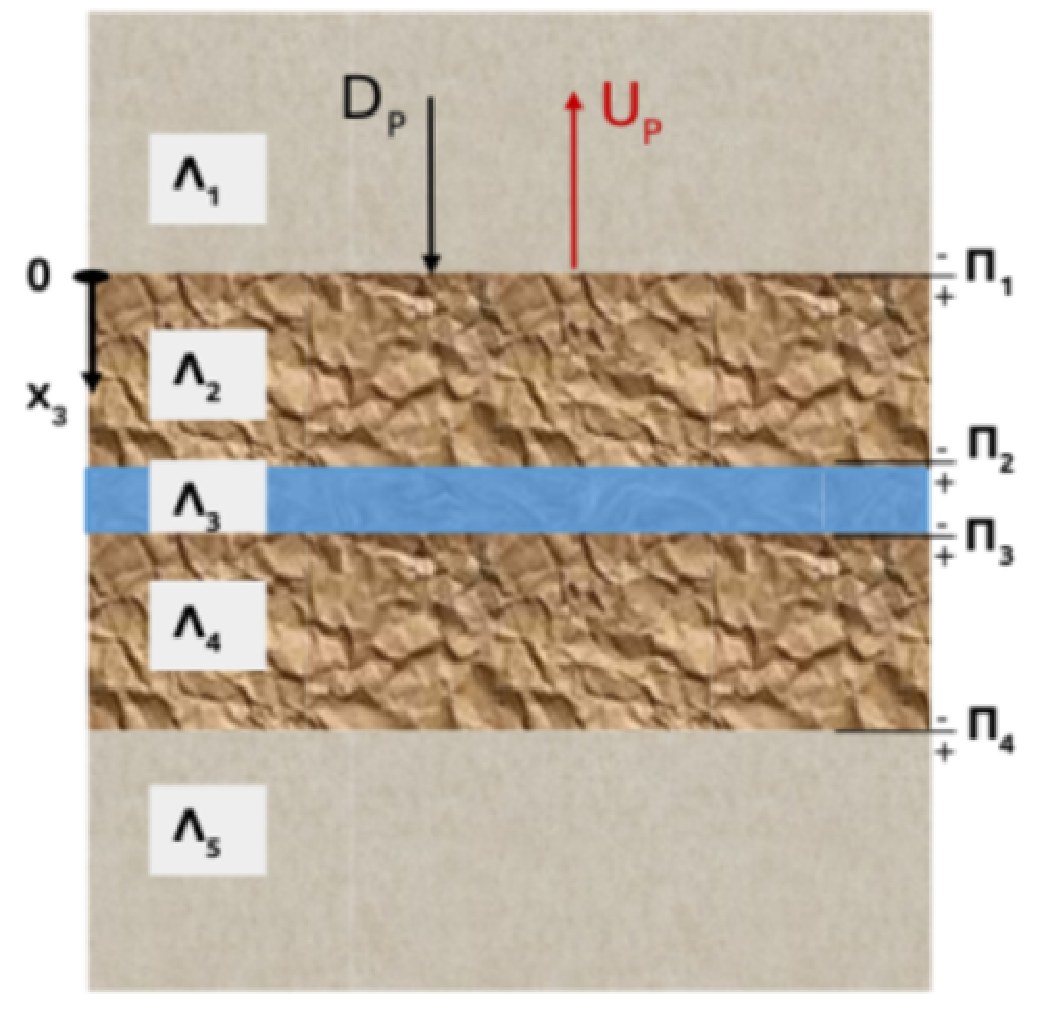
\includegraphics[width= 46mm, height=51mm]{./Figure1.pdf}
\caption{ Layered model considered for both the elastic-poroelastic  and purely elastic analyses. $D_P$ and $U_P$ are the downgoing and upgoing P-waves, respectively. $\Lambda_1$ and $\Lambda_5$ are half-spaces representing the elastic impermeable background; $\Lambda_3$ is the thin layer representing the  fracture, and $\Lambda_2$ and $\Lambda_4$ are the layers representing the DZ. For the elastic-poroelastic case, the fracture and DZ layers are poroelastic, while for the purely elastic case, all media are elastic. }
\label{fig:1}
\end{figure}

We assume a normally incident P-wave striking at the background-DZ interface $\Pi_1$. 
Then, 
our objective is to find the corresponding PP reflection coefficients $R_{PP}$ for both the elastic-poroelastic and purely elastic case, respectively. 
We compute the corresponding reflection coefficients at the DZ-background interface because it quantifies the amplitude of the reflected signal from the DZ-fracture system that could be recorded in a seismogram.
For this computation, we formulate the poroelastic and elastic wave equations in the space-frequency domain, assuming that the  medium is isotropic. To formulate the poroelastic wave equation,  we let $\bm{u}^s =\bm{u}^s( \bm{x}, \omega)$ and $\bm{w} =\bm{w}( \bm{x}, \omega)$  be the solid displacement vector and the relative fluid displacement vector, respectively, for any position $\bm{x}$ and angular frequency $\omega$. Moreover, we let $\bm {\sigma}$, and $p_f$ be the  
total stress
tensor and pore fluid pressure, respectively, which act upon the poroelastic medium. Then, we  express the corresponding equations of motion as \cite{Biot1962}:
\begin{linenomath*}
\begin{equation}\label{Eq.1}
\begin{split}
& -\,\omega^2  \, \rho_b  \, \bm{u}^s -  \,\omega^2 \, \rho_f \, \bm{w}= \nabla . \, \bm{\sigma}, \\
& -\,\omega^2  \, \rho_f \, \bm{u}^s - \omega^2 g(\omega) \, \, \bm{w} + i \, \omega \, b(\omega) \, \bm{w} = - \nabla \, p_f.
\end{split}
\end{equation}
\end{linenomath*}
The constitutive equations are:
\begin{linenomath*}
\begin{equation}\label{Eq.2}
\begin{split}
& \bm{\sigma} = \mu \,  \left( \nabla \,\bm{u}^s + {\nabla  \bm{u}^s}^T  \right) +  \left( \lambda \, \nabla . \, \bm{u}^s\, + \alpha \,M \, \nabla . \, \bm{w} \right) \bm{I}, \\
&p_f=- \alpha \, M \, \nabla . \, \bm{u}^s - M \, \nabla . \, \bm{w},  \end{split}
\end{equation}
\end{linenomath*}
where $\rho_b$ and $\rho_f$ are the bulk density of the saturated porous medium and the density of the pore fluid, respectively, $\mu$ is the frame shear modulus, $\phi$ is the porosity, $\bm{I}$ is the identity matrix, $i$ is the imaginary unit, $\lambda$ is the undrained Lamé modulus, $\alpha$ is the Biot-Willis effective stress coefficient, $M$ is the Biot's fluid storage modulus, and $g(\omega)$ and $b(\omega)$ are the mass coupling and viscous coefficients, respectively. The required rock physical properties are calculated as follows \cite<e.g.,>{Barbosa2016}:

\begin{linenomath*}
\begin{equation}\label{Eq.3}
\begin{split}
& \rho_b =(1-\phi)\rho_s + \phi \rho_f, \\
& \lambda= K_m - \frac{2}{3} \mu + \alpha^2 M, \\
& \alpha =1-\frac{K_m}{K_s},\\
& M  =\left( \frac{\alpha-\phi}{K_s} +\frac{\phi}{K_f} \right)^{-1}, \\
& g(\omega) =  \frac{1}{\omega} \Im \left( \frac{\eta}{\kappa_d(\omega)} \right),\\
& b(\omega) = \Re\left( \frac{\eta}{\kappa_d(\omega)} \right),
\end{split}
\end{equation}
\end{linenomath*}
where $\rho_s$ is the density of the solid grains, $K_m$, $K_s$, and $K_f$ are the bulk moduli of the drained solid frame, the solid grains, and the pore fluid, respectively. Additionally, $\eta$ is the viscosity of the pore fluid and $\kappa_d(\omega)$ is the dynamic permeability of the porous rock, which can be expressed as \cite{Johnson1987}:
\begin{linenomath*}
\begin{equation}\label{Eq.4}
    \kappa_d(\omega)=\kappa \left(\sqrt{1 + \frac{4 i \omega}{n_j \omega_B} }+ \frac{i \omega}{\omega_B}   \right) ^{-1}.
\end{equation}
\end{linenomath*}
Here, $\kappa$ is the static permeability of the porous medium, $\omega_B$ is  Biot's angular frequency, which can be expressed as:
\begin{linenomath*}
\begin{equation}\label{Eq.5}
  \omega_B = \frac{\eta \phi}{\rho_f \kappa S},
\end{equation}
\end{linenomath*}
where $S$ is the tortuosity of the pore space. Finally, $n_j$ is a parameter that  can be expressed as \cite{Johnson1987}:
\begin{linenomath*}
\begin{equation}\label{Eq.5.1}
  n_j = \frac{\phi \Lambda^2}{\kappa S},
\end{equation}
\end{linenomath*}
where $\Lambda$ is a parameter proportional to the pore-volume-to-surface ratio and has units of length \cite{Johnson1987}. According to numerical and experimental studies \cite<e.g.,>{Charlaix1988, Sheng1988, Smeulders1992}, $n_j$ = 8 is a reasonable approximation for most porous media and hence, we use this value in the following. In this context, it is, however, important to remark that the prevailing range of $n_j$ for fractured porous media remains, as of today, unexplored.
In spite of this uncertainty, it is expected that variations in $n_j$ will produce negligible changes on the predicted dynamic permeability $\kappa_d (\omega)$, since its decay is proportional to $\sqrt{2/n_j}$ \cite{Pride2003}. Most importantly, $n_j$ impacts the behavior of $\kappa_d (\omega)$ only at sufficiently high frequencies, that is $\omega$ $>>$ $\omega_B$. As explained later in section 2.3, this work focuses on the poroelastic response at lower frequencies, that is $\omega$ $<<$ $\omega_B$, where $\kappa_d (\omega)$ approaches the value of the static permeability $\kappa$.

To formulate the elastic wave equation, we let $\bm{u}^e=\bm{u}^e (\bm{x},\omega)$ be the displacement vector for any position $\bm{x}$ in the elastic medium and angular frequency $\omega$. We also let $\bm{\sigma}^e$ be the stress tensor field acting upon the medium. Then, we express the corresponding equations of motion as:
\begin{linenomath*}
\begin{equation}\label{Eq.6}
- \, \rho_b \,\omega^2 \, \bm{u}^e = \nabla . \, \bm{\sigma}^e.
\end{equation}
\end{linenomath*}
The associated constitutive equation is given by: 
\begin{linenomath*}
\begin{equation}\label{Eq.7}
\bm{\sigma}^e = \mu \,  \left( \nabla \, \bm{u}^e + {\nabla  \bm{u}^e}^T  \right) + \lambda \,  \nabla . \, \bm{u}^e\,\, \bm{I}.
\end{equation}
\end{linenomath*}
 

\subsection{Solution for displacements and PP reflection coefficients}
\subsubsection{Total displacements}
We assume that an incident P-wave propagates downwards, in the $\bm{\hat x_3}$ direction (Figure \ref{fig:1}), and strikes the interface $\Pi_1$ at normal incidence. 
Under this condition, for the elastic-poroelastict model, the propagating modes present in the elastic half spaces $\Lambda_1$ and $\Lambda_5$ are P-waves, while in the poroelastic layers $\Lambda_2$, $\Lambda_3$ and $\Lambda_4$, both fast ($P_1$) and slow ($P_2$) P-waves are present. For the purely elastic model,  only P-waves are present throughtout the model.
Note as well that the only non-zero component of the displacement vectors is in $\bm{\hat x_3}$.
Then, to find the total displacements at each medium $\Lambda_m$, with $m$ = $1,..,5$, we sum the corresponding displacements produced by the waves traveling in the given medium $\Lambda_m$.

For the elastic-poroelastic model, we need to consider two types of media: elastic and poroelastic. We let $u_n^{\epsilon}$ be the total displacement for each elastic medium $n$, where  $n$ refers to the upper half-space $\Lambda_1$  and  lower half-space $\Lambda_5$, respectively. When $n$ corresponds to $\Lambda_1$ the expression for $u_n^{\epsilon}$ is given by:
\begin{linenomath*}
\begin{equation}\label{Eq.8}
u_n^{\epsilon} =  u_{n\,{D_P}}^{\epsilon}  + u_{n\,{U_P}}^{\epsilon} , \; \; 
\end{equation}
\end{linenomath*}
where $D$ and $U$ refer to the downgoing and upgoing waves, respectively, and the subscript $P$ refers to the P-wave. Since in the lower half-space $\Lambda_5$ there are no upgoing-waves, $u_n^{\epsilon}$ simplifies to:
\begin{linenomath*}
\begin{equation}\label{Eq.8.1}
u_n^{\epsilon} = u_{n\,{D_P}}^{\epsilon} , \; \; 
\end{equation}
\end{linenomath*}

For each poro\-elastic layer $d$, with $d$ = $\Lambda_2$, $\Lambda_3$, and $\Lambda_4$, we let
$u{_d^s}$ be the total solid displacement and $w_d$ the total relative fluid displacement, respectively. Then, we express these total displacements as:
\begin{linenomath*}
\begin{equation}\label{Eq.9}
u_d^s =  \sum_q u_{d \,q}^s ,   \qquad
w_d = \sum_q  w_{d \,q}  \;,
\end{equation}
\end{linenomath*}
with $q=D_{P_1},D_{P_2}, U_{P_1},U_{P_2}$, where the subscripts $P_1$ and $P_2$ indicate the associated fast and slow P-waves, respectively.

On the other hand, for the purely elastic model, we let $u_n^e$ be the elastic displacement component for each elastic medium $n$ = $\Lambda_1,.., \Lambda_5$. The expression for the total displacement $u_n^e$  for each medium $n$, except $\Lambda_5$, is then given by equation \eqref{Eq.8}. For $\Lambda_5$, the total displacement $u_n^e$ is given by equation \eqref{Eq.8.1}. We remark that the respective terms in equations \eqref{Eq.8} and \eqref{Eq.8.1} are replaced by $u_n^e$ and $u_{n\,j}^e$, where $j$ can be either $D_P$ or $U_P$.

\subsubsection{Solution for displacements}
For the elastic-poroelastic model, we express
the corresponding solution $u_{n\,j}^\epsilon$ for each elastic medium $n$ = $\Lambda_1$ and $\Lambda_5$, with $j$ = $D_P$ or $U_P$, as:
\begin{linenomath*}
\begin{equation}\label{Eq.10}
u_{n\,j}^{\epsilon} = E_{n \,j}^{\epsilon} \;\exp[ \pm\; i \; k_{n}^{\epsilon} \; x_3 ]\,,
\end{equation}
\end{linenomath*}
where $E_{n \,j}^{\epsilon}$ is the amplitude of the corresponding elastic displacement and $x_3$ is the position. Negative and positive signs in the exponential correspond to downgoing and upgoing waves, respectively. $ k_{n}^{\epsilon}$ is the elastic scalar wave\-number for the P-wave in medium $n$, calculated as $ k_{n}^\epsilon$ = $\omega / V_P^n$, where $V_P^n$ is the P-wave velocity of medium $n$. 
The corresponding $V_P^n$ is:
\begin{linenomath*}
\begin{equation}\label{Eq.12}
V_P^n = \sqrt{\frac{\lambda^n +  2\, \mu^n}{\rho_b^n}} .
\end{equation}
\end{linenomath*}
Here, $\lambda$ and $\rho_b$ are the undrained Lamé modulus and the bulk density, respectively (equation \eqref{Eq.3}).
For the poro\-elastic layers  $d$ = $\Lambda_2$, $\Lambda_3$, and $\Lambda_4$, we express the solution for the solid and relative fluid displacement $u_{d\,q}^s$ and $w_{d\, q}$ as:
\begin{linenomath*}
\begin{equation}\label{Eq.11}
\begin{split}
& u_{d\,q}^s = S_{d\, q}\;\exp[ \pm \; i \; k_{d \,j} \; x_3 ] \, ,\\
& w_{d \,q} = W_{d\,q}\;\exp[\pm \; i\;  k_{d\,j} \;x_3 ] \, ,
\end{split}
\end{equation}
\end{linenomath*}
where $ S_{d\, q}$ and $W_{p\,q}$
are the amplitudes of the solid and relative fluid displacements, respectively. Additionally, 
$ k_{d\,j}$ is the poroelastic scalar wave\-number for the wave $j$ in layer $d$, with $j=P_1$ when $q=D_{P_1},U_{P_1}$ and $j=P_2$ when $q=D_{P_2},U_{P_2}$. Please note that the scalar wave\-number $ k_{d\,j}$ is complex-valued, frequency-dependent and its real part is associated with the phase velocity. To obtain
$ k_{d\,j}$, we follow the procedure employed by \citeA{Barbosa2016}.

For the purely elastic model, the expression for the solution of $u_{n\,j}^e$ for each elastic medium $n$, $n$ = $\Lambda_1,.., \Lambda_5$, is the same as the one stated in equation \eqref{Eq.10}, after replacing the corresponding terms by $E_{n \,j}^e$ and $k_{n}^e$.

\subsubsection{PP reflection coefficient}

We aim to find the PP reflection coefficients $R_{PP}$ = $R_{PP}^\epsilon$ and $R_{PP}$ = $R_{PP}^e$  at the interface  $\Pi_1$ of the half-space $\Lambda_1$ in both the elastic-poroelastic and purely elastic models, respectively (Figure \ref{fig:1}). Without loss of generality, we assume that the amplitude of the incident P-wave is one:
$ \tensor*[]{E}{*^\epsilon_{\text{\tiny $\Lambda_1$}}_{ \text{\tiny $D_P$}}}$ =  $\tensor*[]{E}{*^e_{\text{\tiny $\Lambda_1$}}_{\text{\tiny $D_P$}}}$ = $1$.
Then, we seek to find the amplitudes of the reflected P-waves at the interface $\Pi_1$ of the upper half-space $\Lambda_1$: $R_{PP}^\epsilon$ = $ \tensor*[]{E}{*^\epsilon_{\text{\tiny $\Lambda_1$}}_{ \text{\tiny $U_P$}}}$ and 
$R_{PP}^e$ = $\tensor*[]{E}{*^e_{\text{\tiny $\Lambda_1$}}_{\text{\tiny $U_P$}}}$.
To this end,
we assemble sets of linear equations, which we find by imposing suitable continuity conditions at the corresponding media interfaces.

For the elastic-poroelastic model, we distinguish two types of interfaces: elastic-poroelastic and purely poroelastic ones. At the elastic-poroelastic interfaces $\Pi_q$, for  $q=1,4$,
we impose continuity of solid displacements and tractions and we set to zero the relative fluid displacements, respectively \cite{Deresiewicz1963}: 
\begin{linenomath*}
\begin{equation}\label{Eq.13}
\begin{split}
&  \left. \left(  u_n^\epsilon -  u_d^s \right) \right \rvert_{\Pi_q} = 0 \,, \\
&  \left. \left(  t_n^\epsilon -  t_d \right) \right \rvert_{\Pi_q} = 0 \,,\\
& \left.  w_d^s \right \rvert_{\Pi_q} = 0 \,.
\end{split}
\end{equation}
\end{linenomath*}
For $q=1$, the corresponding media are $n=\Lambda_1$ and $d=\Lambda_2$; for $q=4$, they are $n=\Lambda_5$ and $d=\Lambda_4$.
We calculate the traction component $t_n^\epsilon$ as $t_n^\epsilon$ = $ ({\bm{\sigma}^\epsilon} \,^{\bm{.}} \,\bm{\hat x_3}) \, ^{\bm{.}} \, \bm{\hat x_3}$. Then, using equation (\ref{Eq.7}) to replace $\bm{\sigma}^\epsilon$, we express $t_n^\epsilon$ as:
\begin{linenomath*}
\begin{equation}\label{Eq.14}
t_n^\epsilon =(\lambda^n + 2 \mu^n)\,  \left( \, u_n^{\epsilon} \, \right)_{,3} \,,
\end{equation}
\end{linenomath*}
where  $(^.)_{,3}$ = $\partial (^.)/ \partial{x_3}$. 
Similarly,  we calculate the traction component $t_d$ as $t_d$ = $(\bm{\sigma} \, ^{\bm{.}} \, \bm{\hat x_3}) ^{\bm{.}} \, \bm{\hat x_3}$ and, using equation (\ref{Eq.2}) to replace  $\bm{\sigma}$, we obtain $t_d$:
\begin{linenomath*}
\begin{equation}\label{Eq.15}
t_d =  (\lambda^d + 2 \mu^d)\,  \left( \, u_d ^s \, \right)_{,3}\; + \alpha^d M^d \,  \left( \, w_d \right)_{,3} \,.
\end{equation}
\end{linenomath*}

At the purely poroelastic interfaces $\Pi_q$ with $q=2,3$, we impose the continuity of solid displacements, relative fluid displacements, tractions, and fluid pressures, respectively \cite{Deresiewicz1963}:
\begin{linenomath*}
\begin{equation}\label{Eq.16}
\begin{split}
&  \left. \left( u_d^s -  u_{(d+1)}^s \right) \right \rvert_{\Pi_q} = 0 \,, \\
&  \left. \left(  w_d -  w_{(d+1)} \right) \right \rvert_{\Pi_q} = 0 \,, \\
& \left . \left(  t_d  - t_{(d+1)}  \right) \right \rvert_{\Pi_q}= 0 \,,\\
&  \left. \left(  p_{f\,d} -  p_{f\, (d+1)} \right) \right \rvert_{\Pi_q} = 0 \,.
\end{split}
\end{equation}
\end{linenomath*}
Here, $d$ = $\Lambda_q$ and ($d+1$) = $\Lambda_{(q+1)}$. Moreover, we calculate $t_d$ and $t_{(d+1)}$ using equation (\ref{Eq.15}). 
Additionally, using equation (\ref{Eq.2}), we evaluate the pore fluid pressure:
\begin{linenomath*}
\begin{equation}\label{Eq.17}
p_{f \, d} = - \alpha^d M^d\,  \left( \, u_d^{s} \, \right)_{,3}\; - M^d \,  \left( \, w_d \right)_{,3} \, .
\end{equation}
\end{linenomath*}
To complete the system of equations, we express the relative fluid displacement in terms of the solid displacement through
 $\tensor []{\gamma}{_d_{\,j}}=\tensor*[]{W}{_d_{\, j}}/\tensor*[]{S}{_d_{\, j}}$ where $j=P_1, P_2$. This ratio can be  obtained from the properties of the porous medium \cite{Barbosa2016}.
 
For the elastic model, we obtain the corresponding system of equations by imposing the continuity of displacements and tractions  at each medium interface $\Pi_q$ with $q=1,..,4$, respectively:
\begin{linenomath*}
\begin{equation}\label{Eq.18}
\begin{split}
&  \left. \left(  u_n^e -  u_{(n+1)}^e \right) \right \rvert_{\Pi_q} = 0 \,, \\
&  \left. \left( t_n^e  - t_{(n+1)}^e  \right) \right \rvert_{\Pi_q} = 0 \,.
\end{split}
\end{equation}
\end{linenomath*}
Here, $n$ = $\Lambda_q$ and ($n+1$) = $\Lambda_{(q+1)}$. We calculate $t_n^e$  and $t_{(n+1)}^e$ using equation (\ref{Eq.14}) after replacing the corresponding displacement term by $u_n^e$.

\subsection{FPD frequency regimes}
When seismic waves propagate through heterogeneous materials, pore fluid pressure perturbations arise between regions of differing compresibilities. These pressure gradients are equilibrated through FPD, which, depending on the size of the underlying heterogeneities, prevails at different scales. Our analysis focuses on the mesoscopic scale, which refers to those heterogeneities that are larger than the pore size but much smaller than the wavelength of the propagating wave. For the case of compliant fractures embedded in a much stiffer DZ, the compressi\-bility contrast allows seismic waves to induce strong fluid pressure gradients and  associated fluid flow.

On the other hand, it is important to notice that FPD prevails at frequencies much lower than Biot's characteristic frequency of the medium: $f$ $\ll$ $f_B$, with $f_B$ =$\omega_B/(2 \pi)$ (equation \ref{Eq.5}). At these sufficiently low frequencies, the fluid flow within the pores is viscous-dominated,  provided that the thickness of the viscous boundary layer remains greater than the characteristic pore size \cite{Johnson1987}. Under this condition, the  imaginary part of the dynamic permeability $k_d (\omega)$ becomes negligible (equation \ref{Eq.4}).
Moreover, in the low-frequency limit, $k_d (\omega)$  becomes real-valued and frequ\-ency\--independent and equal to the static permeability $\kappa$: $ \lim \limits_{\omega \to 0}k_d (\omega)$ = $\kappa$. If we additionally constrain the analysis of Biot's equations to the quasi-static case, it can be shown that the behavior of the slow P-wave is described by a pressure diffusion equation with diffusion coefficient $D$ \cite{Chandler1981}: 
\begin{linenomath*}
\begin{equation}\label{Eq.19}
D = \frac{\kappa}{\eta} \frac{M H_d}{H},
\end{equation}
\end{linenomath*}
where the drained and undrained plane-wave moduli $H_d$ and $H$ can be calculated as $H_d= K_m + 4/3 \,\mu$ and $H = \lambda + 2 \mu$, respectively. Moreover, we let  $L_d$ be the characteristic diffusion length \cite{Norris1993}: 
\begin{linenomath*}
\begin{equation}\label{Eq.20}
L_d = \sqrt{\frac{D}{\omega}}.
\end{equation}
\end{linenomath*}
As the frequency varies, distinct FPD regimes can be identified according to the relative magnitudes between the scale of a heterogeneity and its characteristic diffusion length. For the case of a fracture surrounded by DZ, the relevant scales are their respective thicknesses. For simplicity, let us assume that the thickness of the fracture $h^c$ is negligible compared to that of the DZ and that its diffusion coefficient (equation \eqref{Eq.19}) is very high.
In this context, we have $h^c \ll L_d^c$ for the frequency range of interest. Here, the superscript $c$ refers to the fracture. Conversely, if we consider that the DZ thickness is much larger than that of the fracture but its permeability is much lower, then we expect that the relationship between DZ thickness $h^z$ and its characteristic diffusion length $L_d^z$  varies from $h^z\ll L_d^z$  to $h^z\gg L_d^z$ as frequency increases.
Thus, for the fracture-DZ poroelastic system, we can regard the thickness of the DZ $h^z$ as the relevant mesoscopic heterogeneity scale controlling FPD. Under this perspective, we  distinguish the following two end-member regimes for FPD: relaxed and unrelaxed. The relaxed state occurs at sufficiently low  frequencies, at which the diffusion length $L_d^z$ is larger than the thickness of the DZ $h^z$.
Thus, there is enough time for the pressure between the fracture and DZ layers to equilibrate. Conversely, the unrelaxed state occurs at sufficiently high frequencies, at which the diffusion length $L_d^z$ is very small compared to thickness of the DZ $h^z$ and, consequently, there is no time for FPD to take place, and the medium behaves as hydraullically isolated. A transition zone exists at intermediate frequencies, at which the diffusion lengths are of comparable size to that of the thickness of the DZ $h^z$. This zone is characterized by a transition frequency $f_c = \omega_c /2 \pi$, which can be estimated as \cite{Brajanovski2006, Muller2006}: 
\begin{linenomath*}
\begin{equation}\label{Eq.21}
   w_c \approx  \frac{9}{2} \frac{D^z}{(h^z)^2}.
\end{equation}
\end{linenomath*}
We remark that \citeA{Brajanovski2006} and \citeA{Muller2006} have also pointed to the existence of a second characteristic frequency that, depending on the DZ and fracture properties, could be visible in the transition zone. However, 
for the rock and fluid properties we are using in this work, this second characteristic frequency is not visible.

In this work, we consider an open fracture whose permeability is several orders of magnitude greater than the DZ. Then, it is expected that $f_B^c$ $<<$ $f_B^z$, meaning that FPD within the fracture is limited to much lower frequencies than for the DZ. Particularly, for frequencies greater than $f_B^c$ but lower than $f_B^z$, FPD does no longer take place within the fracture since fluid flow becomes inertial-dominated, but FPD is still present within the DZ.  We remark that, the proposed solutions for amplitude displacements, as expressed in equation (\ref{Eq.10}), account for both fluid flow regimes, viscous- and inertial-dominated, since they include the dynamic permeability (equation \ref{Eq.4}) in the calculation of the poroelastic wavenumbers  of the fracture and DZ. Therefore,
within this frequency band, pressure equilibration will take place under two different flow regimes. Nonetheless, due to the greater thickness and lower permeability of the DZ, it is expected that the viscous-dominated fluid flow regime in this region controls the reflectivity response of the DZ-fracture system. 
Moreover, hereinafter we use the terms low- and high-frequency limits  within the FPD context. Meaning that, they signify the relaxed and unrelaxed FPD regimes, respectively.

\subsection{Normal fracture compliance}
Fracture compliance defines the mechanical behavior of a fracture. The more compliant a fracture is, the easier it undergoes deformation and the higher is its seismic reflectivity since the mechanical contrast with the background increases. For the case of FPD effects caused by a normally incident P-wave, our interest focuses on normal fracture compliance. For the fracture-DZ poroelastic system, FPD  allows fluid to flow from the more compliant fracture to the stiffer DZ during half of a wave cycle, which, in turn, decreases the stiffening effect of the fracture fluid, thus 
increasing the normal compliance of the fracture and its reflectivity.
However, the extent to which normal fracture compliance and its reflectivity increase
is controlled by the FPD regimes. Normal compliance is maximal, associated with a maximal increase of reflectivity, when FPD is in its relaxed state, that is, when the fracture fluid is allowed to exit until the pressure fully equilibrates. In contrast,  normal fracture compliance is lowest, with no reflectivity enhancement during the unrelaxed FPD regime, in which the fracture behaves as hydraulically isolated. Intermediate values of normal fracture compliance are expected as FPD transitions from its relaxed to its unrelaxed regime.

We calculate the normal fracture compliance  $Z_N^e$ for the elastic fracture represented as a thin layer using the definition introduced by \citeA{schoenberg1980elastic}. Then, extending this concept to a poroelastic framework in a similar way to \citeA{Rubino2015a}, we also calculate the normal fracture compliance $Z_N^p$ for the poroelastic fracture also represented as a thin layer:
\begin{linenomath*}
\begin{equation}\label{Eq.22}
\begin{split}
& Z_N^e =  \frac{ \left.u_{n}^e \right \rvert_{\Pi_3} - \left.u_{n}^e \right \rvert_{\Pi_2}}{\bar t^{\,e}_n},  \quad \text{with} \quad
\bar t^{e}_{n} = \frac{ \left.t^{e}_{n} \right \rvert_{\Pi_2}+ \left.t^{e}_n \right \rvert_{\Pi_3}}{2}\; , \\
& Z_N^p =  \frac{ \left.u_{d }^s \right \rvert_{\Pi_3} - \left.u_{d}^s \right \rvert_{\Pi_2}}{\bar t_d},  \quad \text{with} \quad
\bar t_{d} = \frac{ \left.t_{d} \right \rvert_{\Pi_2}+ \left.t_{d} \right \rvert_{\Pi_3}}{2} \;,
\end{split}
\end{equation} 
\end{linenomath*}
with $n$ = $d$  = $\Lambda_3$.
Here, we do not imply that it is seismically equivalent to represent the 1D poroelastic DZ-fracture system by a slip interface characterized by a  poroelastic normal compliance equal to $Z_N^p$. But the main purpose of calculating $Z_N^p$ is to show the effect of FPD on normal fracture compliance. We refer the reader to the first paragraph of the discussion section for further details.

On the other hand, we express the normal fracture compliance in the relaxed and unrelaxed FPD regimes, $Z_N^o$ and $Z_N^u$, as \cite{Rubino2015a}:
\begin{linenomath*}
\begin{equation} \label{Eq.23}
\begin{split}
 & Z_N^o= Z_N^u + \frac{2 B^{c} \left(B^c-B^z \right)}{ \frac{2 B^c}{\alpha^z Z_N^d} + \frac{M^z(1-\alpha^z B^{z})}{h^z} }\,,\\
 & Z_N^u= \frac{h^{c}}{H^{c}}\,.
\end{split}
\end{equation}
\end{linenomath*}

Here, $B$ is the Skempton coefficient, which can be written as $B=\alpha M/H$. 
Note that, $Z_N^o$ and $Z_N^u$ can also be designated as the low- and high-frequency limits of fracture compliance, respectively. In the context of FPD,
$Z_N^o$ and $Z_N^u$ are the maximum and minimum values that the normal compliance of a fracture can assume for a given set of rock and fluid properties. In particular, the high frequency-limit of normal fracture compliance $Z_N^u$ corresponds to the elastic behavior of the fracture since at sufficiently high frequencies there is no time for FPD to take place and the fracture behaves as hydraulically isolated. This, in turn, impedes the outflow of the stiffening fluid from the fracture causing its compliance to decrease to this minimum value.
Moreover, as detailed by equation \ref{Eq.23}, the high-frequency limit of fracture compliance  $Z_N^u$ only depends on the fracture physical properties.
In this work, we use the ratio $Z_N^o/Z_N^u$ as a measure of the maximum increase of normal fracture compliance due to FPD with respect to its elastic limit. We remark that
\citeA{Rubino2015a} find the expressions for $Z_N^o$ and $Z_N^u$ by considering a 1D periodic system consisting of a relatively thick horizontal layer alternating with a thinner layer representing a fracture. They assume a representative elementary volume (REV) comprised of the fracture layer as well as the two embedding layers with half of their thicknesses. 
They also assume a no-flow condition at the  upper and lower boundaries of the REV, which holds for the entire system given the symmetry of the problem and its infinite nature. For  the fracture-DZ poroelastic system enclosed within elastic half-spaces considered in this work, periodicity is no longer required to ensure the no flow condition since this is, in fact imposed, by the zero relative fluid displacement boundary condition at the the interfaces between the poroelastic DZ and elastic half-spaces representing the impermeable background (equation \ref{Eq.13}). Thus, the expressions in equation (\ref{Eq.23}) are applicable for our problem when we consider the entire thickness of the DZ.
%*****************
%RESULTS
%*****************
\section{Results}

In  this section, we present results of frequency-dependent reflectivity and normal fracture compliance for the elastic-poroelastic and elastic models. 
%For the poroelastic model,
We analyze the effects of variations of rock properties of the DZ and of the fracture, as well as of the pore fluid, on the reflectivity and on the normal compliance.
We remark that for high-enough frequencies, the results from the elastic-poroelastic models should converge to those obtained from the corresponding elastic models. This convergence is expected because in the high-frequency limit the unrelaxed FPD regime prevails. This effect, as previously explained, prevents fluid exchange between the poroelastic fracture and the DZ and, which as a consequence, causes them to behave elastically.
For these examples, we use rock and fluid properties from Table \ref{fig:1}, which
shows the reference values of the rock and fluid properties for the poroelastic thin layer representing the fracture and the associated DZ layers. Most of these values are adopted from  \citeA{Barbosa2016} and \citeA{Barbosa2019}, with rock properties emulating those of a crystalline lithology. Fracture bulk and shear moduli, $K_{m}^c$ and $\mu^c$, are estimated using the formulae proposed by \citeA{Nakagawa2007}:
\begin{linenomath*}
\begin{equation} \label{Eq.24}
Z_T^d=h^c/\mu^c ; \qquad Z_N^d=h^c/(K_{m}^c + 4/3 \, \mu^c).
\end{equation}
\end{linenomath*}
For the drained tangential $Z_T^d$ and normal $Z_N^d$ compliances, we assume values of  \num{5e-10} m/Pa and \num{1.5e-10} m/Pa, respectively. The magnitude of these values ($\sim \num {e-10}$ m/Pa) corresponds to a fracture of around a hundred meters long \cite{Hobday2012}.
For the elastic media, comprised by the elastic fracture, DZ and background, we compute the corresponding elastic moduli using Gassmann's equations \cite{Gassmann1951} and we take the required rock and fluid properties from Table \ref{table:1}. For calculations corresponding to the elastic background and DZ, we take the necessary rock properties from the ones listed for the DZ and, in a similar way, for the elastic fracture, we take the required properties from the poroelastic fracture. We indicate that, for the rock and fluid properties listed in Table \ref{table:1}, Biot's frequencies for the poroelastic DZ and the fracture are \num{8.1e3} Hz and \num{1.2e3} Hz, respectively.

\begin{table}[!ht]
  \caption{Reference values of the physical properties for the DZ, fracture, and pore fluid.}
\begin{center}
  \begin{tabular}{ | l | c | c| }
    \hline
    Property & DZ & Fracture \\ \hline
    Grain bulk modulus $K_s$ (\rm{GPa}) & 37 & 37 \\ 
    Grain density $\rho_s$ ($\rm{Kg/m^3}$) & 2730 & 2730 \\
    Porosity $\phi$ & 0.015 & 0.8 \\
    Frame bulk modulus $K_m$ (\rm{GPa}) & 33 & 0.004\\ 
    Frame shear modulus $\mu$ (\rm{GPa}) & 29 & 0.002 \\
    Thickness $h$ (m) & 0.2 & 0.001\\ 
    Permeability $\kappa$ (D) & 0.1 & 100\\
    Tortuosity $S$ & 3 & 1\\
    Fluid density $\rho_f$ ($\rm{Kg/m^3}$) & 1000 & 1000\\
    Fluid bulk modulus $K_f$ (\rm{GPa}) & 2.25 & 2.25\\
    Fluid viscosity $\eta$ (\rm{Pa.s})& 0.001 & 0.001\\
    %Pore geometry parameter $n_j$ & 8 & 8\\
    \hline
  \end{tabular}
  \label{table:1}
\end{center}
\end{table}

Notice that, unless stated otherwise, we use the same rock physical properties for the DZ and the background, except for the permeability, to simplify the interpretation of results, since we want to emphasize the FPD effects induced by the presence of the DZ surrounding a fracture. 
Furthermore, please note that we do not include intrinsic attenuation effects in the DZ, although they are expected to take place due to the presence of macro- and micro-fractures. Nonetheless, we consider that these simplifications are justified since they aim to highlight FPD effects on the reflectivity response.


\subsection{ Effect of permeability of the DZ}
In the following example, we show the effect of different DZ permeabilities on reflectivity and  normal fracture compliance. As previously outlined, it is the permeability of the DZ that allows for the hydraulic communication with the adjacent fracture for FPD to take place.

Figure \ref{fig:2} shows the absolute value of the normal-incidence reflection coefficient $|R_{PP}|$ versus frequency for the elastic and the elastic-poroelastic models considering different DZ permeabilities $\kappa^z$. These results show that there is a maximum increase of reflectivity for the elastic-poroelastic models of approximately one order-of magnitude when compared to the elastic results for frequencies lower than the respective transition frequencies $f_c$. This is a consequence of FPD prevailing between the DZ and the fracture, which allows for fluid release from the fracture as the pressure equilibrates during a half wave cycle. 
We observe that the role of the DZ permeability $\kappa^z$ is to control the transition frequency, at which reflectivity decreases towards its undrained values. Here, higher permeabilities shift this transition frequency towards higher values. This is expected given that the characteristic transition frequency $f_c$ is directly proportional to the permeability $\kappa^z$ (equations \ref{Eq.19} and \ref{Eq.21}). We also note that, for all elastic-poroelastic models, there is an upper limit for $|R_{PP}|$ regardless of the permeability $\kappa^z$. This is due to the fact that, irrespective of its permeability, the DZ provides a limited pore volume for FPD to occur in its relaxed state. We present a detailed analysis regarding this subject in the next subsection. Notice as well the presence of reverberations of $|R_{PP}|$ at high frequencies for a permeability of 1 D. For this permeability, the corresponding Biot's frequency in the DZ is $ \sim$ 800 Hz and at this frequency $P_2$ becomes a propagating wave. Then, multiples are expected within the poroelastic DZ layer when the wavelength of $P_2$ becomes smaller than the layer thickness. These multiples convert to upgoing $P_1$-waves at the background-DZ interface and interfere constructively and destructively with the reflected $P_1$ at this interface. Furthermore, at frequencies comparable to or larger than Biot's frequency, the relaxation mechanism is no longer controlled  by viscous diffusion but by inertial forces. In that case, equations (\ref{Eq.19}) to (\ref{Eq.21}), which assume a pressure diffusion mechanism, no longer apply.

\begin{figure}
\centering
        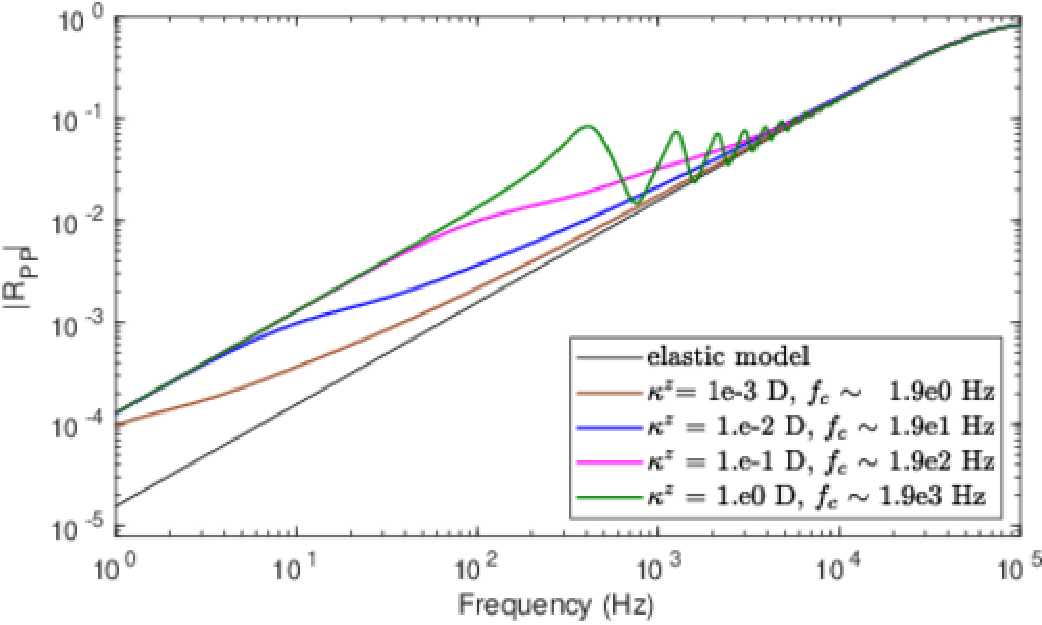
\includegraphics[width=80mm, height=50mm]{Figure2.pdf}
\caption {Absolute value of normal-incidence P-wave reflection coefficient $|R_{PP}|$ as a function of frequency for different DZ permeabilities $\kappa^z$.}
\label{fig:2}
\end{figure}

Figures \ref{fig:3}a and \ref{fig:3}b show the real and imaginary parts of the normal fracture compliance, respectively, as a function of frequency for different values of the DZ permeability 
$\kappa^z$. We use equation (\ref{Eq.22}) to calculate both the elastic normal fracture compliance $Z_N^e$ and the poroelastic normal fracture compliance $Z_N^p$, respectively. As expected, the elastic normal compliance $Z_N^e$ is constant for all frequencies and presents the lowest compliance value, thus, indicating the undrained limit. In contrast, the poroelastic normal compliance $Z_N^p$  becomes complex-valued and frequency-dependent as the FPD regime transitions from the relaxed  to the unrelaxed states. 
We point out that experimental support for the frequency-dependence of normal fracture compliance in poroelastic media has been provided by the work of \citeA{Nakagawa2013}. This study presents results of fracture stiffness (inverse of compliance) as a function of frequency for a fluid-saturated fracture, showing curves with similar trends as those in Figure \ref{fig:3}a.
Notice that at the high-frequency limit, the real part of all poroelastic normal compliances $Re[Z_N^p]$ (Figure \ref{fig:3}a) converges to the value of the elastic normal compliance $Z_N^e$. This is because, at this frequency limit, there is not enough time for FPD to take place and the fracture behaves as hydraulically isolated.
Regarding the behavior of normal fracture compliance at the low-frequency limit, Figure \ref{fig:3}a shows that,
at sufficiently low frequencies, the values of $Re[Z_N^p]$ are highest since the fracture experiences the maximum deformation while the maximum fluid exchange occurs between the DZ and the fracture. Nonetheless, there is an upper limit for $Re[Z_N^p]$ regardless of the DZ permeability, which is constrained by  the pore volume available in the DZ for FPD. 
In addition, using equation (\ref{Eq.23}), we obtain the fracture normal compliance for the low-frequency limit, $Z_N^o$ = \num{3.4e-12} m/Pa and the
high-frequency limit, $Z_N^u$ =  \num{3.6e-13}  m/Pa, respectively, which corresponds to a ratio $Z_N^o/Z_N^u$ equal to 9.45. 
To corroborate the accuracy of these results, we also estimate the average normal compliance for these frequency limits directly from the plots presented in Figure \ref{fig:3}a. To this end, we use the results from the curves with $k^z$ equal to \num{e-2} D and \num{e-1} D at a frequency of 1 Hz for the low-frequency limit and at a frequency of \num{4.5e4} Hz for the high-frequency limit. We perform the analysis with those two curves since they present both of the regimes relaxed and unrelaxed for the frequencies chosen. 
Although their compliances should be the same at these limits,  we can expect minor precision errors due to floating numbers used for the computations, thus we report the average of the compliances.
We obtain  \num{3.39e-12} m/Pa and \num{3.65e-13} m/Pa for the average compliances in the low- and high-frequency limits, respectively. Comparing these results with the ones obtained using equation (\ref{Eq.23}), we find that the errors are of the order of 1 \% or less.
Moreover, as remarked for Figure \ref{fig:2}, the DZ permeability controls the transition frequency towards the undrained normal compliance. The estimated values  for the respective transition frequencies $f_c$ are presented in Figure \ref{fig:2}. 
At this transition frequency, the magnitude of the imaginary part of fracture normal compliance has a peak (Figure \ref{fig:3}b), which indicates that maximum energy dissipation is taking place. This is the result of FPD occurring at a characteristic length $h^z$ that has a comparable size to that of the diffusion length $L_d^z$ (equation \eqref{Eq.20}).
Overall, these results indicate that FPD effects increase the normal fracture compliance as fluid exchange occurs between the fracture and the DZ, which, in turn, increases the reflectivity of the poroelastic fracture-DZ system. 


\begin{figure}
\centering
        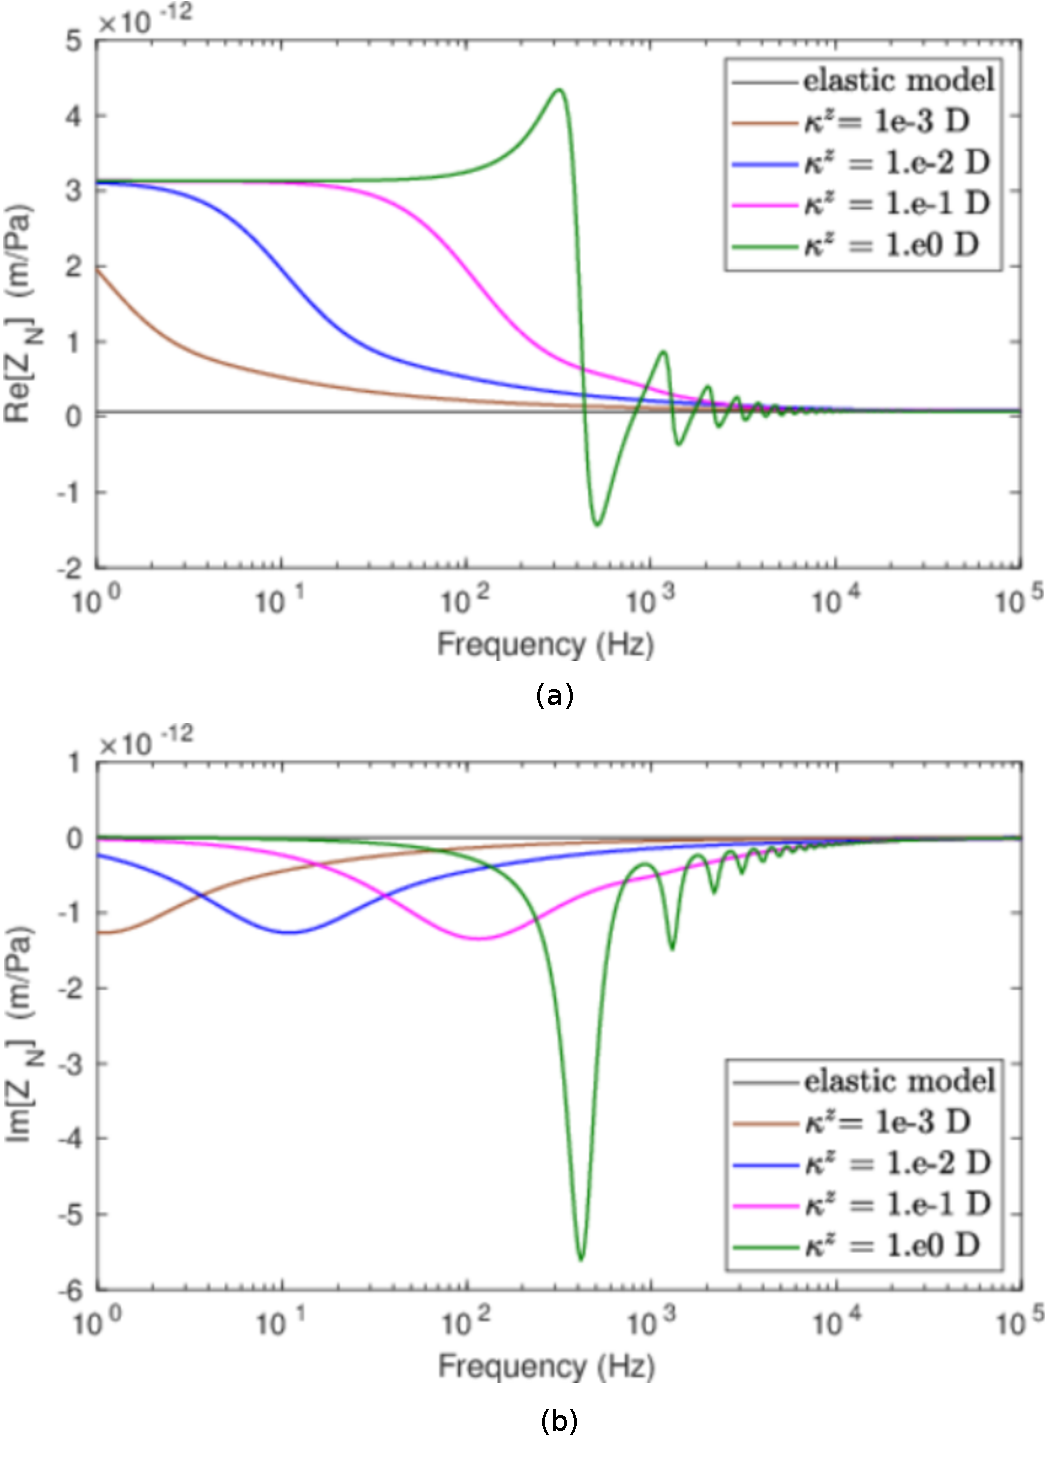
\includegraphics[width=85mm, height=110mm]{Figure3.pdf}
\caption {(a) Real and (b) imaginary parts of  normal fracture compliance $Z_N$ as functions of frequency for different DZ permeabilities $\kappa^z$. } 
\label{fig:3}
\end{figure}

\subsection{Effect of thickness and porosity of the DZ}
The thickness and porosity of the DZ determine the pore volume available for fluid flow  due to FPD into the DZ. Thus, in the following examples (Figures \ref{fig:4} and \ref{fig:5}), we show that, as the thickness and porosity of the DZ increase, so do FPD effects and, therefore, the maximum normal fracture compliance and the reflectivity of the fracture-DZ system.
For the examples, we use the physical properties of Table \ref{table:1}, unless stated otherwise. 
We remark that, for the example in which we analyze the effect of changes in DZ porosity on reflectivity and compliance (Figure \ref{fig:5}), we have disregarded the impact of porosity variations on the bulk modulus of the DZ. Although an increase in  porosity is expected to decrease the bulk modulus correspondingly \cite<e.g.,>{Pride2003}, we have neglected this effect to isolate the impact of porosity variations on reflectivity due to FPD. We remind the reader that the same consideration also applies to the elastic background since both DZ and background are assumed to have the same rock  physical properties.

Evidence from field data suggests that the thickness of DZ  measured from the fault core can vary from centimeters to kilometers and is likely to scale with fault displacement  \cite{Mitchell2009, Faulkner2011}. In contrast, field measurements and estimations of the thickness of DZ surrounding magma driven veins are of the order of centimeters to meters \cite{Engvik2005}. 
For this example (Figure \ref{fig:4}), we consider the effect on reflectivity and normal fracture compliance of variations of the DZ thickness of more than one order-of-magnitude, from 0.05 m to close to one meter 0.8 m. These thicknesses would  correspond to fault displacements of less than some tens of a meter  \cite{Mitchell2009, Faulkner2011} and to fault lengths of less than one kilometer \cite{Cowie1992}.
In particular,
Figure \ref{fig:4}a shows $|R_{PP}|$ as a function of frequency for a DZ permeability $ \kappa^z $ of 0.1 D and varying values of DZ thickness $h^z$. Figure \ref{fig:4}b shows the real part of $Z_N$ for the same DZ parameters. We notice that the maximum values of both $|R_{PP}|$ and $Re[Z_N]$ increase with increasing thickness $h^z$. This occurs because a wider DZ thickness provides more pore volume for FPD to prevail in its relaxed regime, and, as a consequence, more fluid is allowed to exit the fracture, thus, increasing its normal compliance and reflectivity.
On the other hand, an increase in DZ thickness shifts the characteristic transition frequency $f_c$ towards lower values. This is expected since $f_c$ is inversely proportional to the square of thickness $h^z$ as shown by equation (\ref{Eq.21}).  We additionally remark that the compliance ratios $Z_N^o/Z_N^u$ are 32.51 and 3.1 for DZ thicknesses $h^z$ of 0.8 m and 0.05 m, respectively. These results correspond to higher and lower values compared to the reference case (9.45), for which the thickness is 0.2 m (Table \ref{table:1} and Figure \ref{fig:3}a).

In Figure \ref{fig:5}, we present results considering  DZ and background porosities of 0.03 and 0.07, respectively, to investigate the corresponding effects on reflectivity and normal fracture compliance. Specifically, Figure \ref{fig:5}a shows $|R_{PP}|$ as a function of frequency for a DZ permeability $ \kappa^z $ of 0.1 D and varying values of DZ porosity $\phi^z$. 
Solid lines denote elastic-poroelastic models while dashed lines denote the corresponding elastic models.
Figure \ref{fig:5}b shows the real part of $Z_N$ for the same DZ parameters.
First, notice that  results in Figure \ref{fig:5}a indicate that the variations in porosity do not affect greatly the reflectivity of the respective elastic models. 
These results reveal the minor impact of porosity changes on the impedance $\rho_b V_P$ of the background and DZ.
Indeed, the decrease in impedance is $\sim$ 1\% for a porosity increase to 0.03 and of $\sim$ 2.4\% for a porosity increase to 0.07. The corresponding decrease in bulk density is $\sim$ 1\%  and $\sim$ 3.5\%, respectively.
This is due to the very low value of Biot-Willis coefficient $\alpha \sim 0$, which prevents a change of porosity to affect significantly the undrained Lamé modulus $\lambda$ (equation (\ref{Eq.3})) and, therefore, the  P-wave velocity.
The reason for having  $\alpha \sim 0$ is because the background bulk modulus (33 GPa) has a very similar value to that of the grain bulk modulus (37 GPa) (equation (\ref{Eq.3})). 
We also remark that it would be expected that the increase of the background porosity is associated with a decrease of the mechanical moduli. However, to be able to analyze the influence on reflectivity of variations of porosity only, we disregard its influence on the mechanical moduli.
Notice also the similar effect that the increase of DZ porosity $\phi^z$ has on the results compared to that of the increase of its thickness $h^z$: the higher the DZ porosity $\phi^z$, the higher the maximum value of reflectivity (Figure \ref{fig:5}a) and of normal fracture compliance (Figure \ref{fig:5}b). The same trend is reflected in the $Z_N^o/Z_N^u$ ratio, which presents increasing values of 15.96 and  32.35  that correspond to increasing DZ porosity $\phi^z$ of 0.03 and 0.07, respectively. As already outlined, this is the effect of the greater pore volume that a higher DZ porosity provides for FPD.
The transition frequency also presents a similar behavior to the one observed with increasing DZ thickness $h^z$: the higher the DZ porosity $\phi^z$, the lower the transition frequency $f_c$. Nonetheless, the relationship of the transition frequency $f_c$ with porosity is not as evident as with thickness (equation \ref{Eq.21}), but the porosity is embedded in the relationship $M/H$, which is part of the formula to calculate the diffusion coefficient $D$ in equation (\ref{Eq.19}).

\begin{figure}
\centering
        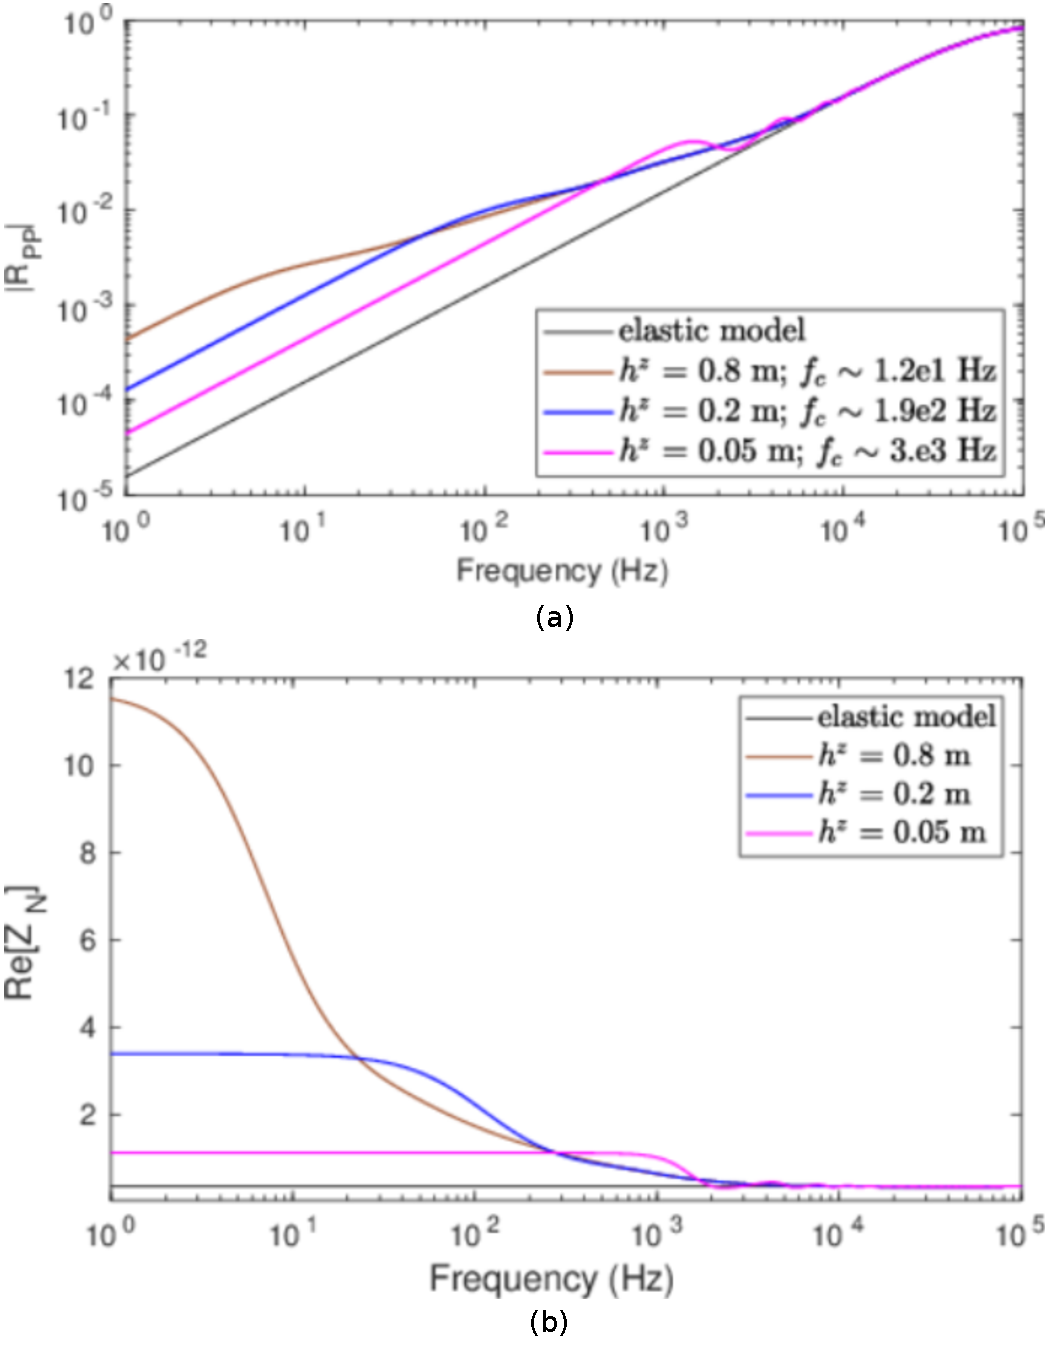
\includegraphics[width=90mm, height=110mm]{Figure4.pdf}
\caption {(a) Absolute value of normal-incidence P-wave reflection coefficient $|R_{PP}|$ and (b) real part of normal fracture compliance $Z_N$ as functions of frequency using a DZ permeability of 0.1 D and different DZ thicknesses $h^z$.}
\label{fig:4}
\end{figure}

\begin{figure}
\centering
        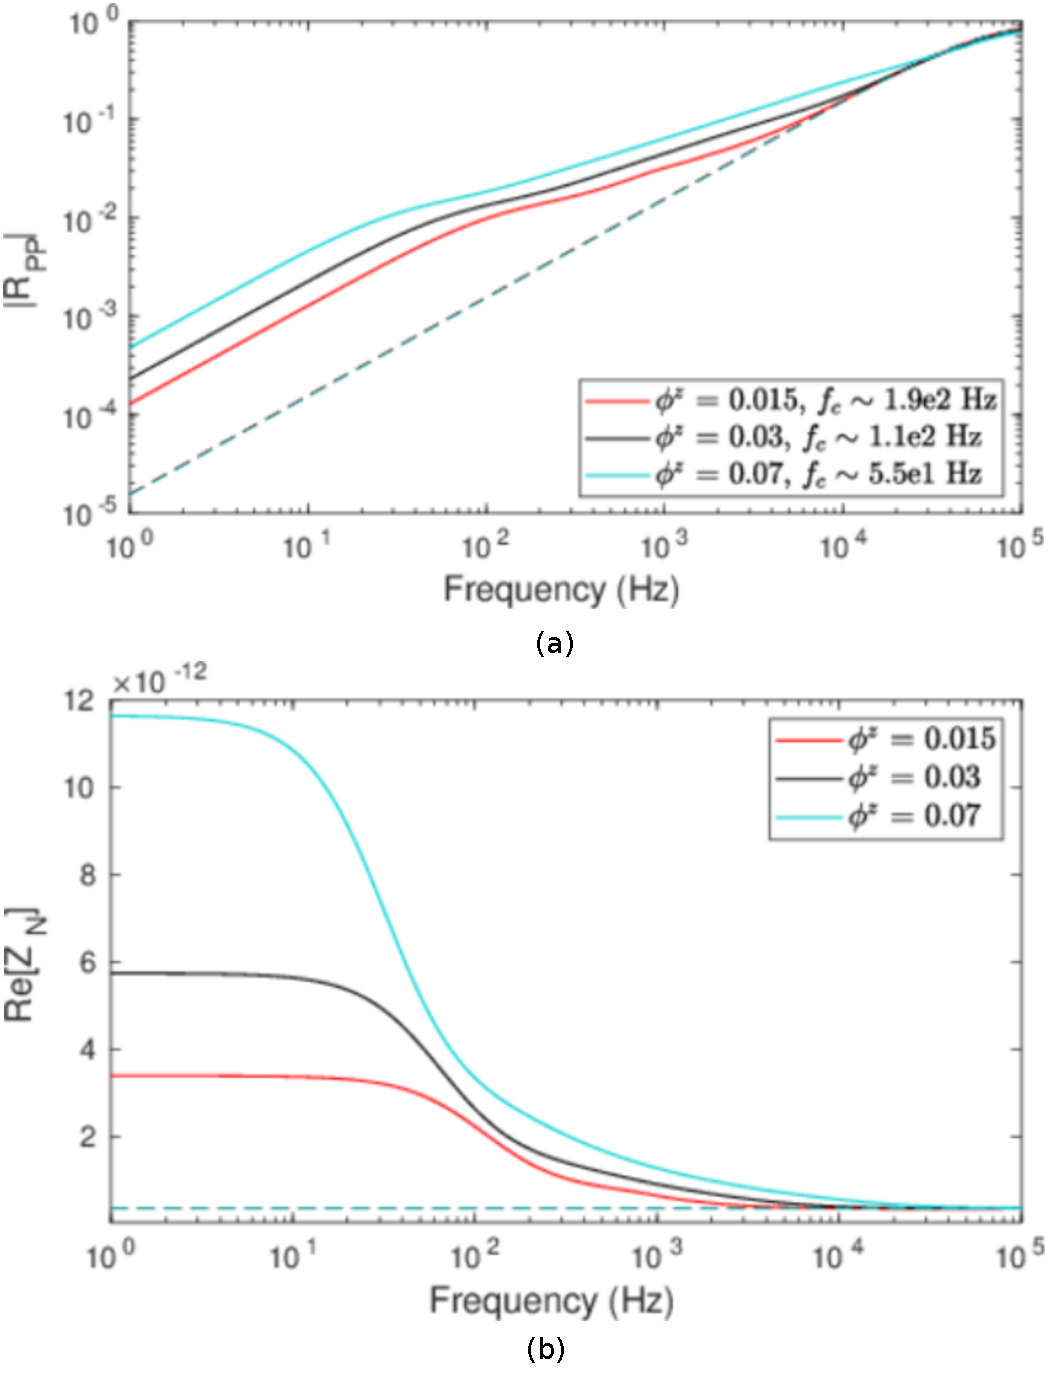
\includegraphics[width=90mm, height=110mm]{Figure5.pdf}
\caption { 
(a) Absolute value of normal-incidence P-wave reflection coefficient $|R_{PP}|$ and (b) real part of normal fracture compliance $Z_N$ as functions of frequency. Solid curves correspond to the elastic-poroelastic models generated using a DZ permeability of 0.1 D and various DZ porosities $\phi^z$. For these models, the background has the same rock physical properties as the DZ. Dashed lines denote the corresponding elastic models.
}
\label{fig:5}
\end{figure}

\subsection{Effect of DZ mechanical moduli}
In this section, we study the effect of decreasing the drained bulk and shear moduli  $K_m$ and $\mu$ of the DZ  on reflectivity and normal fracture compliance. The material properties for the reference elastic model and elastic-poroelastic model are taken from Table \ref{table:1}. For all models, the background has the same rock properties of the DZ.
For this example  (Figure \ref{fig:6}), we consider the decrease of the reference $K_m^z$ (Table \ref{table:1}) to 19.8 GPa and 6.6 GPa, corresponding to  60\%  and 20\% of its original value, respectively,  while keeping a fixed $K_m^z/\mu^z$ ratio of 1.14. This ratio corresponds to that of the reference mechanical moduli.
Solid lines in Figure \ref{fig:6}a show  $|R_{PP}|$ as a function of frequency for a DZ permeability $ \kappa^z $ of 0.1 D and varying values of DZ bulk modulus $K_m^z$. Dashed lines refer to the results of the corresponding elastic models.
Figure \ref{fig:6}b shows the real part of $Z_N$ for the same DZ parameters. Note that the reflectivity of the elastic models decreases with decreasing bulk modulus of the background and DZ (Figure \ref{fig:6}a). This is the result of the lower impedance  contrast between the background and the DZ-fracture system produced by the decreasing values of the background  and DZ mechanical moduli. On the other hand, the maximum increase of reflectivity due to FPD does not present such a  monotonic trend.
For a  $K_m^z$ of 19.8 GPa, there is not appreciable difference in the maximum increase of reflectivity when compared to the  reference case ($K_m^z$ = 33 GPa). On the contrary, for a  $K_m^z$ of 6.6 GPa, it is evident that the maximum increase of reflectivity is much lower than for the other two cases. Regarding the impact on normal fracture compliance, Figure \ref{fig:6}b shows that decreasing the mechanical moduli results in a higher maximum increase of normal fracture compliance, which is an opposed effect to that on the maximum increase of reflectivity (Figure \ref{fig:6}a). That is, that the decrease of the mechanical moduli, in general, decreases the maximum reflectivity of the DZ-fracture system.
These opposed results occur because the decrease of the mechanical  moduli has opposite effects on the induced FPD between the poroelastic fracture and associated DZ compared compared to its effect on the acoustic impedance contrast  between the background and the DZ-fracture poroelastic system. The aforementioned impedance contrast decreases with decreasing $K_m^z$, producing a decrease in the maximum reflectivity of the elastic-poroelastic system. In contrast,
Figure \ref{fig:6}b indicates that the decrease of mechanical moduli promotes FPD, which, in turn, has a positive impact on the maximum increase of normal fracture compliance. The latter can be explained by the opposed effects between the terms in the numerator and denominator involved in the calculation of the low-frequency limit of normal fracture compliance $Z_N^o$ (equation \eqref{Eq.23}). In the numerator, we have that as the DZ bulk modulus $K_m^z$ decreases, the DZ Skempton's coefficient $B^z$ increases, leading to lower values of $B^c-B^z$. This, in turn, decreases $Z_N^o$. However, in the denominator, we have that the term $M^z(1-\alpha^z B^z)$ decreases with lower values of $K_m^z$, which promotes a increase of $Z_N^o$.  For the values of $K_m^z$ used in this example, in combination with the particular rock and fluid properties of Table \ref{table:1}, we find that the denominator has a stronger influence on $Z_N^o$ and it leads to a increase of the the maximum fracture normal compliance with decreasing $K_m^z$. 

\begin{figure}
\centering
        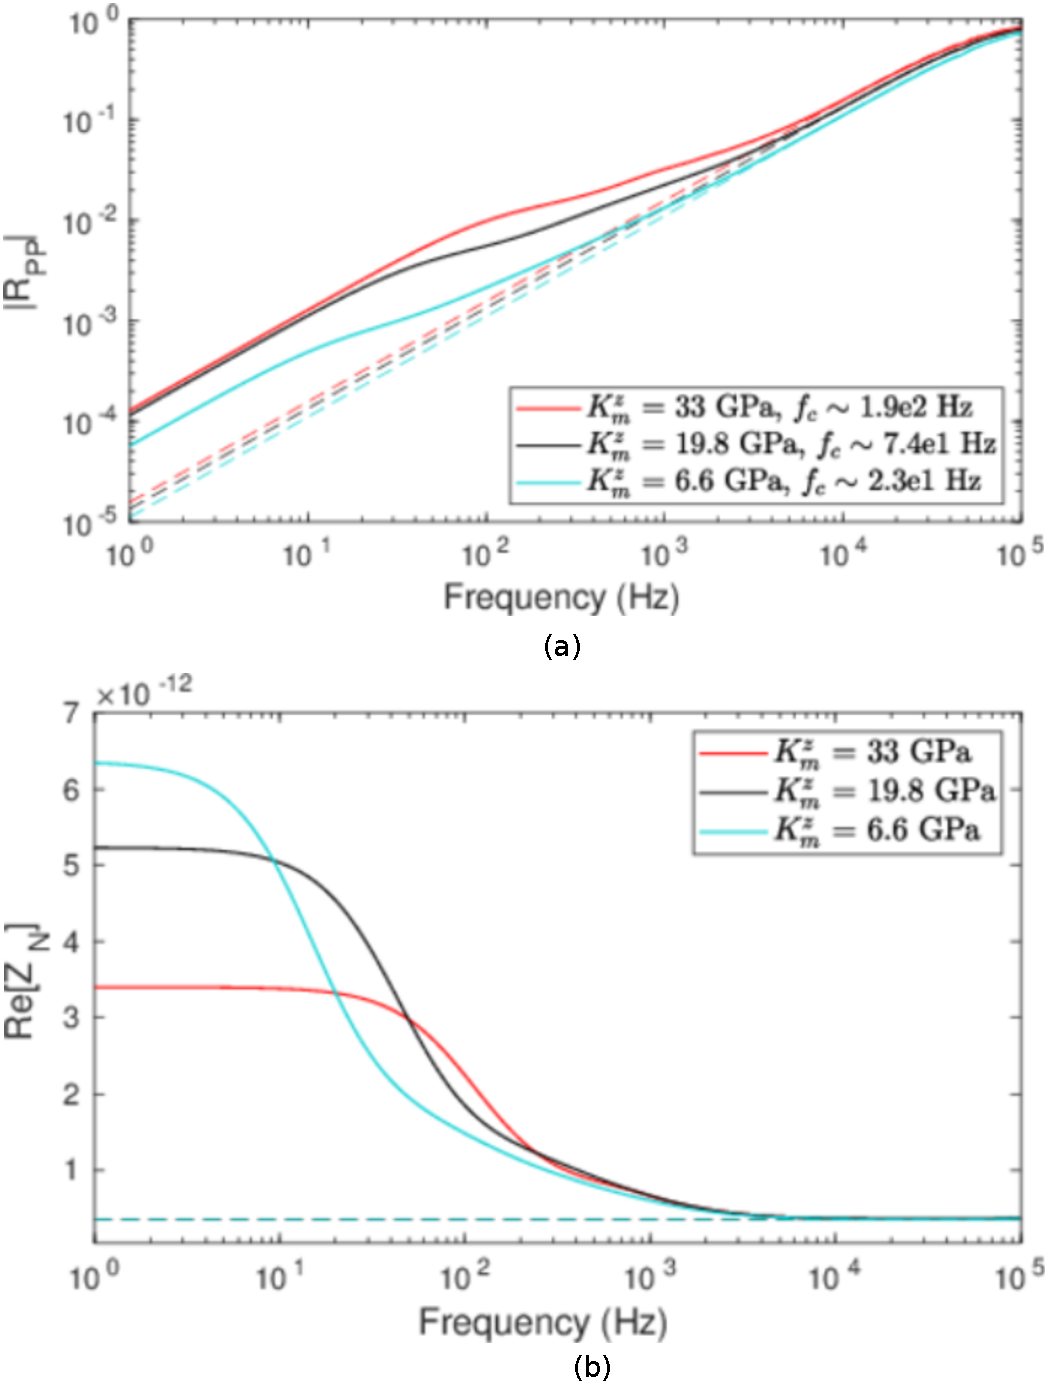
\includegraphics[width=80mm, height=110mm]{Figure6.pdf}
\caption {(a) Absolute value of normal-incidence P-wave reflection coefficient $|R_{PP}|$ and (b) real part of normal fracture compliance $Z_N$ as functions of frequency.  Solid curves correspond to elastic-poroelastic models
generated using a DZ permeability of 0.1 D and different DZ  $K_m^z$ moduli with $K_m^z/\mu^z$ = 1.14. For these models the background has the same rock properties as the DZ. Dashed lines denote the corresponding elastic models. }
\label{fig:6}
\end{figure}

\subsection{Effect of fracture mechanical  moduli}
Figures \ref{fig:7} and \ref{fig:8} show the effect of fracture thickness on reflectivity and normal compliance. However, this is equivalent to studying the effect of fracture moduli since both the thickness of the fracture and its mechanical moduli are related by equation (\ref{Eq.24}). Specifically, Figures \ref{fig:7} and \ref{fig:8} show the effect of two fracture thicknesses, \num{5e-3} m and \num{2e-4} m, respectively, on reflectivity and normal fracture compliance. To find the corresponding bulk and shear moduli, we use equation (\ref{Eq.24}), keeping  $Z_T^d$ and $Z_N^d$ constant and equal to 
\num{5e-10} m/Pa and \num{1.5e-10} m/Pa, respectively. For the fracture with a  thickness of \num{5e-3} m, the corresponding values for $K_m$ and $\mu$ are 0.02 GPa and 0.01 GPa. Similarly, for the fracture  with a thickness of \num{2e-4} m, the corresponding values for $K_m$ and $\mu$ are  \num{8e-4} GPa and  \num{4e-4} GPa. When comparing the corresponding reflectivities $|R_{PP}|$ in Figures \ref{fig:7}a and \ref{fig:8}a, we find that it is higher for the thicker fracture. However, the maximum increase of reflectivity due to FPD effects is higher for the thinner fracture. This increase for the thinner fracture is more than one order-of magnitude (Figure \ref{fig:8}a) compared to only a tenth of that increase for the thicker fracture (Figure \ref{fig:7}a). 
A similar trend is also evident from the corresponding  normal fracture compliance plots in Figures \ref{fig:7}b and \ref{fig:8}b, with a larger increase of maximum normal compliance for the thinner and softer fracture. In fact, we find that the  $Z_N^o/Z_N^u$ ratios are 2.67 and 43.35 for the thicker and thinner fractures, respectively. We also remark that the transition frequencies are the same as the ones shown in Figure \ref{fig:2} since we have not modified the properties of the DZ.

\begin{figure}
\centering
        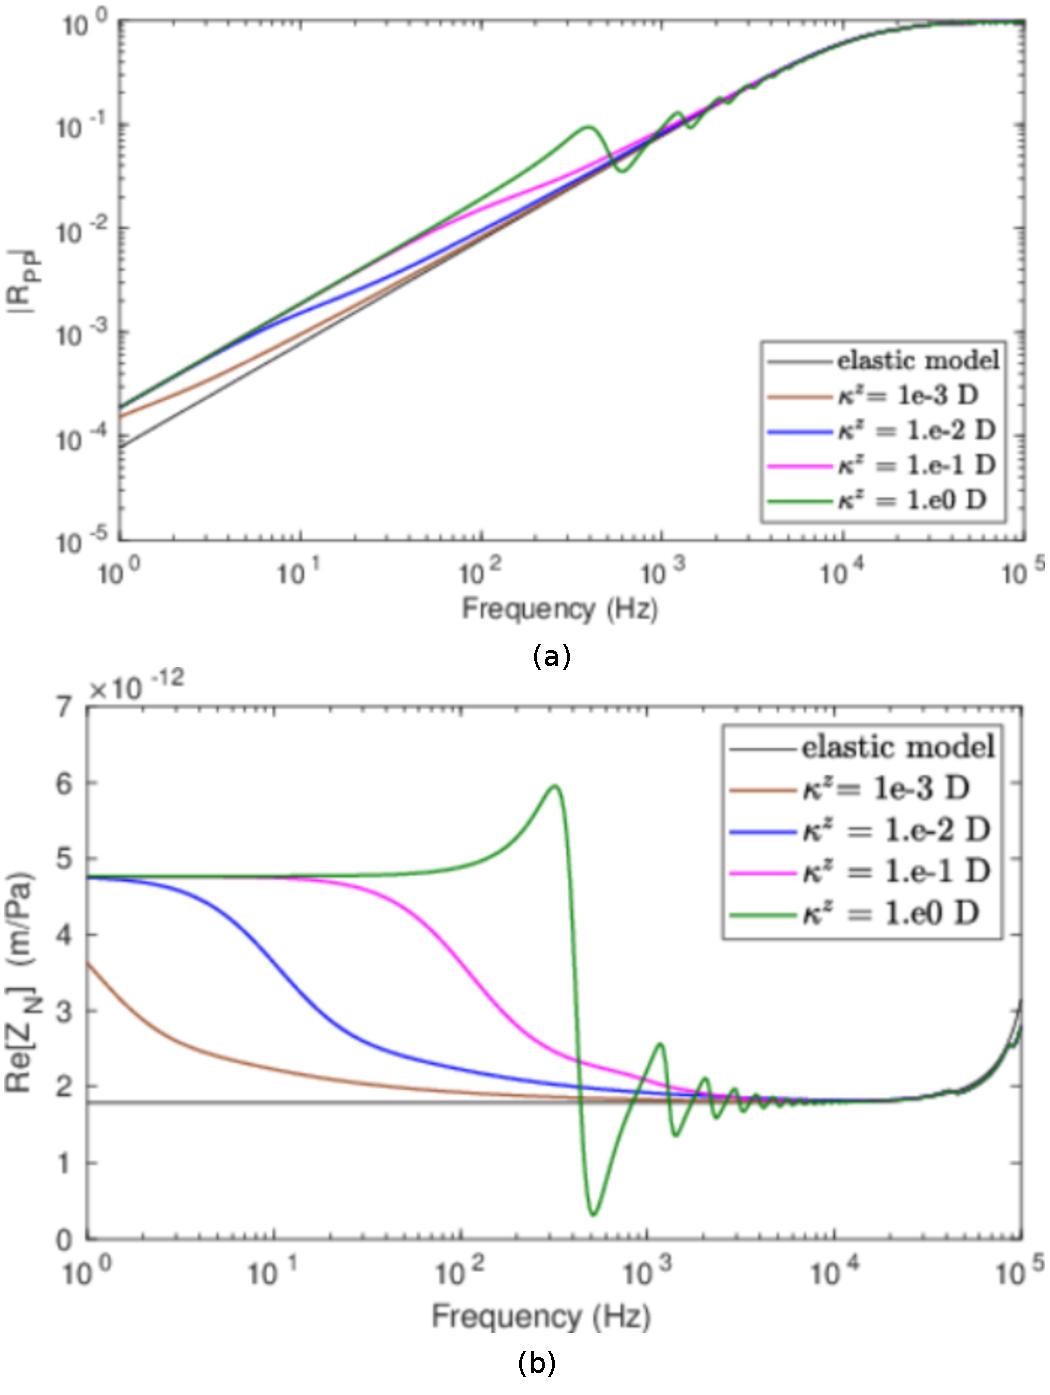
\includegraphics[width=80mm, height=110mm]{Figure7.pdf}
\caption {(a) Absolute value of normal-incidence P-wave reflection coefficient $|R_{PP}|$ and (b) real part of normal fracture compliance $Z_N$ as functions of frequency for different DZ permeabilities $\kappa^z$ for a fracture with a thickness of \num{5e-3} m.}
\label{fig:7}
\end{figure}

\begin{figure}
\centering
        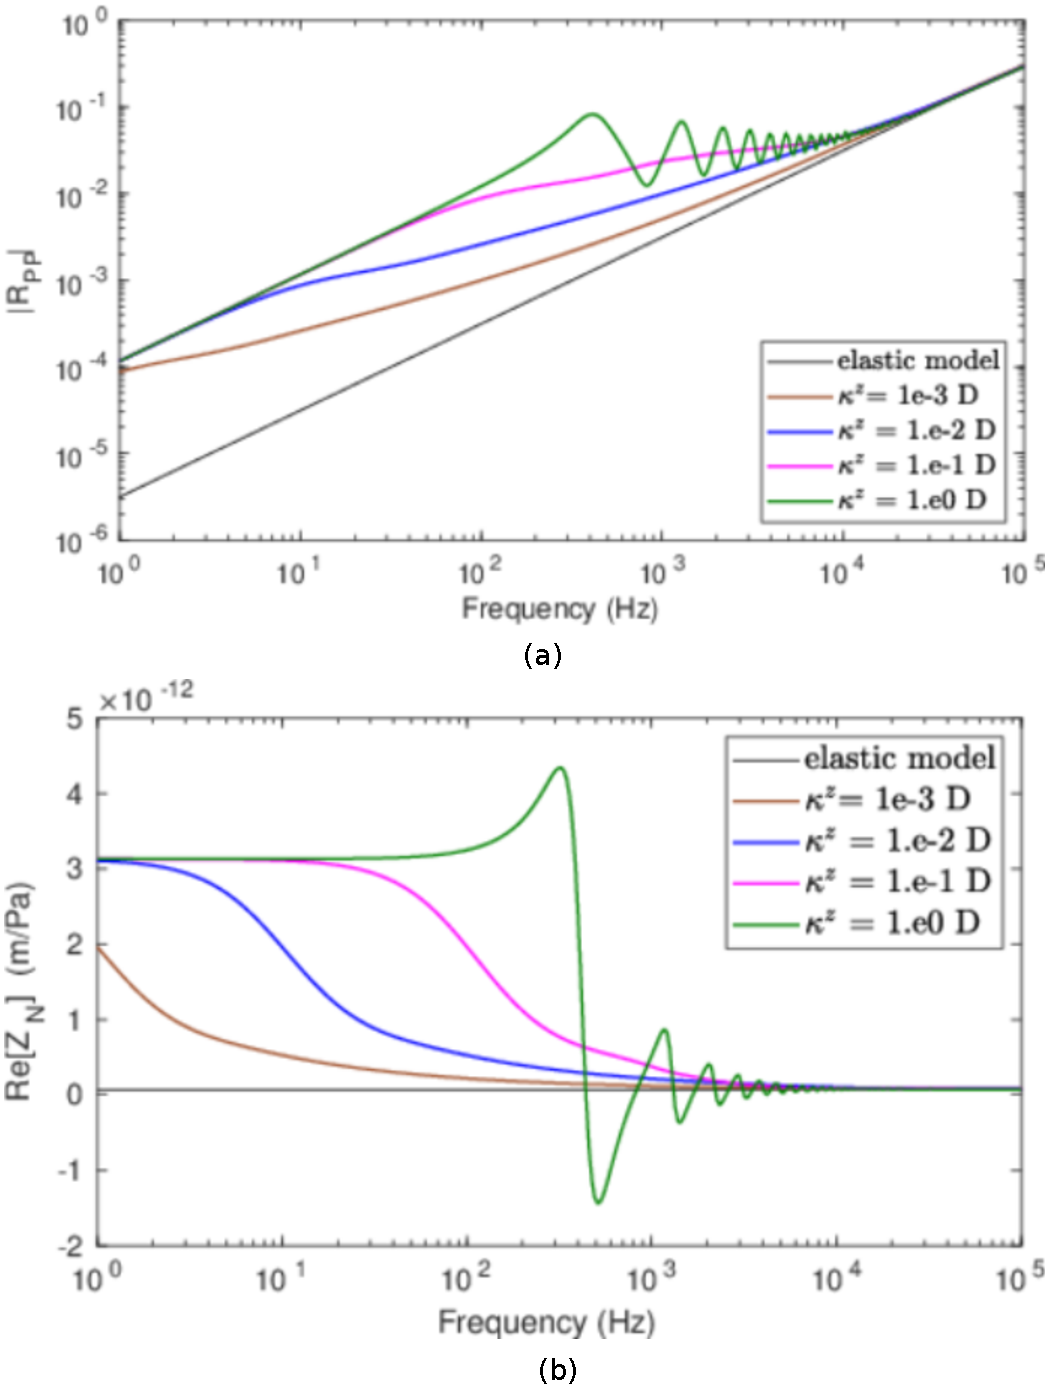
\includegraphics[width=73mm, height=90mm]{Figure8.pdf}
\caption {(a) Absolute value of normal-incidence P-wave reflection coefficient $|R_{PP}|$ and (b) real part of normal fracture compliance $Z_N$ as functions of frequency for different DZ permeabilities $\kappa^z$ for a fracture with a thickness of \num{2e-4} $m$.}
\label{fig:8}
\end{figure}

\subsection{Effect of a more compressible and less viscous pore fluid in the DZ and fracture}
Next, we study the effect of a more compressible and less viscous fluid, such as supercrital  CO$_2$ (Figure \ref{fig:9}), filling the pores of the fracture and the associated DZ in both elastic-poroelastic and purely elastic models. 
We set the supercritcal CO$_2$ properties $K_f$, $\rho_f$ and $\eta$ to 0.0229 GPa, 693 Kg/m$^3$ and \num{1.56e-5} Pa.s, respectively. These values are taken from \citeA{Rubino2011}. 
Figure \ref{fig:9}a shows that the elastic reflectivity obtained in such scenario is close to two orders-of-magnitude higher than the one obtained using water as the saturating fluid (Table \ref{table:1} and Figure \ref{fig:2}). However, the maximum increase of reflectivity due to FPD  is less than half of that obtained with water as saturating fluid (Figure \ref{fig:2}). 
A similar trend is observed for the normal fracture compliance, with  higher values for the elastic normal compliance when using supercritical CO$_2$ as the saturating fluid, of order of \num{1e-11} m/Pa, (Figure \ref{fig:9}b) than for the case of water as the saturating fluid,  order of \num{1e-12} m/Pa (Figure \ref{fig:3}a). Nonetheless, the maximum increase in compliance due to FPD effects is less for the case of CO$_2$ as saturating fluid, as indicated by its lower  $Z_N^o/Z_N^u$ ratio of 3.51 compared to the case of  water as  saturating fluid, with a higher $Z_N^o/Z_N^u$ ratio of 9.45.
Thus, even though the  fracture-DZ poroelastic system saturated with CO$_2$ is more seismically visible than its water-saturated counterpart, FPD effects are not as important.
This lower increase in normal fracture compliance and reflectivity happens because CO$_2$ has a much higher compressibility, of around two orders-of-magnitude, as compared to water.  This prevents a significant increase of fluid pressure inside the fracture from taking place, even though the fracture is being heavily deformed. Therefore, the fluid pressure gradient between the fracture and the DZ is smaller, and so are the FPD effects.
Another effect of considering supercritical CO$_2$ as the pore fluid is the decrease of the transition frequency $f_c$ for a given DZ permeability, which is around 10 \% with respect to the water-saturated case. This is the result of the higher impact of the reduction of  fluid compressibility compared to the impact of the decrease of its viscosity (equations \eqref{Eq.19} and \eqref{Eq.21}). We also observe the earlier onset of reverberations in Figure \ref{fig:9} than for the reference case (Figures \ref{fig:2} and \ref{fig:3}a ) for the curves corresponding to DZ permeabilities of 1 D and \num{1 e-1} D, respectively. This is consequence of much lower values of Biot's frequency for the DZ of $\sim$ \num{1.8e1} Hz and $\sim$ \num{1.8e2} Hz for the respective DZ permeabilites, caused by the lower fluid viscosity.

\begin{figure}[hp]
\centering
        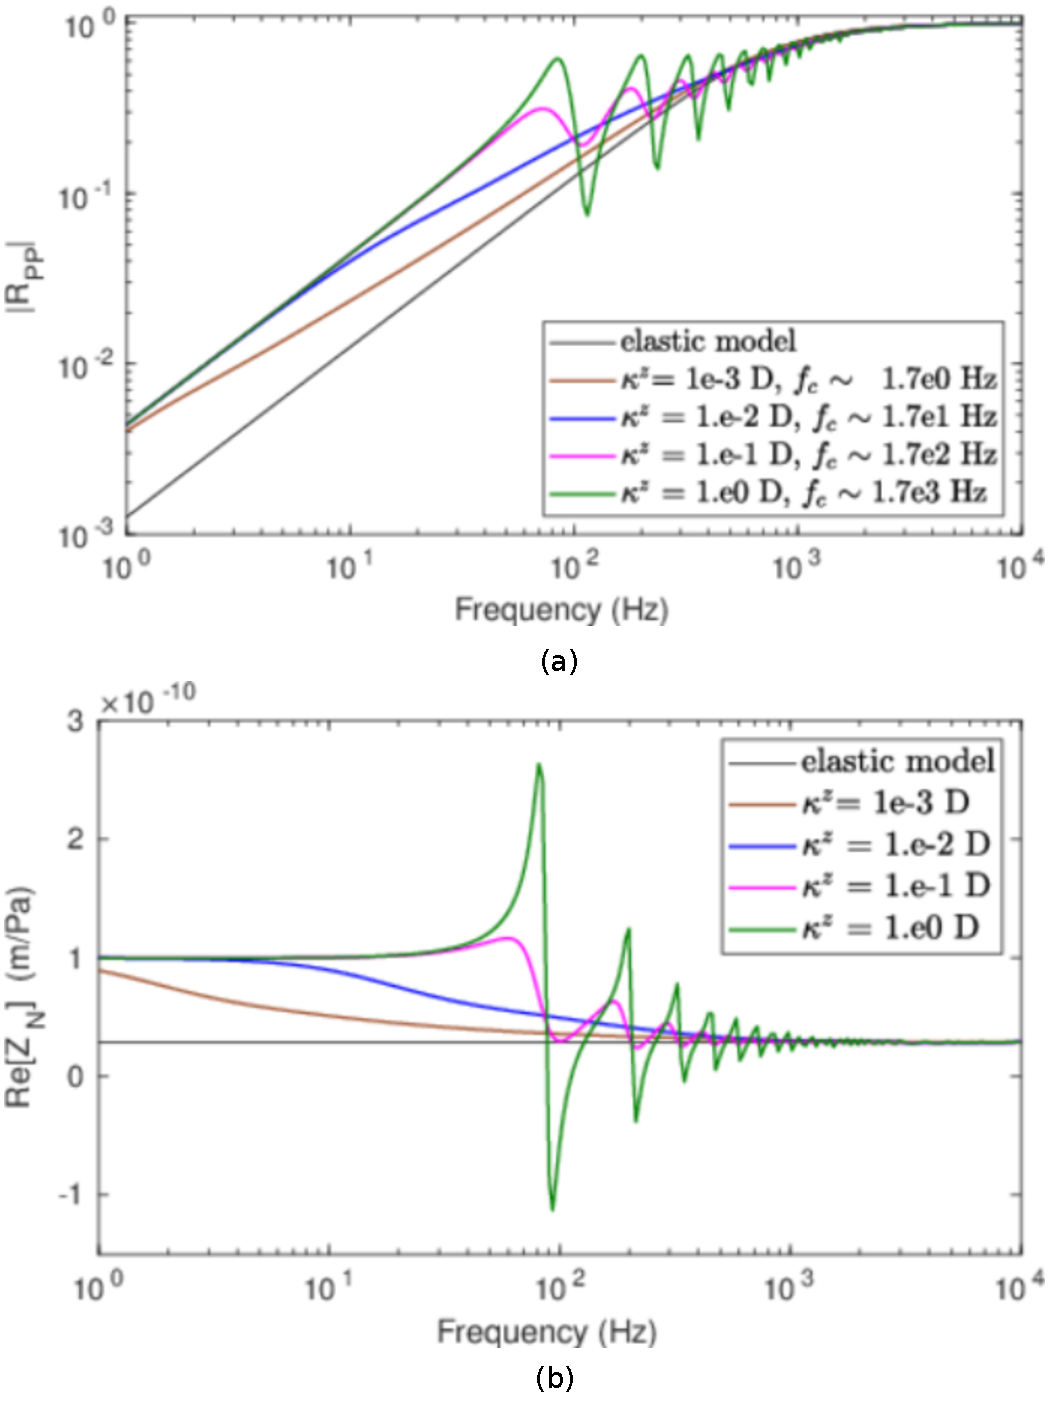
\includegraphics[width=85mm, height=110mm]{Figure9.pdf}
\caption {(a) Absolute value of normal-incidence P-wave reflection coefficient $|R_{PP}|$ and (b) real part of normal fracture compliance $Z_N$ as functions of frequency for different DZ permeabilities $\kappa^z$ considering supercritical CO$_2$ as the saturating pore fluid for the fracture and associated DZ.}
\label{fig:9}
\end{figure}

\subsection {Sensitivity analysis of the maximum increase of normal fracture compliance}

We have shown in the previous examples the effect of discrete variations of rock and fluid properties of the DZ and fracture on the maximum increase of normal fracture compliance due to FPD. In this section, we investigate in more detail the sensitivity of the maximum increase of normal fracture compliance to the  changes of rock and fluid properties. These properties are changed one at a time while keeping the other ones constant and equal to the values shown in Table \ref{table:1}.

We let the $Z_N^o/Z_N^u$ ratio be a measure of the maximum increase of normal fracture compliance due to FPD. According to equation (\ref{Eq.23}), $Z_N^o$ is the low-frequency limit of normal compliance of the fracture. This means that it is the maximum value that it can take because at this frequency limit FPD is on its relaxed regime,  causing the largest possible volume of fluid  to exit the fracture. This, in turn, decreases to a minimum the fluid stiffening effect in the fracture. In contrast, $Z_N^u$ is the high-frequency limit of the normal compliance of the fracture, indicating that this is the lowest value that it can take because, at this frequency limit, the unrelaxed FPD regime prevails, which implies that the fracture behaves as hydraulically isolated. At this stage, the normal compliance value is that of an elastic fracture. Therefore, the  $Z_N^o/Z_N^u$ ratio provides a measure of the maximum increase of normal fracture compliance due to FPD  with respect to its elastic limit. To show how this maximum increase is controlled by the rock and fluid properties, we plot the $Z_N^o/Z_N^u$ ratio as a function of dimensionless properties $X$ (Figure \ref{fig:10}), where $X$ indicates the factor by which a reference property value has increased. Table \ref{table:2} lists the different dimensionless properties that $X$ represent as well as the corresponding reference value.
We remark that the response of $Z_N^o/Z_N^u$ to the variations $\bar{K}_m^c$ and $\bar{K}_m^z$ also includes the effect of the respective shear moduli changes. Nonetheless, we only show the values that the dimensionless bulk moduli take.
For the case of the fracture, we find  both the bulk and shear modulus by means of equation (\ref{Eq.24}). To this end, we vary the thickness of the fracture from \num{e-4} m to \num{e-2} m, while keeping constant the tangential and drained normal compliance to \num{5e-10} m/Pa and \num{1.5e-10} m/Pa, respectively. Then, the reference modulus $\tilde{K}_m^c$ corresponds to that found with a fracture thickness of \num{e-4} m. For the case of the DZ, we simply assume that the bulk modulus is 1.14 times the value of the shear modulus. This ratio is the same as the one corresponding to the DZ moduli in Table \ref{table:1}.

Figure \ref{fig:10} shows that the increase of most of the dimensionless rock and fluid properties produces either a monotonic increase or decrease of the $Z_N^o/Z_N^u$ ratio. Properties producing an increase of $Z_N^o/Z_N^u$ as they increment are $\bar{\phi}^z$, $\bar{h}^z$ and $\bar{K_f}$. As already investigated in the previous examples, the increase of $\bar{\phi}^z$ and $\bar{h}^z$ has a positive impact on the maximum increase of normal fracture compliance because they provide a greater pore volume for FPD. On the other hand, an increasingly stiffer fluid $\bar{K_f}$, creates the necessary pressure gradient for FPD.
In contrast, the increment of $\bar{K}_m^c$ produces a continuous decrease of the $Z_N^o/Z_N^u$ ratio because the fracture becomes increasingly stiffer. However,  $\bar{K}_m^z$  is the only property, among the ones studied, that does not produce a monotonic response of the  $Z_N^o/Z_N^u$ ratio. We observe that, for sufficiently low values of $\bar{K}_m^z$, the increase of this property causes a continuous rise of  $Z_N^o/Z_N^u$ until a maximum  is reached. Then, a further increase of $\bar{K}_m^z$ produces a continuous decline of the $Z_N^o/Z_N^u$ ratio. 
The non-monotonic behavior of  $Z_N^o/Z_N^u$ occurs as a consequence of the opposing effects that $B^z$ and $M^Z$ have on the DZ fluid pressure $p_f^z=- B^z \, H^z \, \nabla . \, \bm{u}^s - M ^z\, \nabla . \, \bm{w}$. That is, increasing values of $\bar{K}_m^z$ decreases $B^z$ and $B^z \, H^z$, and this, in turn, induces lower magnitudes of $p_f^z$,  which  will tend to promote higher pressure gradients for FPD, and as a consequence,  higher values of $Z_N^o$. On the contrary, increasing values of $\bar{K}_m^z$ increases $M^z$. This, in turn, induces higher magnitudes of $p_f^z$, which will tend to promote lower pressure gradients for FPD and, as a consequence, a reduction of $Z_N^o$.  
In section 3.3, we have  analyzed the effects of DZ moduli on the maximum increase of fracture normal compliance.
In that analysis we have found that for values of  $K_m^z \geq$ 6.6 GPa ($\bar{K}_m^z \geq$ 33), the maximum increase of normal fracture compliance decreases with the increase of  $K_m^z$. This  means that for the $K_m^z$  values used in that section, the response of the $Z_N^o/Z_N^u$  ratio is in the decreasing part of the curve.
Notice that, for this sensitivity analysis, we do not consider neither the permeability of the DZ nor the viscosity of the saturating fluid, because, according to equation \eqref{Eq.23}), none of these properties has any effect on the maximum increase on normal compliance. Nonetheless, these parameters control the transition frequency between FPD regimes (equations \eqref{Eq.19} and \eqref{Eq.21}).

For completeness, Table \ref{table:3} shows the $Z_N^o/Z_N^u$  ratios for the rock and fluid properties analyzed in the previous sections. Here, the column \emph{Marker} refers to the marker used in Figure \ref{fig:10} to plot the respective data entry.
These results can be compared against the  $Z_N^o/Z_N^u$ ratio  of 9.45 obtained for the reference elastic-poroelastic model using the properties of Table \ref{table:1}. The dimensionless variables of interest for the rock and fluid properties of Table \ref{table:1} are $\bar{h}^z$ = 20, $\bar{K}_m^z$ = 165, $\bar{K}_m^c$ = 10 and $\bar{K}_f^z$ = 225.

\begin{figure}
\centering
      {
        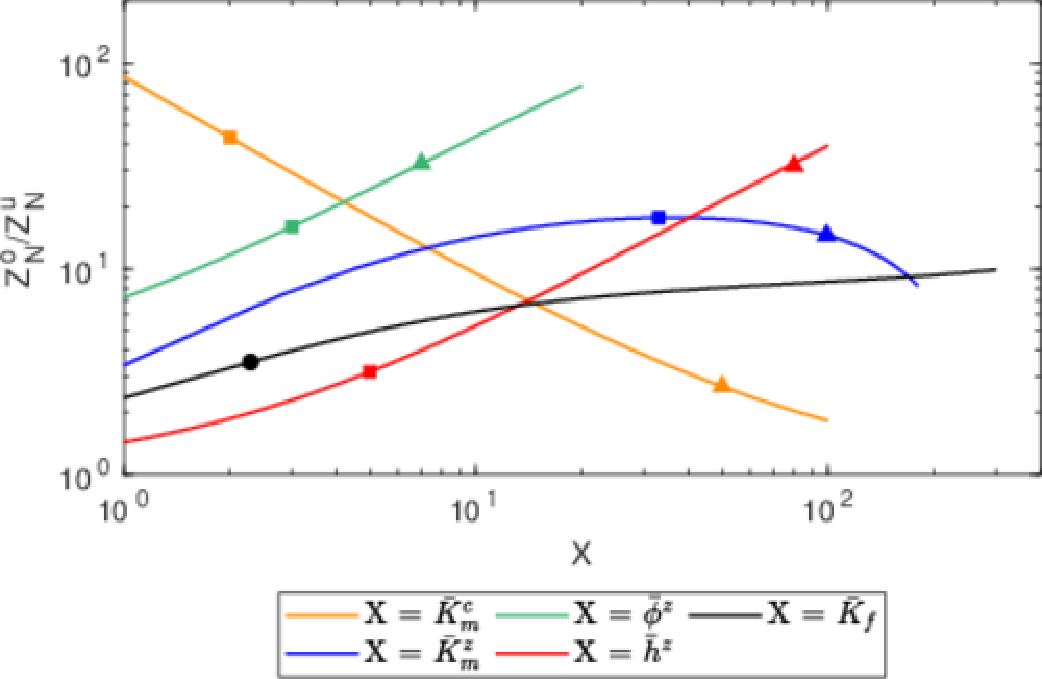
\includegraphics[width=85mm, height=55mm]{Figure10.pdf}
        }
\caption { $Z_N^o / Z_N^u$ ratio as a function of dimensionless rock and fluid properties $X$ obtained with normalization with corresponding reference values. Property $X$ represents the factor by which a reference value has increased. The corresponding dimensionless properties are: the increment of the fracture bulk modulus $\bar{K}_m^c$, the increment of the DZ bulk modulus $\bar{K}_m^z$, the increment of DZ thickness $\bar{h}^z$ and the increment of the fluid bulk modulus $\bar{K}_f$. The corresponding reference values are:  $\tilde{K}_m^c$ = \num{4e-4} GPa,  $\tilde{k}_m^z$ = 0.2 GPa, the thickness of DZ $ h^z$ = 0.01 m and $ K_f$ = 0.01 GPa. Markers denote data points as detailed in Table \ref{table:3}.
}
\label{fig:10}
\end{figure}

\begin{table}[!ht]
  \caption{Definition of the dimensionless properties and the corresponding reference values used for Figure \ref{fig:10}.}
\begin{center}
  \begin{tabular}{ | l | l| }
    \hline
    Dimensionless property $X$ & Reference value  \\ \hline
    Increment of fracture bulk modulus $\bar {K}_m^c$  & $\tilde{K}_m^c$ = \num{4e-4} GPa \\ 
    Increment of DZ bulk modulus $\bar {K}_m^z$  & $\tilde{K}_m^z$ = 0.2 GPa  \\
    Increment of DZ porosity $\bar{\phi}^z$  & $\tilde{\phi}^z$ = 0.01 \\
    Increment of DZ thickness $\bar{h}^z$ & $\tilde{h}^z$ = 0.01 m \\ 
    Increment of fluid bulk modulus $\bar{K}_f$ & $\tilde{K}_f$ = 0.01 GPa \\
    \hline
  \end{tabular}
  \label{table:2}
\end{center}
\end{table}

\begin{table}[!ht]
  \caption{$Z_N^o/Z_N^u$ ratio for the different rock and fluid properties studied in the previous examples. See Table \ref{table:2} for a description of the dimensionless properties and Figure \ref{fig:10} for the plots of the data points.}
\begin{center}
  \begin{tabular}{ | l | c | c| c| }
    \hline
    Property (dimensionless) & Property value (dimensionless) & $Z_N^o/Z_N^u$ & Marker \\
    \hline
    \multirow{2}{10em}{$h^z$  $\left( \bar{h}^z \right)$} & 0.05 m (5) & 3.15 & \color{red}\FilledSquare \\ 
     & 0.8 m (80) & 31.51 & \color{red}\FilledTriangleUp \\ 
    \hline
    \multirow{2}{10em}{$\phi^z$  $ \left(\bar{\phi}^z  \right)$} & 0.03  (3) & 15.96 & \color{green}\FilledSquare\\ 
     & 0.07  (7) & 32.35  & \color{green}\FilledTriangleUp \\ 
     \hline
        \multirow{2}{10em}{$K_m^z$ $ \left( \bar{K}_m^z \right)$} & 6.6 GPa (33) & 17.67 & \color{blue}\FilledSquare \\ 
     & 19.8 GPa (99) & 14.53  & \color{blue}\FilledTriangleUp \\ 
    \hline
     \multirow{2}{10em}{$K_m^c$ $ \left( \bar{K}_m^c \right)$} & \num{8e-4} GPa (2) & 43.35 & \color{orange}\FilledSquare \\ 
     & 0.02 GPa (50) & 2.67 & \color{orange}\FilledTriangleUp \\ 
    \hline
    $K_f$ $\left( \bar{K}_f \right)$  & 0.0229 GPa (2.29) & 3.51 & \color{black}\FilledCircle\\ 
    \hline
  \end{tabular}
  \label{table:3}
\end{center}
\end{table}


\section{Discussion}
In this work, we have shown that the presence of a DZ in low-permeability formations has the potential to increase the compliance and reflectivity of a fracture due to FPD in the seismic exploration frequency range. Specifically, our study indicates that the rock and fluid  physical properties of the DZ and fracture  have a direct control on the fluid exchange between these two regions due to FPD and, therefore, they determine the maximum increase of normal fracture compliance from its elastic limit.
However, the variation of rock properties may not produce the same trend on reflectivity as they do on the normal fracture compliance because these property changes may cause opposing results on FPD between the fracture and DZ and on the impedence contrast between the background and the poroelastic fracture-DZ system.
This response is observed, for instance, when decreasing the DZ and background mechanical moduli (Figure \ref{fig:8}). 
For the elastic-poroelastic models tested in that example, the maximum fracture normal compliance decreases but the maximum reflectivity in general increases with increasing values of $K_m^z$. In fact, it is possible to show that the maximum acoustic impedance contrast between the  background and the poroelastic fracture-DZ system increases with $K_m^z$. To this end,  the low-frequency limit P-wave velocity of the  poroelastic DZ-fracture system can be calculated as suggested by \citeA{Brajanovski2005}. We remind the reader that for these examples the mechanical moduli of the background is the same as those for the DZ. A corollary of these observations is that a 1D model considering a slip interface characterized by a poroelastic normal compliance, as the ones calculated in the examples presented in this work, does not, in principle, 
represent the seismic response of the poroelastic fracture-DZ system, since the acoustic impedance of this entire system is not accounted for. Nonetheless, we expect to explore models that are seismically equivalent to the aforementioned poroelastic system in future works.

We  have considered that the DZ and the adjacent impermeable background have the same rock properties except for the permeability, since we  have aimed to highlight the effects of FPD on reflectivity.
Thus, we have not analyzed the effect on reflectivity of any  decrease in mechanical moduli or increase in porosity in the DZ with respect to the background, although these effects are expected due to the presence of micro- and macro-fractures in the DZ. In Figure \ref{fig:11}, we present such an analysis. Here, solid lines correspond to elastic-poroelastic models for a DZ permeability of 0.1 D and dashed curves of the same color denote the corresponding elastic model. Unless stated otherwise, all other DZ properties are the same as in Table \ref{table:1}.
Figure \ref{fig:11}a shows the effect of the decrease of DZ bulk and shear moduli while the corresponding background moduli are kept constant. The red solid curve corresponds to the elastic-poroelastic model, for which the background and DZ have the same rock and fluid properties. The red dashed curve shows the reflectivity for the corresponding elastic model.
We observe that, compared to this elastic model, the other two present higher reflectivities.
The reason for this increase in reflectivity is the presence of a softer region comprised by the DZ and fracture that produces a higher impedance contrast with regard to the background: the elastic reflectivity increases as the DZ becomes softer. In contrast,  the maximum increase of reflectivity due to FPD from its corresponding elastic reference decreases as the DZ becomes softer. This is the consequence of the decreasing mechanical contrast between the DZ and the fracture. Nonetheless, it is likely that the DZ becomes not only softer but also more porous. Figure \ref{fig:11}b presents reflectivities of models considering  increasing porosities of a DZ that is softer than the background. As expected, the increase of the pore volume promotes FPD, increasing the maximum reflectivity from its elastic reference, thus counteracting the effect of the decrease of DZ bulk and shear moduli.
We assume that changes in porosity do not have any further effect on the bulk modulus of the DZ, although it is expected that an increase in porosity would decrease the bulk modulus. On the one hand, this would result in a higher impedance contrast with the stiffer background rock, on the other hand, however,  the softening of the DZ bulk modulus would decrease the FPD effects between the fracture and DZ (Figure  \ref{fig:10}).

\begin{figure}[hp]
\centering
        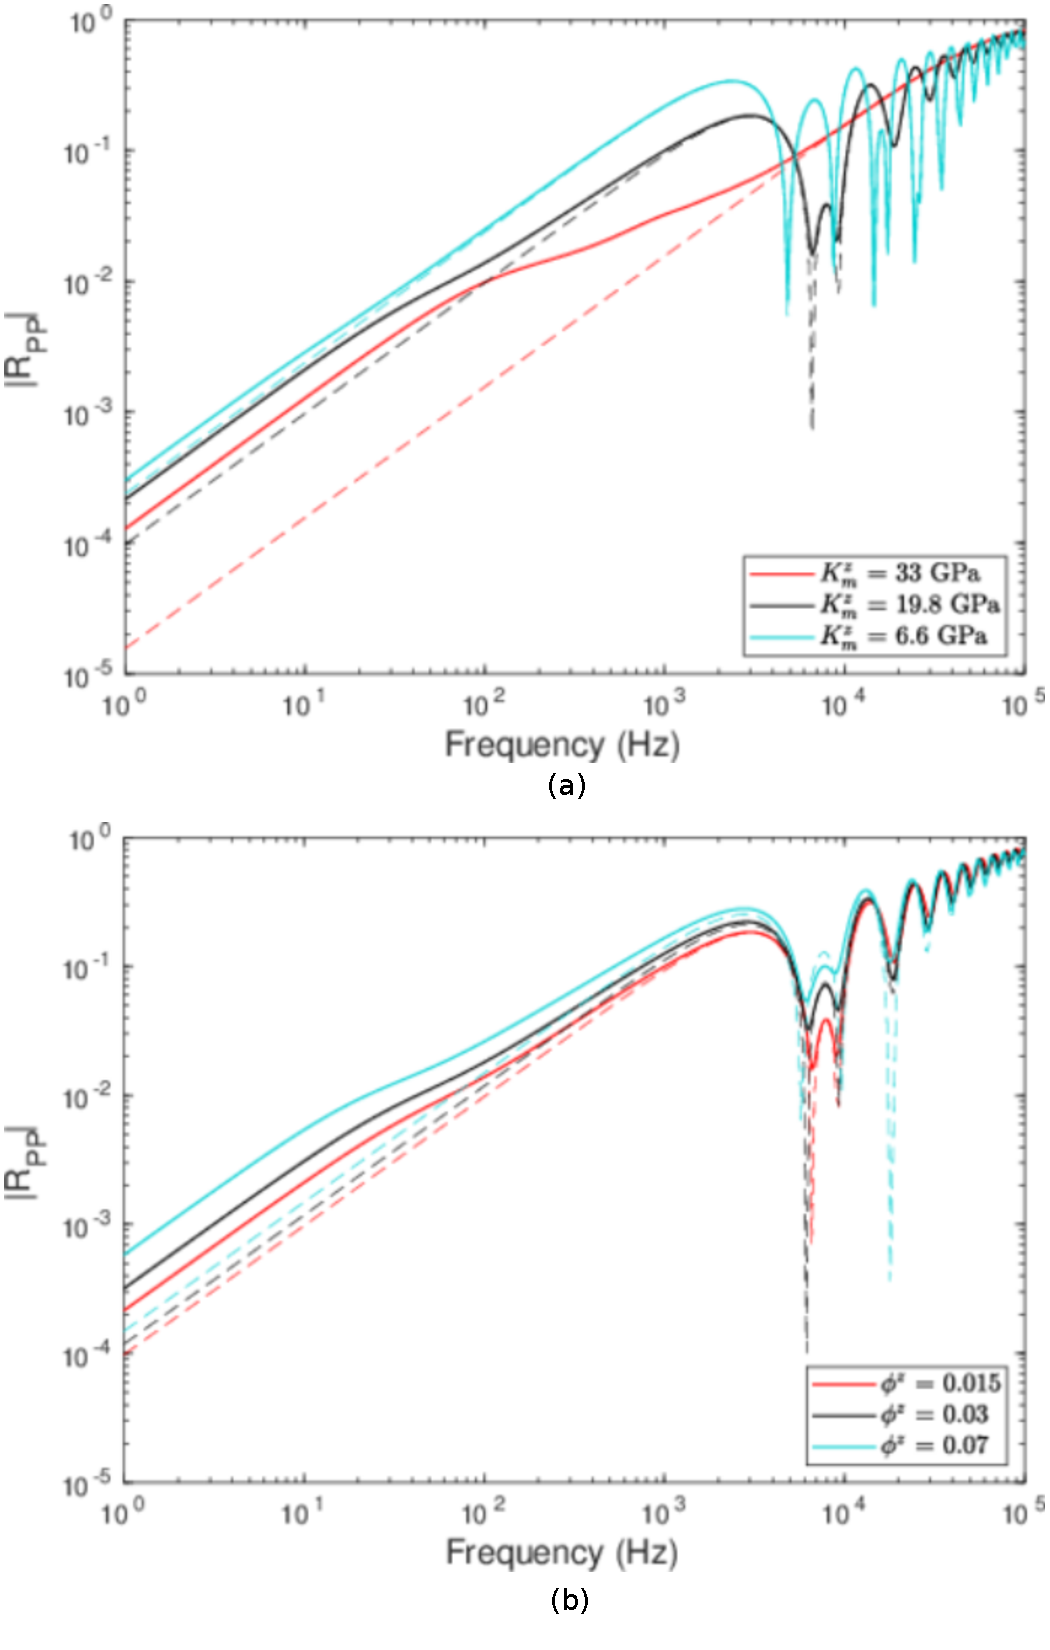
\includegraphics[width=80mm, height=120mm]{Figure11.pdf}
\caption {
Absolute value of normal-incidence P-wave reflection coefficient $|R_{PP}|$ as a function of frequency.
Solid lines correspond to elastic-poroelastic models for a DZ permeability of 0.1 D. Dashed lines of the same color denote the corresponding elastic models. (a) Curves for varying values of DZ bulk moduli $k_m^z$ with $k_m^z/\mu^z$  = 1.14. The background bulk modulus is kept constant to 33 GPa.
 (b) Curves for varying values of DZ porosity $\phi^z$. DZ bulk modulus $k_m^z$ is 19.8 GPa. }
\label{fig:11}
\end{figure}


We have shown that the FPD effects between an isolated fracture and its surroundings (DZ) even in largely impermeable rocks are evidenced by the fact that the normal fracture compliance becomes complex-valued, presenting the largest magnitude of its imaginary part when the energy dissipation is the greatest. This result provides a possible explanation for the existence of an imaginary part in seismic measurements 
even if the background is largely impermeable  \cite{Barbosa2019}. Furthermore, our results regarding the enhanced reflectivity in the seismic frequency band further imply that FPD between the fracture and its associated DZ could be an important factor, for which reflectivity from fractures can be distinguished using seismic exploration techniques even in largely impermeable environments \cite<e.g.,>{Kim1994, Schmelzbach2007}.

Future research should consider more realistic configurations of the DZ. For instance, these models should include the effect of discrete fractures in the DZ. However, to be able to calculate the reflectivity  with a semi-analytical approach of a poroelastic system comprised by an isolated fractured and such a complex DZ representation, it would be necessary to upscale this system using techniques such as the one proposed by \citeA{Rubino2016}. The isolated fracture and associated complex DZ could then be represented by an equivalent anisotropic viscoelastic medium. Another approach would be to consider the fracture-complex DZ poroelastic system as an equivalent viscoelastic slip interface. Meaning that the entire poroelastic system is modeled as a displacement-jump interface characterized by complex-valued, frequency-dependent compliances.
However, this representation would be valid only for poroelastic fracture-DZ systems with thicknesses much smaller than the prevailing seismic wavelengths.


\section{Conclusions}
We have considered a layered model to analyze the poroelastic effects associated with a DZ adjacent to a fracture  in a low-permeability background rock.
Our results show that FPD between a fracture and its adjacent DZ increases fracture normal compliance, as this process allows fluid pressure release from the fracture into the DZ.
As a consequence, the reflectivity of the system also increases compared to an impermeable reference model. 
Our results also show that the maximum  increase of normal compliance  and reflectivity are most sensitve to the increase in DZ thickness and porosity as well as to to the decrease of fracture mechanical moduli. In contrast, the permeability of the DZ does not have any effect in the maximum increase of reflectivity but controls the transition frequency between FPD regimes and, therefore, constrains the visibility of the FPD effects on reflectivity: the greater the permeability of the DZ, the higher the transition frequency to the unreleaxed FPD regime, which allows  for a wider range of frequencies for FPD to contribute in its relaxed regime. The thickness and porosity of the DZ affect both the maximum increase of reflectivity and the transition frequency. Greater thicknesses and porosities increase the reflectivity of the system but shift the transition frequency to lower values. The consequence of this latter is that the visibility of FPD effects on  reflectivity is constrained to lower frequency bands. In this regard, an increase of the DZ thickness and porosity has an opposing effect to that of an increase of the DZ permeability.
Regarding the effect of decreasing the mechanical moduli of the DZ, our results show that this decrease limits to lower values the maximum increase of reflectivity due to FPD. However, this effect is opposed by a likely increase of DZ porosity.
Overall, this study shows that FPD effects promoted by the presence of a DZ in an otherwise largely impermeable background can  notably enhance the reflectivity of a fracture in the seismic frequency band.



%Text here ===>>>
%%

%  Numbered lines in equations:
%  To add line numbers to lines in equations,
%  \begin{linenomath*}
%  \begin{equation}
%  \end{equation}
%  \end{linenomath*}



%% Enter Figures and Tables near as possible to where they are first mentioned:
%
% DO NOT USE \psfrag or \subfigure commands.
%
% Figure captions go below the figure.
% Table titles go above tables;  other caption information
%  should be placed in last line of the table, using
% \multicolumn2l{$^a$ This is a table note.}
%
%----------------
% EXAMPLE FIGURES
%
% \begin{figure}
% \includegraphics{example.png}
% \caption{caption}
% \end{figure}
%
% Giving latex a width will help it to scale the figure properly. A simple trick is to use \textwidth. Try this if large figures run off the side of the page.
% \begin{figure}
% \noindent\includegraphics[width=\textwidth]{anothersample.png}
%\caption{caption}
%\label{pngfiguresample}
%\end{figure}
%
%
% If you get an error about an unknown bounding box, try specifying the width and height of the figure with the natwidth and natheight options. This is common when trying to add a PDF figure without pdflatex.
% \begin{figure}
% \noindent\includegraphics[natwidth=800px,natheight=600px]{samplefigure.pdf}
%\caption{caption}
%\label{pdffiguresample}
%\end{figure}
%
%
% PDFLatex does not seem to be able to process EPS figures. You may want to try the epstopdf package.
%

%
% ---------------
% EXAMPLE TABLE
%
% \begin{table}
% \caption{Time of the Transition Between Phase 1 and Phase 2$^{a}$}
% \centering
% \begin{tabular}{l c}
% \hline
%  Run  & Time (min)  \\
% \hline
%   $l1$  & 260   \\
%   $l2$  & 300   \\
%   $l3$  & 340   \\
%   $h1$  & 270   \\
%   $h2$  & 250   \\
%   $h3$  & 380   \\
%   $r1$  & 370   \\
%   $r2$  & 390   \\
% \hline
% \multicolumn{2}{l}{$^{a}$Footnote text here.}
% \end{tabular}
% \end{table}

%% SIDEWAYS FIGURE and TABLE
% AGU prefers the use of {sidewaystable} over {landscapetable} as it causes fewer problems.
%
% \begin{sidewaysfigure}
% \includegraphics[width=20pc]{figsamp}
% \caption{caption here}
% \label{newfig}
% \end{sidewaysfigure}
%
%  \begin{sidewaystable}
%  \caption{Caption here}
% \label{tab:signif_gap_clos}
%  \begin{tabular}{ccc}
% one&two&three\\
% four&five&six
%  \end{tabular}
%  \end{sidewaystable}

%% If using numbered lines, please surround equations with \begin{linenomath*}...\end{linenomath*}
%\begin{linenomath*}
%\begin{equation}
%y|{f} \sim g(m, \sigma),
%\end{equation}
%\end{linenomath*}

%%% End of body of article

%%%%%%%%%%%%%%%%%%%%%%%%%%%%%%%%
%% Optional Appendix goes here
%
% The \appendix command resets counters and redefines section heads
%
% After typing \appendix
%
%\section{Here Is Appendix Title}
% will show
% A: Here Is Appendix Title
%
%\appendix
%\section{Here is a sample appendix}

%%%%%%%%%%%%%%%%%%%%%%%%%%%%%%%%%%%%%%%%%%%%%%%%%%%%%%%%%%%%%%%%
%
% Optional Glossary, Notation or Acronym section goes here:
%
%%%%%%%%%%%%%%
% Glossary is only allowed in Reviews of Geophysics
%  \begin{glossary}
%  \term{Term}
%   Term Definition here
%  \term{Term}
%   Term Definition here
%  \term{Term}
%   Term Definition here
%  \end{glossary}

%
%%%%%%%%%%%%%%
% Acronyms
%   \begin{acronyms}
%   \acro{Acronym}
%   Definition here
%   \acro{EMOS}
%   Ensemble model output statistics
%   \acro{ECMWF}
%   Centre for Medium-Range Weather Forecasts
%   \end{acronyms}

%
%%%%%%%%%%%%%%
% Notation
%   \begin{notation}
%   \notation{$a+b$} Notation Definition here
%   \notation{$e=mc^2$}
%   Equation in German-born physicist Albert Einstein's theory of special
%  relativity that showed that the increased relativistic mass ($m$) of a
%  body comes from the energy of motion of the body—that is, its kinetic
%  energy ($E$)—divided by the speed of light squared ($c^2$).
%   \end{notation}




%%%%%%%%%%%%%%%%%%%%%%%%%%%%%%%%%%%%%%%%%%%%%%%%%%%%%%%%%%%%%%%%
%
%  ACKNOWLEDGMENTS
%
% The acknowledgments must list:
%
% >>>>	A statement that indicates to the reader where the data
% 	supporting the conclusions can be obtained (for example, in the
% 	references, tables, supporting information, and other databases).
%
% 	All funding sources related to this work from all authors
%
% 	Any real or perceived financial conflicts of interests for any
%	author
%
% 	Other affiliations for any author that may be perceived as
% 	having a conflict of interest with respect to the results of this
% 	paper.
%
%
% It is also the appropriate place to thank colleagues and other contributors.
% AGU does not normally allow dedications.

\acknowledgments
The data set used to plot the figures presented in this paper can be found at \url{https://doi.org/10.5281/zenodo.4085397}. This data set has been generated by solving  the system of equations comprised of equation \eqref{Eq.13} to equation \eqref{Eq.18}. The reference input parameters are as detailed in Table \ref{table:1}. 
This work is supported by grant number 200020-178946 from the Swiss National Science Foundation and has been completed within the Swiss Competence Center on Energy Research – Supply of Electricity, with the support of Innosuisse. J. G. R. gratefully acknowledges the financial support received from the Agencia Nacional de Promoción Científica y Tecnológica of Argentina (PICT 2017-2976).
%% ------------------------------------------------------------------------ %%
%% References and Citations

%%%%%%%%%%%%%%%%%%%%%%%%%%%%%%%%%%%%%%%%%%%%%%%
%
% \bibliography{<name of your .bib file>} don't specify the file extension
%
% don't specify bibliographystyle
%%%%%%%%%%%%%%%%%%%%%%%%%%%%%%%%%%%%%%%%%%%%%%%

%\bibliography{reference}

\begin{thebibliography}{}

\bibitem [\protect \citeauthoryear {%
Bakulin%
, Grechka%
\BCBL {}\ \BBA {} Tsvankin%
}{%
Bakulin%
\ \protect \BOthers {.}}{%
{\protect \APACyear {2000}}%
}]{%
bakulin2000estimation}
\APACinsertmetastar {%
bakulin2000estimation}%
\begin{APACrefauthors}%
Bakulin, A.%
, Grechka, V.%
\BCBL {}\ \BBA {} Tsvankin, I.%
\end{APACrefauthors}%
\unskip\
\newblock
\APACrefYearMonthDay{2000}{}{}.
\newblock
{\BBOQ}\APACrefatitle {{Estimation of fracture parameters from reflection
  seismic data Part I: HTI model due to a single fracture set}} {{Estimation of
  fracture parameters from reflection seismic data - Part I: HTI model due to a
  single fracture set}}.{\BBCQ}
\newblock
\APACjournalVolNumPages{Geophysics}{65}{6}{1788--1802}.
\PrintBackRefs{\CurrentBib}

\bibitem [\protect \citeauthoryear {%
Barbosa%
\ \protect \BOthers {.}}{%
Barbosa%
\ \protect \BOthers {.}}{%
{\protect \APACyear {2019}}%
}]{%
Barbosa2019}
\APACinsertmetastar {%
Barbosa2019}%
\begin{APACrefauthors}%
Barbosa, N\BPBI D.%
, Caspari, E.%
, Rubino, J\BPBI G.%
, Greenwood, A.%
, Baron, L.%
\BCBL {}\ \BBA {} Holliger, K.%
\end{APACrefauthors}%
\unskip\
\newblock
\APACrefYearMonthDay{2019}{}{}.
\newblock
{\BBOQ}\APACrefatitle {Estimation of Fracture Compliance From Attenuation and
  Velocity Analysis of Full-Waveform Sonic Log Data} {Estimation of fracture
  compliance from attenuation and velocity analysis of full-waveform sonic log
  data}.{\BBCQ}
\newblock
\APACjournalVolNumPages{Journal of Geophysical Research: Solid
  Earth}{124}{3}{2738--2761}.
\newblock
\begin{APACrefDOI} \doi{10.1029/2018JB016507} \end{APACrefDOI}
\PrintBackRefs{\CurrentBib}

\bibitem [\protect \citeauthoryear {%
Barbosa%
, Rubino%
, Caspari%
\BCBL {}\ \BBA {} Holliger%
}{%
Barbosa%
\ \protect \BOthers {.}}{%
{\protect \APACyear {2017}}%
}]{%
Barbosa2017}
\APACinsertmetastar {%
Barbosa2017}%
\begin{APACrefauthors}%
Barbosa, N\BPBI D.%
, Rubino, J\BPBI G.%
, Caspari, E.%
\BCBL {}\ \BBA {} Holliger, K.%
\end{APACrefauthors}%
\unskip\
\newblock
\APACrefYearMonthDay{2017}{}{}.
\newblock
{\BBOQ}\APACrefatitle {Extension of the classical linear slip model for
  fluid-saturated fractures: Accounting for fluid pressure diffusion effects}
  {Extension of the classical linear slip model for fluid-saturated fractures:
  Accounting for fluid pressure diffusion effects}.{\BBCQ}
\newblock
\APACjournalVolNumPages{Journal of Geophysical Research: Solid
  Earth}{122}{2}{1302--1323}.
\newblock
\begin{APACrefDOI} \doi{10.1002/2016JB013636} \end{APACrefDOI}
\PrintBackRefs{\CurrentBib}

\bibitem [\protect \citeauthoryear {%
Barbosa%
, Rubino%
, Caspari%
, Milani%
\BCBL {}\ \BBA {} Holliger%
}{%
Barbosa%
\ \protect \BOthers {.}}{%
{\protect \APACyear {2016}}%
}]{%
Barbosa2016}
\APACinsertmetastar {%
Barbosa2016}%
\begin{APACrefauthors}%
Barbosa, N\BPBI D.%
, Rubino, J\BPBI G.%
, Caspari, E.%
, Milani, M.%
\BCBL {}\ \BBA {} Holliger, K.%
\end{APACrefauthors}%
\unskip\
\newblock
\APACrefYearMonthDay{2016}{}{}.
\newblock
{\BBOQ}\APACrefatitle {Fluid pressure diffusion effects on the seismic
  reflectivity of a single fracture} {Fluid pressure diffusion effects on the
  seismic reflectivity of a single fracture}.{\BBCQ}
\newblock
\APACjournalVolNumPages{The Journal of the Acoustical Society of
  America}{140}{4}{2554--2570}.
\newblock
\begin{APACrefDOI} \doi{10.1121/1.4964339} \end{APACrefDOI}
\PrintBackRefs{\CurrentBib}

\bibitem [\protect \citeauthoryear {%
Biot%
}{%
Biot%
}{%
{\protect \APACyear {1962}}%
}]{%
Biot1962}
\APACinsertmetastar {%
Biot1962}%
\begin{APACrefauthors}%
Biot, M\BPBI A.%
\end{APACrefauthors}%
\unskip\
\newblock
\APACrefYearMonthDay{1962}{}{}.
\newblock
{\BBOQ}\APACrefatitle {Mechanics of Deformation and Acoustic Propagation in
  Porous Media} {Mechanics of deformation and acoustic propagation in porous
  media}.{\BBCQ}
\newblock
\APACjournalVolNumPages{Journal of Applied Physics}{33}{4}{1482--1498}.
\newblock
\begin{APACrefDOI} \doi{10.1063/1.1728759} \end{APACrefDOI}
\PrintBackRefs{\CurrentBib}

\bibitem [\protect \citeauthoryear {%
Brace%
}{%
Brace%
}{%
{\protect \APACyear {1984}}%
}]{%
Brace1984}
\APACinsertmetastar {%
Brace1984}%
\begin{APACrefauthors}%
Brace, W\BPBI F.%
\end{APACrefauthors}%
\unskip\
\newblock
\APACrefYearMonthDay{1984}{}{}.
\newblock
{\BBOQ}\APACrefatitle {{Permeability of crystalline rocks: New in situ
  measurements}} {{Permeability of crystalline rocks: New in situ
  measurements}}.{\BBCQ}
\newblock
\APACjournalVolNumPages{Journal of Geophysical Research: Solid
  Earth}{89}{B6}{4327--4330}.
\newblock
\begin{APACrefDOI} \doi{10.1029/JB089iB06p04327} \end{APACrefDOI}
\PrintBackRefs{\CurrentBib}

\bibitem [\protect \citeauthoryear {%
Braester%
}{%
Braester%
}{%
{\protect \APACyear {1999}}%
}]{%
Braester1999}
\APACinsertmetastar {%
Braester1999}%
\begin{APACrefauthors}%
Braester, C.%
\end{APACrefauthors}%
\unskip\
\newblock
\APACrefYearMonthDay{1999}{}{}.
\newblock
{\BBOQ}\APACrefatitle {{Radioactive waste repositories in fractured rocks
  formations: Hydrodynamic aspects}} {{Radioactive waste repositories in
  fractured rocks formations: Hydrodynamic aspects}}.{\BBCQ}
\newblock
\BIn{} P.~{Bejan Adrian and Vad{\'{a}}sz}\ \BBA {} K\BPBI D.~G\ (\BEDS),
  \APACrefbtitle {Energy and the Environment} {Energy and the environment}\
  (\BPGS\ 229--238).
\newblock
\APACaddressPublisher{Dordrecht}{Springer Netherlands}.
\newblock
\begin{APACrefDOI} \doi{10.1007/978-94-011-4593-0_20} \end{APACrefDOI}
\PrintBackRefs{\CurrentBib}

\bibitem [\protect \citeauthoryear {%
Brajanovski%
, Gurevich%
\BCBL {}\ \BBA {} Schoenberg%
}{%
Brajanovski%
\ \protect \BOthers {.}}{%
{\protect \APACyear {2005}}%
}]{%
Brajanovski2005}
\APACinsertmetastar {%
Brajanovski2005}%
\begin{APACrefauthors}%
Brajanovski, M.%
, Gurevich, B.%
\BCBL {}\ \BBA {} Schoenberg, M.%
\end{APACrefauthors}%
\unskip\
\newblock
\APACrefYearMonthDay{2005}{}{}.
\newblock
{\BBOQ}\APACrefatitle {{A model for P--wave attenuation and dispersion
  in a porous medium permeated by aligned fractures}} {{A model for P--wave attenuation and dispersion in a porous medium permeated by aligned
  fractures}}.{\BBCQ}
\newblock
\APACjournalVolNumPages{Geophysical Journal International}{163}{1}{372--384}.
\newblock
\begin{APACrefDOI} \doi{10.1111/j.1365-246X.2005.02722.x} \end{APACrefDOI}
\PrintBackRefs{\CurrentBib}

\bibitem [\protect \citeauthoryear {%
Brajanovski%
, M{\"{u}}ller%
\BCBL {}\ \BBA {} Gurevich%
}{%
Brajanovski%
\ \protect \BOthers {.}}{%
{\protect \APACyear {2006}}%
}]{%
Brajanovski2006}
\APACinsertmetastar {%
Brajanovski2006}%
\begin{APACrefauthors}%
Brajanovski, M.%
, M{\"{u}}ller, T\BPBI M.%
\BCBL {}\ \BBA {} Gurevich, B.%
\end{APACrefauthors}%
\unskip\
\newblock
\APACrefYearMonthDay{2006}{}{}.
\newblock
{\BBOQ}\APACrefatitle {{Characteristic frequencies of seismic attenuation due
  to wave-induced fluid flow in fractured porous media}} {{Characteristic
  frequencies of seismic attenuation due to wave-induced fluid flow in
  fractured porous media}}.{\BBCQ}
\newblock
\APACjournalVolNumPages{Geophysical Journal International}{166}{2}{574--578}.
\newblock
\begin{APACrefDOI} \doi{10.1111/j.1365-246X.2006.03068.x} \end{APACrefDOI}
\PrintBackRefs{\CurrentBib}

\bibitem [\protect \citeauthoryear {%
Brown%
, Kavanagh%
, Sparks%
, Tait%
\BCBL {}\ \BBA {} Field%
}{%
Brown%
\ \protect \BOthers {.}}{%
{\protect \APACyear {2007}}%
}]{%
Brown2007}
\APACinsertmetastar {%
Brown2007}%
\begin{APACrefauthors}%
Brown, R\BPBI J.%
, Kavanagh, J.%
, Sparks, R\BPBI S.%
, Tait, M.%
\BCBL {}\ \BBA {} Field, M.%
\end{APACrefauthors}%
\unskip\
\newblock
\APACrefYearMonthDay{2007}{}{}.
\newblock
{\BBOQ}\APACrefatitle {{Mechanically disrupted and chemically weakened zones in
  segmented dike systems cause vent localization: Evidence from kimberlite
  volcanic systems}} {{Mechanically disrupted and chemically weakened zones in
  segmented dike systems cause vent localization: Evidence from kimberlite
  volcanic systems}}.{\BBCQ}
\newblock
\APACjournalVolNumPages{Geology}{35}{9}{815--818}.
\newblock
\begin{APACrefDOI} \doi{10.1130/G23670A.1} \end{APACrefDOI}
\PrintBackRefs{\CurrentBib}

\bibitem [\protect \citeauthoryear {%
Chandler%
\ \BBA {} Johnson%
}{%
Chandler%
\ \BBA {} Johnson%
}{%
{\protect \APACyear {1981}}%
}]{%
Chandler1981}
\APACinsertmetastar {%
Chandler1981}%
\begin{APACrefauthors}%
Chandler, R\BPBI N.%
\BCBT {}\ \BBA {} Johnson, D\BPBI L.%
\end{APACrefauthors}%
\unskip\
\newblock
\APACrefYearMonthDay{1981}{}{}.
\newblock
{\BBOQ}\APACrefatitle {{The equivalence of quasistatic flow in fluid-saturated
  porous media and Biot's slow wave in the limit of zero frequency}}{{The
  equivalence of quasistatic flow in fluid-saturated porous media and Biot's
  slow wave in the limit of zero frequency}}.{\BBCQ}
\newblock
\APACjournalVolNumPages{Journal of Applied Physics}{52}{5}{3391--3395}.
\newblock
\begin{APACrefDOI} \doi{10.1063/1.329164} \end{APACrefDOI}
\PrintBackRefs{\CurrentBib}

\bibitem [\protect \citeauthoryear {%
Charlaix%
, Kushnick%
\BCBL {}\ \BBA {} Stokes%
}{%
Charlaix%
\ \protect \BOthers {.}}{%
{\protect \APACyear {1988}}%
}]{%
Charlaix1988}
\APACinsertmetastar {%
Charlaix1988}%
\begin{APACrefauthors}%
Charlaix, E.%
, Kushnick, A\BPBI P.%
\BCBL {}\ \BBA {} Stokes, J\BPBI P.%
\end{APACrefauthors}%
\unskip\
\newblock
\APACrefYear{1988}.
\newblock
{\BBOQ}\APACrefatitle {{Experimental study of dynamic permeability in porous
  media}} {{Experimental study of dynamic permeability in porous
  media}}.{\BBCQ}
\newblock
\APACjournalVolNumPages{Phys. Rev. Lett.}{61}{14}{1595--1598}.
% \newblock
% \begin{APACrefURL} \url{https://link.aps.org/doi/10.1103/PhysRevLett.61.1595}
%   \end{APACrefURL}
% \newblock
\begin{APACrefDOI} \doi{10.1103/PhysRevLett.61.1595} \end{APACrefDOI}
\PrintBackRefs{\CurrentBib}

\bibitem [\protect \citeauthoryear {%
Cowie%
\ \BBA {} Scholz%
}{%
Cowie%
\ \BBA {} Scholz%
}{%
{\protect \APACyear {1992}}%
}]{%
Cowie1992}
\APACinsertmetastar {%
Cowie1992}%
\begin{APACrefauthors}%
Cowie, P\BPBI A.%
\BCBT {}\ \BBA {} Scholz, C\BPBI H.%
\end{APACrefauthors}%
\unskip\
\newblock
\APACrefYearMonthDay{1992}{}{}.
\newblock
{\BBOQ}\APACrefatitle {{Displacement-length scaling relationship for faults:
  data synthesis and discussion}} {{Displacement-length scaling relationship
  for faults: data synthesis and discussion}}.{\BBCQ}
\newblock
\APACjournalVolNumPages{Journal of Structural Geology}{14}{10}{1149--1156}.
\newblock
\begin{APACrefDOI} \doi{10.1016/0191-8141(92)90066-6} \end{APACrefDOI}
\PrintBackRefs{\CurrentBib}

\bibitem [\protect \citeauthoryear {%
{Dahi Taleghani}%
, Olson%
\BCBL {}\ \BBA {} Others%
}{%
{Dahi Taleghani}%
\ \protect \BOthers {.}}{%
{\protect \APACyear {2013}}%
}]{%
dahi2013natural}
\APACinsertmetastar {%
dahi2013natural}%
\begin{APACrefauthors}%
{Dahi Taleghani}, A.%
, Olson, J\BPBI E.%
\BCBL {}\ \BBA {} Others.%
\end{APACrefauthors}%
\unskip\
\newblock
\APACrefYearMonthDay{2013}{}{}.
\newblock
{\BBOQ}\APACrefatitle {{How natural fractures could affect hydraulic-fracture
  geometry}} {{How natural fractures could affect hydraulic-fracture
  geometry}}.{\BBCQ}
\newblock
\APACjournalVolNumPages{SPE journal}{19}{01}{161--171}.
\PrintBackRefs{\CurrentBib}

\bibitem [\protect \citeauthoryear {%
Delaney%
\ \BBA {} Pollard%
}{%
Delaney%
\ \BBA {} Pollard%
}{%
{\protect \APACyear {1981}}%
}]{%
Delaney1981}
\APACinsertmetastar {%
Delaney1981}%
\begin{APACrefauthors}%
Delaney, P\BPBI T.%
\BCBT {}\ \BBA {} Pollard, D\BPBI D.%
\end{APACrefauthors}%
\unskip\
\newblock
\APACrefYearMonthDay{1981}{}{}.
\newblock
{\BBOQ}\APACrefatitle {{Deformation of host rocks and flow of magma during
  growth of minette dikes and breccia-bearing intrusions near Ship Rock, New
  Mexico.}} {{Deformation of host rocks and flow of magma during growth of
  minette dikes and breccia-bearing intrusions near Ship Rock, New
  Mexico.}}{\BBCQ}
\newblock
\APACjournalVolNumPages{U.S. Geological Survey Professional Papers}{1202}{}{}.
\newblock
\begin{APACrefDOI} \doi{10.3133/pp1202} \end{APACrefDOI}
\PrintBackRefs{\CurrentBib}

\bibitem [\protect \citeauthoryear {%
Deresiewicz%
\ \BBA {} Skalak%
}{%
Deresiewicz%
\ \BBA {} Skalak%
}{%
{\protect \APACyear {1963}}%
}]{%
Deresiewicz1963}
\APACinsertmetastar {%
Deresiewicz1963}%
\begin{APACrefauthors}%
Deresiewicz, H.%
\BCBT {}\ \BBA {} Skalak, R.%
\end{APACrefauthors}%
\unskip\
\newblock
\APACrefYearMonthDay{1963}{}{}.
\newblock
{\BBOQ}\APACrefatitle {On uniqueness in dynamic poroelasticity} {On uniqueness
  in dynamic poroelasticity}.{\BBCQ}
\newblock
\APACjournalVolNumPages{Bulletin of the Seismological Society of
  America}{53}{4}{783--788}.
\PrintBackRefs{\CurrentBib}

\bibitem [\protect \citeauthoryear {%
Engvik%
\ \protect \BOthers {.}}{%
Engvik%
\ \protect \BOthers {.}}{%
{\protect \APACyear {2005}}%
}]{%
Engvik2005}
\APACinsertmetastar {%
Engvik2005}%
\begin{APACrefauthors}%
Engvik, A\BPBI K.%
, Bertram, A.%
, Kalthoff, J\BPBI F.%
, St{\"{o}}ckhert, B.%
, Austrheim, H.%
\BCBL {}\ \BBA {} Elvevold, S.%
\end{APACrefauthors}%
\unskip\
\newblock
\APACrefYearMonthDay{2005}{}{}.
\newblock
{\BBOQ}\APACrefatitle {{Magma-driven hydraulic fracturing and infiltration of
  fluids into the damaged host rock, an example from Dronning Maud Land,
  Antarctica}} {{Magma-driven hydraulic fracturing and infiltration of fluids
  into the damaged host rock, an example from Dronning Maud Land,
  Antarctica}}.{\BBCQ}
\newblock
\APACjournalVolNumPages{Journal of Structural Geology}{27}{5}{839--854}.
\newblock
\begin{APACrefDOI} \doi{10.1016/j.jsg.2005.01.009} \end{APACrefDOI}
\PrintBackRefs{\CurrentBib}

\bibitem [\protect \citeauthoryear {%
Fang%
, Zheng%
\BCBL {}\ \BBA {} Fehler%
}{%
Fang%
\ \protect \BOthers {.}}{%
{\protect \APACyear {2017}}%
}]{%
Fang2017}
\APACinsertmetastar {%
Fang2017}%
\begin{APACrefauthors}%
Fang, X.%
, Zheng, Y.%
\BCBL {}\ \BBA {} Fehler, M\BPBI C.%
\end{APACrefauthors}%
\unskip\
\newblock
\APACrefYearMonthDay{2017}{}{}.
\newblock
{\BBOQ}\APACrefatitle {{Fracture clustering effect on amplitude variation with
  offset and azimuth analyses}} {{Fracture clustering effect on amplitude
  variation with offset and azimuth analyses}}.{\BBCQ}
\newblock
\APACjournalVolNumPages{Geophysics}{82}{1}{N13--N25}.
\newblock
\begin{APACrefDOI} \doi{10.1190/geo2016-0045.1} \end{APACrefDOI}
\PrintBackRefs{\CurrentBib}

\bibitem [\protect \citeauthoryear {%
Faulkner%
, Mitchell%
, Jensen%
\BCBL {}\ \BBA {} Cembrano%
}{%
Faulkner%
\ \protect \BOthers {.}}{%
{\protect \APACyear {2011}}%
}]{%
Faulkner2011}
\APACinsertmetastar {%
Faulkner2011}%
\begin{APACrefauthors}%
Faulkner, D.%
, Mitchell, T.%
, Jensen, E.%
\BCBL {}\ \BBA {} Cembrano, J.%
\end{APACrefauthors}%
\unskip\
\newblock
\APACrefYearMonthDay{2011}{}{}.
\newblock
{\BBOQ}\APACrefatitle {{Scaling of fault damage zones with displacement and the
  implications for fault growth processes}} {{Scaling of fault damage zones
  with displacement and the implications for fault growth processes}}.{\BBCQ}
\newblock
\APACjournalVolNumPages{Journal of Geophysical Research}{116}{B5}{B05403}.
\newblock
\begin{APACrefDOI} \doi{10.1029/2010JB007788} \end{APACrefDOI}
\PrintBackRefs{\CurrentBib}

\bibitem [\protect \citeauthoryear {%
Gale%
\ \BBA {} Holder%
}{%
Gale%
\ \BBA {} Holder%
}{%
{\protect \APACyear {2010}}%
}]{%
gale2010natural}
\APACinsertmetastar {%
gale2010natural}%
\begin{APACrefauthors}%
Gale, J\BPBI F\BPBI W.%
\BCBT {}\ \BBA {} Holder, J.%
\end{APACrefauthors}%
\unskip\
\newblock
\APACrefYearMonthDay{2010}{}{}.
\newblock
{\BBOQ}\APACrefatitle {{Natural fractures in some US shales and their
  importance for gas production}} {{Natural fractures in some US shales and
  their importance for gas production}}.{\BBCQ}
\newblock
\BIn{} \APACrefbtitle {Geological Society, London, Petroleum Geology Conference
  Series} {Geological society, london, petroleum geology conference series}\
  (\BVOL~7, \BPGS\ 1131--1140).
\PrintBackRefs{\CurrentBib}

\bibitem [\protect \citeauthoryear {%
Gassmann%
}{%
Gassmann%
}{%
{\protect \APACyear {1951}}%
}]{%
Gassmann1951}
\APACinsertmetastar {%
Gassmann1951}%
\begin{APACrefauthors}%
Gassmann, F.%
\end{APACrefauthors}%
\unskip\
\newblock
\APACrefYearMonthDay{1951}{}{}.
\newblock
{\BBOQ}\APACrefatitle {ELASTIC WAVES THROUGH A PACKING OF SPHERES} {Elastic
  waves through a packing of spheres}.{\BBCQ}
\newblock
\APACjournalVolNumPages{Geophysics}{16}{4}{673--685}.
\newblock
\begin{APACrefDOI} \doi{10.1190/1.1437718} \end{APACrefDOI}
\PrintBackRefs{\CurrentBib}

\bibitem [\protect \citeauthoryear {%
Gu%
, Su{\'{a}}rez-Rivera%
, Nihei%
\BCBL {}\ \BBA {} Myer%
}{%
Gu%
\ \protect \BOthers {.}}{%
{\protect \APACyear {1996}}%
}]{%
gu1996incidence}
\APACinsertmetastar {%
gu1996incidence}%
\begin{APACrefauthors}%
Gu, B.%
, Su{\'{a}}rez-Rivera, R.%
, Nihei, K\BPBI T.%
\BCBL {}\ \BBA {} Myer, L\BPBI R.%
\end{APACrefauthors}%
\unskip\
\newblock
\APACrefYearMonthDay{1996}{}{}.
\newblock
{\BBOQ}\APACrefatitle {{Incidence of plane waves upon a fracture}} {{Incidence
  of plane waves upon a fracture}}.{\BBCQ}
\newblock
\APACjournalVolNumPages{Journal of Geophysical Research: Solid
  Earth}{101}{B11}{25337--25346}.
\PrintBackRefs{\CurrentBib}

\bibitem [\protect \citeauthoryear {%
He%
, Wang%
, Wu%
\BCBL {}\ \BBA {} Xi%
}{%
He%
\ \protect \BOthers {.}}{%
{\protect \APACyear {2020}}%
}]{%
He2020}
\APACinsertmetastar {%
He2020}%
\begin{APACrefauthors}%
He, Y.%
, Wang, S.%
, Wu, X.%
\BCBL {}\ \BBA {} Xi, B.%
\end{APACrefauthors}%
\unskip\
\newblock
\APACrefYearMonthDay{2020}{}{}.
\newblock
{\BBOQ}\APACrefatitle {{Influence of frequency‐dependent anisotropy on
  seismic amplitude‐versus‐offset signatures for fractured poroelastic
  rocks}} {{Influence of frequency‐dependent anisotropy on seismic
  amplitude‐versus‐offset signatures for fractured poroelastic
  rocks}}.{\BBCQ}
\newblock
\APACjournalVolNumPages{Geophysical Prospecting}{68}{7}{2141--2163}.
\newblock
\begin{APACrefDOI} \doi{10.1111/1365-2478.12981} \end{APACrefDOI}
\PrintBackRefs{\CurrentBib}

\bibitem [\protect \citeauthoryear {%
Hobday%
\ \BBA {} Worthington%
}{%
Hobday%
\ \BBA {} Worthington%
}{%
{\protect \APACyear {2012}}%
}]{%
Hobday2012}
\APACinsertmetastar {%
Hobday2012}%
\begin{APACrefauthors}%
Hobday, C.%
\BCBT {}\ \BBA {} Worthington, M\BPBI H.%
\end{APACrefauthors}%
\unskip\
\newblock
\APACrefYearMonthDay{2012}{}{}.
\newblock
{\BBOQ}\APACrefatitle {{Field measurements of normal and shear fracture
  compliance}} {{Field measurements of normal and shear fracture
  compliance}}.{\BBCQ}
\newblock
\APACjournalVolNumPages{Geophysical Prospecting}{60}{3}{488--499}.
\newblock
\begin{APACrefDOI} \doi{10.1111/j.1365-2478.2011.01000.x} \end{APACrefDOI}
\PrintBackRefs{\CurrentBib}

\bibitem [\protect \citeauthoryear {%
Jaeger%
, Cook%
\BCBL {}\ \BBA {} Zimmerman%
}{%
Jaeger%
\ \protect \BOthers {.}}{%
{\protect \APACyear {2009}}%
}]{%
Jaeger2009}
\APACinsertmetastar {%
Jaeger2009}%
\begin{APACrefauthors}%
Jaeger, J\BPBI C.%
, Cook, N\BPBI G\BPBI W.%
\BCBL {}\ \BBA {} Zimmerman, R.%
\end{APACrefauthors}%
\unskip\
\newblock
\APACrefYearMonthDay{2009}{}{}.
\newblock
{\BBOQ}\APACrefatitle {{Hydromechanical behavior of fractures}}
  {{Hydromechanical behavior of fractures}}.{\BBCQ}
\newblock
\BIn{} \APACrefbtitle {Fundamentals of rock mechanics.} {Fundamentals of rock
  mechanics.}
\newblock
\APACaddressPublisher{}{John Wiley \& Sons}.
\PrintBackRefs{\CurrentBib}

\bibitem [\protect \citeauthoryear {%
Johnson%
, Koplik%
\BCBL {}\ \BBA {} Dashen%
}{%
Johnson%
\ \protect \BOthers {.}}{%
{\protect \APACyear {1987}}%
}]{%
Johnson1987}
\APACinsertmetastar {%
Johnson1987}%
\begin{APACrefauthors}%
Johnson, D\BPBI L.%
, Koplik, J.%
\BCBL {}\ \BBA {} Dashen, R.%
\end{APACrefauthors}%
\unskip\
\newblock
\APACrefYearMonthDay{1987}{}{}.
\newblock
{\BBOQ}\APACrefatitle {Theory of dynamic permeability and tortuosity in
  fluid-saturated porous media} {Theory of dynamic permeability and tortuosity
  in fluid-saturated porous media}.{\BBCQ}
\newblock
\APACjournalVolNumPages{Journal of Fluid Mechanics}{176}{-1}{379}.
\newblock
\begin{APACrefDOI} \doi{10.1017/S0022112087000727} \end{APACrefDOI}
\PrintBackRefs{\CurrentBib}

\bibitem [\protect \citeauthoryear {%
Kim%
, Moon%
, Serzu%
\BCBL {}\ \BBA {} Soonawala%
}{%
Kim%
\ \protect \BOthers {.}}{%
{\protect \APACyear {1994}}%
}]{%
Kim1994}
\APACinsertmetastar {%
Kim1994}%
\begin{APACrefauthors}%
Kim, J\BPBI S.%
, Moon, G., Wooil M.and~Lodha%
, Serzu, M.%
\BCBL {}\ \BBA {} Soonawala, N.%
\end{APACrefauthors}%
\unskip\
\newblock
\APACrefYearMonthDay{1994}{}{}.
\newblock
{\BBOQ}\APACrefatitle {{Imaging of reflection seismic energy for mapping
  shallow fracture zones in crystalline rocks}} {{Imaging of reflection seismic
  energy for mapping shallow fracture zones in crystalline rocks}}.{\BBCQ}
\newblock
\APACjournalVolNumPages{Geophysics}{59}{5}{753--765}.
\newblock
\begin{APACrefDOI} \doi{10.1190/1.1443633} \end{APACrefDOI}
\PrintBackRefs{\CurrentBib}

\bibitem [\protect \citeauthoryear {%
Kim%
, Peacock%
\BCBL {}\ \BBA {} Sanderson%
}{%
Kim%
\ \protect \BOthers {.}}{%
{\protect \APACyear {2004}}%
}]{%
Kim2004}
\APACinsertmetastar {%
Kim2004}%
\begin{APACrefauthors}%
Kim, J\BPBI S.%
, Peacock, D\BPBI C.%
\BCBL {}\ \BBA {} Sanderson, D\BPBI J.%
\end{APACrefauthors}%
\unskip\
\newblock
\APACrefYearMonthDay{2004}{}{}.
\newblock
{\BBOQ}\APACrefatitle {{Fault damage zones}} {{Fault damage zones}}.{\BBCQ}
\newblock
\APACjournalVolNumPages{Journal of Structural Geology}{26}{3}{503--517}.
\newblock
\begin{APACrefDOI} \doi{10.1016/j.jsg.2003.08.002} \end{APACrefDOI}
\PrintBackRefs{\CurrentBib}

\bibitem [\protect \citeauthoryear {%
Liu%
}{%
Liu%
}{%
{\protect \APACyear {2005}}%
}]{%
Liu2005}
\APACinsertmetastar {%
Liu2005}%
\begin{APACrefauthors}%
Liu, E.%
\end{APACrefauthors}%
\unskip\
\newblock
\APACrefYearMonthDay{2005}{}{}.
\newblock
{\BBOQ}\APACrefatitle {{Effects of fracture aperture and roughness on hydraulic
  and mechanical properties of rocks: implication of seismic characterization
  of fractured reservoirs}} {{Effects of fracture aperture and roughness on
  hydraulic and mechanical properties of rocks: implication of seismic
  characterization of fractured reservoirs}}.{\BBCQ}
\newblock
\APACjournalVolNumPages{Journal of Geophysics and Engineering}{2}{1}{38--47}.
\newblock
\begin{APACrefDOI} \doi{10.1088/1742-2132/2/1/006} \end{APACrefDOI}
\PrintBackRefs{\CurrentBib}

\bibitem [\protect \citeauthoryear {%
Minato%
\ \BBA {} Ghose%
}{%
Minato%
\ \BBA {} Ghose%
}{%
{\protect \APACyear {2013}}%
}]{%
Minato2013}
\APACinsertmetastar {%
Minato2013}%
\begin{APACrefauthors}%
Minato, S.%
\BCBT {}\ \BBA {} Ghose, R.%
\end{APACrefauthors}%
\unskip\
\newblock
\APACrefYearMonthDay{2013}{}{}.
\newblock
{\BBOQ}\APACrefatitle {{Inverse scattering solution for the spatially
  heterogeneous compliance of a single fracture}} {{Inverse scattering solution
  for the spatially heterogeneous compliance of a single fracture}}.{\BBCQ}
\newblock
\APACjournalVolNumPages{Geophysical Journal International}{195}{3}{1878--1891}.
\newblock
\begin{APACrefDOI} \doi{10.1093/gji/ggt348} \end{APACrefDOI}
\PrintBackRefs{\CurrentBib}

\bibitem [\protect \citeauthoryear {%
Minato%
\ \BBA {} Ghose%
}{%
Minato%
\ \BBA {} Ghose%
}{%
{\protect \APACyear {2016}}%
}]{%
Minato2016}
\APACinsertmetastar {%
Minato2016}%
\begin{APACrefauthors}%
Minato, S.%
\BCBT {}\ \BBA {} Ghose, R.%
\end{APACrefauthors}%
\unskip\
\newblock
\APACrefYearMonthDay{2016}{}{}.
\newblock
{\BBOQ}\APACrefatitle {{Enhanced characterization of fracture compliance
  heterogeneity using multiple reflections and data-driven Green's function
  retrieval}} {{Enhanced characterization of fracture compliance heterogeneity
  using multiple reflections and data-driven Green's function
  retrieval}}.{\BBCQ}
\newblock
\APACjournalVolNumPages{Journal of Geophysical Research: Solid
  Earth}{121}{4}{2813--2836}.
\newblock
\begin{APACrefDOI} \doi{10.1002/2015JB012587} \end{APACrefDOI}
\PrintBackRefs{\CurrentBib}

\bibitem [\protect \citeauthoryear {%
Mitchell%
\ \BBA {} Faulkner%
}{%
Mitchell%
\ \BBA {} Faulkner%
}{%
{\protect \APACyear {2009}}%
}]{%
Mitchell2009}
\APACinsertmetastar {%
Mitchell2009}%
\begin{APACrefauthors}%
Mitchell, T.%
\BCBT {}\ \BBA {} Faulkner, D.%
\end{APACrefauthors}%
\unskip\
\newblock
\APACrefYearMonthDay{2009}{}{}.
\newblock
{\BBOQ}\APACrefatitle {The nature and origin of off-fault damage surrounding
  strike-slip fault zones with a wide range of displacements: A field study
  from the Atacama fault system, northern Chile} {The nature and origin of
  off-fault damage surrounding strike-slip fault zones with a wide range of
  displacements: A field study from the atacama fault system, northern
  chile}.{\BBCQ}
\newblock
\APACjournalVolNumPages{Journal of Structural Geology}{31}{8}{802--816}.
\newblock
\begin{APACrefDOI} \doi{10.1016/j.jsg.2009.05.002} \end{APACrefDOI}
\PrintBackRefs{\CurrentBib}

\bibitem [\protect \citeauthoryear {%
Mitchell%
\ \BBA {} Faulkner%
}{%
Mitchell%
\ \BBA {} Faulkner%
}{%
{\protect \APACyear {2012}}%
}]{%
Mitchell2012}
\APACinsertmetastar {%
Mitchell2012}%
\begin{APACrefauthors}%
Mitchell, T.%
\BCBT {}\ \BBA {} Faulkner, D.%
\end{APACrefauthors}%
\unskip\
\newblock
\APACrefYearMonthDay{2012}{}{}.
\newblock
{\BBOQ}\APACrefatitle {Towards quantifying the matrix permeability of fault
  damage zones in low porosity rocks} {Towards quantifying the matrix
  permeability of fault damage zones in low porosity rocks}.{\BBCQ}
\newblock
\APACjournalVolNumPages{Earth and Planetary Science
  Letters}{339-340}{}{24--31}.
\newblock
\begin{APACrefDOI} \doi{10.1016/J.EPSL.2012.05.014} \end{APACrefDOI}
\PrintBackRefs{\CurrentBib}

\bibitem [\protect \citeauthoryear {%
M{\"{u}}ller%
, Gurevich%
\BCBL {}\ \BBA {} Lebedev%
}{%
M{\"{u}}ller%
\ \protect \BOthers {.}}{%
{\protect \APACyear {2010}}%
}]{%
Muller2010}
\APACinsertmetastar {%
Muller2010}%
\begin{APACrefauthors}%
M{\"{u}}ller, T\BPBI M.%
, Gurevich, B.%
\BCBL {}\ \BBA {} Lebedev, M.%
\end{APACrefauthors}%
\unskip\
\newblock
\APACrefYearMonthDay{2010}{}{}.
\newblock
{\BBOQ}\APACrefatitle {Seismic wave attenuation and dispersion resulting from
  wave-induced flow in porous rocks — A review} {Seismic wave attenuation and
  dispersion resulting from wave-induced flow in porous rocks — a
  review}.{\BBCQ}
\newblock
\APACjournalVolNumPages{Geophysics}{75}{5}{75A147--75A164}.
\newblock
\begin{APACrefDOI} \doi{10.1190/1.3463417} \end{APACrefDOI}
\PrintBackRefs{\CurrentBib}

\bibitem [\protect \citeauthoryear {%
M{\"{u}}ller%
\ \BBA {} Rothert%
}{%
M{\"{u}}ller%
\ \BBA {} Rothert%
}{%
{\protect \APACyear {2006}}%
}]{%
Muller2006}
\APACinsertmetastar {%
Muller2006}%
\begin{APACrefauthors}%
M{\"{u}}ller, T\BPBI M.%
\BCBT {}\ \BBA {} Rothert, E.%
\end{APACrefauthors}%
\unskip\
\newblock
\APACrefYearMonthDay{2006}{}{}.
\newblock
{\BBOQ}\APACrefatitle {Seismic attenuation due to wave-induced flow: Why
  Q in random structures scales differently} {Seismic attenuation due to
  wave-induced flow: Why Q in random structures scales
  differently}.{\BBCQ}
\newblock
\APACjournalVolNumPages{Geophysical Research Letters}{33}{16}{L16305}.
\newblock
\begin{APACrefDOI} \doi{10.1029/2006GL026789} \end{APACrefDOI}
\PrintBackRefs{\CurrentBib}

\bibitem [\protect \citeauthoryear {%
Nakagawa%
}{%
Nakagawa%
}{%
{\protect \APACyear {2013}}%
}]{%
Nakagawa2013}
\APACinsertmetastar {%
Nakagawa2013}%
\begin{APACrefauthors}%
Nakagawa, S.%
\end{APACrefauthors}%
\unskip\
\newblock
\APACrefYearMonthDay{2013}{}{}.
\newblock
{\BBOQ}\APACrefatitle {{Low-frequency ($<$ 100 Hz ) dynamic fracture compliance
  measurement in the laboratory}} {{Low-frequency ($<$ 100 Hz ) dynamic fracture
  compliance measurement in the laboratory}}.{\BBCQ}
\newblock
\BIn{} \APACrefbtitle {47th Rock Mechanics / Geomechanics Symposium.} {47th
  Rock Mechanics / Geomechanics Symposium.}
\newblock
\APACaddressPublisher{San Fracisco}{American Rock Mechanics Association}.
\PrintBackRefs{\CurrentBib}

\bibitem [\protect \citeauthoryear {%
Nakagawa%
\ \BBA {} Schoenberg%
}{%
Nakagawa%
\ \BBA {} Schoenberg%
}{%
{\protect \APACyear {2007}}%
}]{%
Nakagawa2007}
\APACinsertmetastar {%
Nakagawa2007}%
\begin{APACrefauthors}%
Nakagawa, S.%
\BCBT {}\ \BBA {} Schoenberg, M\BPBI A.%
\end{APACrefauthors}%
\unskip\
\newblock
\APACrefYearMonthDay{2007}{}{}.
\newblock
{\BBOQ}\APACrefatitle {Poroelastic modeling of seismic boundary conditions
  across a fracture} {Poroelastic modeling of seismic boundary conditions
  across a fracture}.{\BBCQ}
\newblock
\APACjournalVolNumPages{The Journal of the Acoustical Society of
  America}{122}{2}{831--847}.
\newblock
\begin{APACrefDOI} \doi{10.1121/1.2747206} \end{APACrefDOI}
\PrintBackRefs{\CurrentBib}

\bibitem [\protect \citeauthoryear {%
Norris%
}{%
Norris%
}{%
{\protect \APACyear {1993}}%
}]{%
Norris1993}
\APACinsertmetastar {%
Norris1993}%
\begin{APACrefauthors}%
Norris, A\BPBI N.%
\end{APACrefauthors}%
\unskip\
\newblock
\APACrefYearMonthDay{1993}{}{}.
\newblock
{\BBOQ}\APACrefatitle {Low-frequency dispersion and attenuation in partially
  saturated rocks} {Low-frequency dispersion and attenuation in partially
  saturated rocks}.{\BBCQ}
\newblock
\APACjournalVolNumPages{Journal of the Acoustical Society of
  America}{94}{1}{359--370}.
\newblock
\begin{APACrefDOI} \doi{10.1121/1.407101} \end{APACrefDOI}
\PrintBackRefs{\CurrentBib}

\bibitem [\protect \citeauthoryear {%
Ofterdinger%
, MacDonald%
, Comte%
\BCBL {}\ \BBA {} Young%
}{%
Ofterdinger%
\ \protect \BOthers {.}}{%
{\protect \APACyear {2019}}%
}]{%
Ofterdinger2019}
\APACinsertmetastar {%
Ofterdinger2019}%
\begin{APACrefauthors}%
Ofterdinger, U.%
, MacDonald, A\BPBI M.%
, Comte, J\BHBI C.%
\BCBL {}\ \BBA {} Young, M\BPBI E.%
\end{APACrefauthors}%
\unskip\
\newblock
\APACrefYearMonthDay{2019}{}{}.
\newblock
{\BBOQ}\APACrefatitle {{Groundwater in fractured bedrock environments: managing
  catchment and subsurface resources an introduction}} {{Groundwater in
  fractured bedrock environments: managing catchment and subsurface resources
  an introduction}}.{\BBCQ}
\newblock
\APACjournalVolNumPages{Geological Society, London, Special
  Publications}{479}{1}{1--9}.
\newblock
\begin{APACrefDOI} \doi{10.1144/SP479-2018-170} \end{APACrefDOI}
\PrintBackRefs{\CurrentBib}

\bibitem [\protect \citeauthoryear {%
Ogata%
, Senger%
, Braathen%
, Tveranger%
\BCBL {}\ \BBA {} Olaussen%
}{%
Ogata%
\ \protect \BOthers {.}}{%
{\protect \APACyear {2014}}%
}]{%
Ogata2014}
\APACinsertmetastar {%
Ogata2014}%
\begin{APACrefauthors}%
Ogata, K.%
, Senger, K.%
, Braathen, A.%
, Tveranger, J.%
\BCBL {}\ \BBA {} Olaussen, S.%
\end{APACrefauthors}%
\unskip\
\newblock
\APACrefYearMonthDay{2014}{}{}.
\newblock
{\BBOQ}\APACrefatitle {{The importance of natural fractures in a tight
  reservoir for potential CO2 storage: a case study of the upper
  Triassic–middle Jurassic Kapp Toscana Group (Spitsbergen, Arctic Norway)}}
  {{The importance of natural fractures in a tight reservoir for potential CO2
  storage: a case study of the upper Triassic–middle Jurassic Kapp Toscana
  Group (Spitsbergen, Arctic Norway)}}.{\BBCQ}
\newblock
\BIn{} \APACrefbtitle {Advances in the Study of Fractured Reservoirs.}
  {Advances in the study of fractured reservoirs.}
\newblock
\APACaddressPublisher{}{Geological Society of London}.
\newblock
\begin{APACrefDOI} \doi{10.1144/SP374.9} \end{APACrefDOI}
\PrintBackRefs{\CurrentBib}

\bibitem [\protect \citeauthoryear {%
Pride%
}{%
Pride%
}{%
{\protect \APACyear {2003}}%
}]{%
Pride2003}
\APACinsertmetastar {%
Pride2003}%
\begin{APACrefauthors}%
Pride, S\BPBI R.%
\end{APACrefauthors}%
\unskip\
\newblock
\APACrefYearMonthDay{2003}{}{}.
\newblock
{\BBOQ}\APACrefatitle {{Relationships between seismic and hydrological
  properties}} {{Relationships between seismic and hydrological
  properties}}.{\BBCQ}
\newblock
\BIn{} Y.~Rubin\ \BBA {} S.~Hubbard\ (\BEDS), \APACrefbtitle {Hydrogeophysics}
  {Hydrogeophysics}\ (\BPGS\ 253--290).
\newblock
\APACaddressPublisher{Dordrecht}{Springer Netherlands}.
\newblock
\begin{APACrefDOI} \doi{10.1007/1-4020-3102-5_9} \end{APACrefDOI}
\PrintBackRefs{\CurrentBib}

% \newblock
% \begin{APACrefURL} \url{http://link.springer.com/10.1007/1-4020-3102-5_9}
%   \end{APACrefURL}

\bibitem [\protect \citeauthoryear {%
Pyrak-Nolte%
, Myer%
\BCBL {}\ \BBA {} Cook%
}{%
Pyrak-Nolte%
\ \protect \BOthers {.}}{%
{\protect \APACyear {1990}}%
}]{%
Pyrak-Nolte1990}
\APACinsertmetastar {%
Pyrak-Nolte1990}%
\begin{APACrefauthors}%
Pyrak-Nolte, L\BPBI J.%
, Myer, L\BPBI R.%
\BCBL {}\ \BBA {} Cook, N\BPBI G\BPBI W.%
\end{APACrefauthors}%
\unskip\
\newblock
\APACrefYearMonthDay{1990}{}{}.
\newblock
{\BBOQ}\APACrefatitle {{Transmission of seismic waves across single natural
  fractures}} {{Transmission of seismic waves across single natural
  fractures}}.{\BBCQ}
\newblock
\APACjournalVolNumPages{Journal of Geophysical Research}{95}{B6}{8617}.
\newblock
\begin{APACrefDOI} \doi{10.1029/JB095iB06p08617} \end{APACrefDOI}
\PrintBackRefs{\CurrentBib}

\bibitem [\protect \citeauthoryear {%
Rubino%
\ \protect \BOthers {.}}{%
Rubino%
\ \protect \BOthers {.}}{%
{\protect \APACyear {2016}}%
}]{%
Rubino2016}
\APACinsertmetastar {%
Rubino2016}%
\begin{APACrefauthors}%
Rubino, J\BPBI G.%
, Caspari, E.%
, M{\"{u}}ller, T\BPBI M.%
, Milani, M.%
, Barbosa, N\BPBI D.%
\BCBL {}\ \BBA {} Holliger, K.%
\end{APACrefauthors}%
\unskip\
\newblock
\APACrefYearMonthDay{2016}{}{}.
\newblock
{\BBOQ}\APACrefatitle {{Numerical upscaling in 2-D heterogeneous poroelastic
  rocks: Anisotropic attenuation and dispersion of seismic waves}} {{Numerical
  upscaling in 2-D heterogeneous poroelastic rocks: Anisotropic attenuation and
  dispersion of seismic waves}}.{\BBCQ}
\newblock
\APACjournalVolNumPages{Journal of Geophysical Research: Solid
  Earth}{121}{9}{6698--6721}.
\newblock
\begin{APACrefDOI} \doi{10.1002/2016JB013165} \end{APACrefDOI}
\PrintBackRefs{\CurrentBib}

\bibitem [\protect \citeauthoryear {%
Rubino%
\ \protect \BOthers {.}}{%
Rubino%
\ \protect \BOthers {.}}{%
{\protect \APACyear {2015}}%
}]{%
Rubino2015a}
\APACinsertmetastar {%
Rubino2015a}%
\begin{APACrefauthors}%
Rubino, J\BPBI G.%
, Castrom{\'{a}}n, G\BPBI A.%
, M{\"{u}}ller, T\BPBI M.%
, Monachesi, L\BPBI B.%
, Zyserman, F\BPBI I.%
\BCBL {}\ \BBA {} Holliger, K.%
\end{APACrefauthors}%
\unskip\
\newblock
\APACrefYearMonthDay{2015}{}{}.
\newblock
{\BBOQ}\APACrefatitle {Including poroelastic effects in the linear slip theory}
  {Including poroelastic effects in the linear slip theory}.{\BBCQ}
\newblock
\APACjournalVolNumPages{Geophysics}{80}{2}{A51--A56}.
\newblock
\begin{APACrefDOI} \doi{10.1190/geo2014-0409.1} \end{APACrefDOI}
\PrintBackRefs{\CurrentBib}

\bibitem [\protect \citeauthoryear {%
Rubino%
, M{\"{u}}ller%
, Guarracino%
, Milani%
\BCBL {}\ \BBA {} Holliger%
}{%
Rubino%
\ \protect \BOthers {.}}{%
{\protect \APACyear {2014}}%
}]{%
Rubino2014}
\APACinsertmetastar {%
Rubino2014}%
\begin{APACrefauthors}%
Rubino, J\BPBI G.%
, M{\"{u}}ller, T\BPBI M.%
, Guarracino, L.%
, Milani, M.%
\BCBL {}\ \BBA {} Holliger, K.%
\end{APACrefauthors}%
\unskip\
\newblock
\APACrefYearMonthDay{2014}{}{}.
\newblock
{\BBOQ}\APACrefatitle {Seismoacoustic signatures of fracture connectivity}
  {Seismoacoustic signatures of fracture connectivity}.{\BBCQ}
\newblock
\APACjournalVolNumPages{Journal of Geophysical Research: Solid
  Earth}{119}{3}{2252--2271}.
\newblock
\begin{APACrefDOI} \doi{10.1002/2013JB010567} \end{APACrefDOI}
\PrintBackRefs{\CurrentBib}

\bibitem [\protect \citeauthoryear {%
Rubino%
\ \BBA {} Velis%
}{%
Rubino%
\ \BBA {} Velis%
}{%
{\protect \APACyear {2011}}%
}]{%
Rubino2011}
\APACinsertmetastar {%
Rubino2011}%
\begin{APACrefauthors}%
Rubino, J\BPBI G.%
\BCBT {}\ \BBA {} Velis, D\BPBI R.%
\end{APACrefauthors}%
\unskip\
\newblock
\APACrefYearMonthDay{2011}{}{}.
\newblock
{\BBOQ}\APACrefatitle {{Seismic characterization of thin beds containing patchy
  carbon dioxide-brine distributions: A study based on numerical simulations}}
  {{Seismic characterization of thin beds containing patchy carbon
  dioxide-brine distributions: A study based on numerical simulations}}.{\BBCQ}
\newblock
\APACjournalVolNumPages{Geophysics}{76}{3}{R57--R67}.
\newblock
\begin{APACrefDOI} \doi{10.1190/1.3556120} \end{APACrefDOI}
\PrintBackRefs{\CurrentBib}

\bibitem [\protect \citeauthoryear {%
R{\"{u}}ger%
}{%
R{\"{u}}ger%
}{%
{\protect \APACyear {1998}}%
}]{%
Ruger1998}
\APACinsertmetastar {%
Ruger1998}%
\begin{APACrefauthors}%
R{\"{u}}ger, A.%
\end{APACrefauthors}%
\unskip\
\newblock
\APACrefYearMonthDay{1998}{}{}.
\newblock
{\BBOQ}\APACrefatitle {{Variation of P-wave reflectivity with offset and
  azimuth in anisotropic media}} {{Variation of P-wave reflectivity with offset
  and azimuth in anisotropic media}}.{\BBCQ}
\newblock
\APACjournalVolNumPages{Geophysics}{63}{3}{935--947}.
\newblock
\begin{APACrefDOI} \doi{10.1190/1.1444405} \end{APACrefDOI}
\PrintBackRefs{\CurrentBib}

\bibitem [\protect \citeauthoryear {%
Savage%
\ \BBA {} Brodsky%
}{%
Savage%
\ \BBA {} Brodsky%
}{%
{\protect \APACyear {2011}}%
}]{%
Savage2011}
\APACinsertmetastar {%
Savage2011}%
\begin{APACrefauthors}%
Savage, H\BPBI M.%
\BCBT {}\ \BBA {} Brodsky, E\BPBI E.%
\end{APACrefauthors}%
\unskip\
\newblock
\APACrefYearMonthDay{2011}{}{}.
\newblock
{\BBOQ}\APACrefatitle {Collateral damage: Evolution with displacement of
  fracture distribution and secondary fault strands in fault damage zones}
  {Collateral damage: Evolution with displacement of fracture distribution and
  secondary fault strands in fault damage zones}.{\BBCQ}
\newblock
\APACjournalVolNumPages{Journal of Geophysical Research: Solid
  Earth}{116}{3}{}.
\newblock
\begin{APACrefDOI} \doi{10.1029/2010JB007665} \end{APACrefDOI}
\PrintBackRefs{\CurrentBib}

\bibitem [\protect \citeauthoryear {%
Schmelzbach%
, Horstmeyer%
\BCBL {}\ \BBA {} Juhlin%
}{%
Schmelzbach%
\ \protect \BOthers {.}}{%
{\protect \APACyear {2007}}%
}]{%
Schmelzbach2007}
\APACinsertmetastar {%
Schmelzbach2007}%
\begin{APACrefauthors}%
Schmelzbach, C.%
, Horstmeyer, H.%
\BCBL {}\ \BBA {} Juhlin, C.%
\end{APACrefauthors}%
\unskip\
\newblock
\APACrefYearMonthDay{2007}{}{}.
\newblock
{\BBOQ}\APACrefatitle {{Shallow 3D seismic-reflection imaging of fracture zones
  in crystalline rock}} {{Shallow 3D seismic-reflection imaging of fracture
  zones in crystalline rock}}.{\BBCQ}
\newblock
\APACjournalVolNumPages{Geophysics}{72}{6}{B149--B160}.
\newblock
\begin{APACrefDOI} \doi{10.1190/1.2787336} \end{APACrefDOI}
\PrintBackRefs{\CurrentBib}

\bibitem [\protect \citeauthoryear {%
Schoenberg%
}{%
Schoenberg%
}{%
{\protect \APACyear {1980}}%
}]{%
schoenberg1980elastic}
\APACinsertmetastar {%
schoenberg1980elastic}%
\begin{APACrefauthors}%
Schoenberg, M.%
\end{APACrefauthors}%
\unskip\
\newblock
\APACrefYearMonthDay{1980}{}{}.
\newblock
{\BBOQ}\APACrefatitle {Elastic wave behavior across linear slip interfaces}
  {Elastic wave behavior across linear slip interfaces}.{\BBCQ}
\newblock
\APACjournalVolNumPages{The Journal of the Acoustical Society of
  America}{68}{5}{1516--1521}.
\PrintBackRefs{\CurrentBib}

\bibitem [\protect \citeauthoryear {%
Sheng%
\ \BBA {} Zhou%
}{%
Sheng%
\ \BBA {} Zhou%
}{%
{\protect \APACyear {1988}}%
}]{%
Sheng1988}
\APACinsertmetastar {%
Sheng1988}%
\begin{APACrefauthors}%
Sheng, P.%
\BCBT {}\ \BBA {} Zhou, M\BHBI Y.%
\end{APACrefauthors}%
\unskip\
\newblock
\APACrefYear{1988}.
\newblock
{\BBOQ}\APACrefatitle {{Dynamic permeability in porous Media}} {{Dynamic
  permeability in porous media}}.{\BBCQ}
\newblock
\APACjournalVolNumPages{Phys. Rev. Lett.}{61}{14}{1591--1594}.
% \newblock
% \begin{APACrefURL} \url{https://link.aps.org/doi/10.1103/PhysRevLett.61.1591}
%   \end{APACrefURL}
% \newblock
\begin{APACrefDOI} \doi{10.1103/PhysRevLett.61.1591} \end{APACrefDOI}
\PrintBackRefs{\CurrentBib}

\bibitem [\protect \citeauthoryear {%
Smeulders%
, Eggels%
\BCBL {}\ \BBA {} {Van Dongen}%
}{%
Smeulders%
\ \protect \BOthers {.}}{%
{\protect \APACyear {1992}}%
}]{%
Smeulders1992}
\APACinsertmetastar {%
Smeulders1992}%
\begin{APACrefauthors}%
Smeulders, D\BPBI M\BPBI J.%
, Eggels, R\BPBI L\BPBI G\BPBI M.%
\BCBL {}\ \BBA {} {Van Dongen}, M\BPBI E\BPBI H.%
\end{APACrefauthors}%
\unskip\
\newblock
\APACrefYear{1992}.
\newblock
{\BBOQ}\APACrefatitle {{Dynamic permeability: Reformulation of theory and new
  experimental and numerical data}} {{Dynamic permeability: Reformulation of
  theory and new experimental and numerical data}}.{\BBCQ}
\newblock
\APACjournalVolNumPages{Journal of Fluid Mechanics}{245}{-1}{211}.
\newblock
% \begin{APACrefURL}
%   \url{http://www.journals.cambridge.org/abstract_S0022112092000429}
%   \end{APACrefURL}
\newblock
\begin{APACrefDOI} \doi{10.1017/S0022112092000429} \end{APACrefDOI}
\PrintBackRefs{\CurrentBib}

\bibitem [\protect \citeauthoryear {%
Sruoga%
\ \BBA {} Rubinstein%
}{%
Sruoga%
\ \BBA {} Rubinstein%
}{%
{\protect \APACyear {2007}}%
}]{%
Sruoga2007}
\APACinsertmetastar {%
Sruoga2007}%
\begin{APACrefauthors}%
Sruoga, P.%
\BCBT {}\ \BBA {} Rubinstein, N.%
\end{APACrefauthors}%
\unskip\
\newblock
\APACrefYearMonthDay{2007}{}{}.
\newblock
{\BBOQ}\APACrefatitle {{Processes controlling porosity and permeability in
  volcanic reservoirs from the Austral and Neuqu{\'{e}}n basins, Argentina}}
  {{Processes controlling porosity and permeability in volcanic reservoirs from
  the Austral and Neuqu{\'{e}}n basins, Argentina}}.{\BBCQ}
\newblock
\APACjournalVolNumPages{American Association of Petroleum Geologists
  Bulletin}{91}{1}{115--129}.
\newblock
\begin{APACrefDOI} \doi{10.1306/08290605173} \end{APACrefDOI}
\PrintBackRefs{\CurrentBib}

\bibitem [\protect \citeauthoryear {%
Sruoga%
, Rubinstein%
\BCBL {}\ \BBA {} Hinterwimmer%
}{%
Sruoga%
\ \protect \BOthers {.}}{%
{\protect \APACyear {2004}}%
}]{%
Sruoga2004}
\APACinsertmetastar {%
Sruoga2004}%
\begin{APACrefauthors}%
Sruoga, P.%
, Rubinstein, N.%
\BCBL {}\ \BBA {} Hinterwimmer, G.%
\end{APACrefauthors}%
\unskip\
\newblock
\APACrefYearMonthDay{2004}{}{}.
\newblock
{\BBOQ}\APACrefatitle {{Porosity and permeability in volcanic rocks: A case
  study on the Serie Tob{\'{i}}fera, South Patagonia, Argentina}} {{Porosity
  and permeability in volcanic rocks: A case study on the Serie Tob{\'{i}}fera,
  South Patagonia, Argentina}}.{\BBCQ}
\newblock
\APACjournalVolNumPages{Journal of Volcanology and Geothermal
  Research}{132}{1}{31--43}.
\newblock
\begin{APACrefDOI} \doi{10.1016/S0377-0273(03)00419-0} \end{APACrefDOI}
\PrintBackRefs{\CurrentBib}

\bibitem [\protect \citeauthoryear {%
Vidal%
\ \BBA {} Genter%
}{%
Vidal%
\ \BBA {} Genter%
}{%
{\protect \APACyear {2018}}%
}]{%
Vidal2018}
\APACinsertmetastar {%
Vidal2018}%
\begin{APACrefauthors}%
Vidal, J.%
\BCBT {}\ \BBA {} Genter, A.%
\end{APACrefauthors}%
\unskip\
\newblock
\APACrefYearMonthDay{2018}{}{}.
\newblock
{\BBOQ}\APACrefatitle {{Overview of naturally permeable fractured reservoirs in
  the central and southern Upper Rhine Graben: Insights from geothermal wells}}
  {{Overview of naturally permeable fractured reservoirs in the central and
  southern Upper Rhine Graben: Insights from geothermal wells}}.{\BBCQ}
\newblock
\APACjournalVolNumPages{Geothermics}{74}{}{57--73}.
\newblock
\begin{APACrefDOI} \doi{10.1016/j.geothermics.2018.02.003} \end{APACrefDOI}
\PrintBackRefs{\CurrentBib}

\bibitem [\protect \citeauthoryear {%
White%
, Mihailova%
\BCBL {}\ \BBA {} Lyakhovitsky%
}{%
White%
\ \protect \BOthers {.}}{%
{\protect \APACyear {1975}}%
}]{%
White1975}
\APACinsertmetastar {%
White1975}%
\begin{APACrefauthors}%
White, J\BPBI E.%
, Mihailova, N.%
\BCBL {}\ \BBA {} Lyakhovitsky, F.%
\end{APACrefauthors}%
\unskip\
\newblock
\APACrefYearMonthDay{1975}{}{}.
\newblock
{\BBOQ}\APACrefatitle {Low‐frequency seismic waves in fluid‐saturated
  layered rocks} {Low‐frequency seismic waves in fluid‐saturated layered
  rocks}.{\BBCQ}
\newblock
\APACjournalVolNumPages{The Journal of the Acoustical Society of
  America}{57}{S1}{S30--S30}.
\newblock
\begin{APACrefDOI} \doi{10.1121/1.1995164} \end{APACrefDOI}
\PrintBackRefs{\CurrentBib}

\bibitem [\protect \citeauthoryear {%
Wibberley%
\ \BBA {} Shimamoto%
}{%
Wibberley%
\ \BBA {} Shimamoto%
}{%
{\protect \APACyear {2003}}%
}]{%
Wibberley2003}
\APACinsertmetastar {%
Wibberley2003}%
\begin{APACrefauthors}%
Wibberley, C\BPBI A.%
\BCBT {}\ \BBA {} Shimamoto, T.%
\end{APACrefauthors}%
\unskip\
\newblock
\APACrefYearMonthDay{2003}{}{}.
\newblock
{\BBOQ}\APACrefatitle {{Internal structure and permeability of major
  strike-slip fault zones: The Median Tectonic Line in Mie Prefecture,
  Southwest Japan}} {{Internal structure and permeability of major strike-slip
  fault zones: The Median Tectonic Line in Mie Prefecture, Southwest
  Japan}}.{\BBCQ}
\newblock
\APACjournalVolNumPages{Journal of Structural Geology}{25}{1}{59--78}.
\newblock
\begin{APACrefDOI} \doi{10.1016/S0191-8141(02)00014-7} \end{APACrefDOI}
\PrintBackRefs{\CurrentBib}

\bibitem [\protect \citeauthoryear {%
Yang%
\ \protect \BOthers {.}}{%
Yang%
\ \protect \BOthers {.}}{%
{\protect \APACyear {2017}}%
}]{%
Yang2017}
\APACinsertmetastar {%
Yang2017}%
\begin{APACrefauthors}%
Yang, X.%
, Cao, S.%
, Guo, Q.%
, Kang, Y.%
, Yu, P.%
\BCBL {}\ \BBA {} Hu, W.%
\end{APACrefauthors}%
\unskip\
\newblock
\APACrefYearMonthDay{2017}{}{}.
\newblock
{\BBOQ}\APACrefatitle {{Frequency-dependent amplitude versus offset variations
  in porous rocks with aligned fractures}} {{Frequency-dependent amplitude
  versus offset variations in porous rocks with aligned fractures}}.{\BBCQ}
\newblock
\APACjournalVolNumPages{Pure and Applied Geophysics}{174}{3}{1043--1059}.
\newblock
\begin{APACrefDOI} \doi{10.1007/s00024-016-1423-8} \end{APACrefDOI}
\PrintBackRefs{\CurrentBib}

\end{thebibliography}



%Reference citation instructions and examples:
%
% Please use ONLY \cite and \citeA for reference citations.
% \cite for parenthetical references
% ...as shown in recent studies (Simpson et al., 2019)
% \citeA for in-text citations
% ...Simpson et al. (2019) have shown...
%
%
%...as shown by \citeA{jskilby}.
%...as shown by \citeA{lewin76}, \citeA{carson86}, \citeA{bartoldy02}, and \citeA{rinaldi03}.
%...has been shown \cite{jskilbye}.
%...has been shown \cite{lewin76,carson86,bartoldy02,rinaldi03}.
%... \cite <i.e.>[]{lewin76,carson86,bartoldy02,rinaldi03}.
%...has been shown by \cite <e.g.,>[and others]{lewin76}.
%
% apacite uses < > for prenotes and [ ] for postnotes
% DO NOT use other cite commands (e.g., \citet, \citep, \citeyear, \nocite, \citealp, etc.).
%
\end{document}



More Information and Advice:

%% ------------------------------------------------------------------------ %%
%
%  SECTION HEADS
%
%% ------------------------------------------------------------------------ %%

% Capitalize the first letter of each word (except for
% prepositions, conjunctions, and articles that are
% three or fewer letters).

% AGU follows standard outline style; therefore, there cannot be a section 1 without
% a section 2, or a section 2.3.1 without a section 2.3.2.
% Please make sure your section numbers are balanced.
% ---------------
% Level 1 head
%
% Use the \section{} command to identify level 1 heads;
% type the appropriate head wording between the curly
% brackets, as shown below.
%
%An example:
%\section{Level 1 Head: Introduction}
%
% ---------------
% Level 2 head
%
% Use the \subsection{} command to identify level 2 heads.
%An example:
%\subsection{Level 2 Head}
%
% ---------------
% Level 3 head
%
% Use the \subsubsection{} command to identify level 3 heads
%An example:
%\subsubsection{Level 3 Head}
%
%---------------
% Level 4 head
%
% Use the \subsubsubsection{} command to identify level 3 heads
% An example:
%\subsubsubsection{Level 4 Head} An example.
%
%% ------------------------------------------------------------------------ %%
%
%  IN-TEXT LISTS
%
%% ------------------------------------------------------------------------ %%
%
% Do not use bulleted lists; enumerated lists are okay.
% \begin{enumerate}
% \item
% \item
% \item
% \end{enumerate}
%
%% ------------------------------------------------------------------------ %%
%
%  EQUATIONS
%
%% ------------------------------------------------------------------------ %%

% Single-line equations are centered.
% Equation arrays will appear left-aligned.

Math coded inside display math mode \[ ...\]
 will not be numbered, e.g.,:
 \[ x^2=y^2 + z^2\]

 Math coded inside \begin{equation} and \end{equation} will
 be automatically numbered, e.g.,:
 \begin{equation}
 x^2=y^2 + z^2
 \end{equation}


% To create multiline equations, use the
% \begin{eqnarray} and \end{eqnarray} environment
% as demonstrated below.
\begin{eqnarray}
  x_{1} & = & (x - x_{0}) \cos \Theta \nonumber \\
        && + (y - y_{0}) \sin \Theta  \nonumber \\
  y_{1} & = & -(x - x_{0}) \sin \Theta \nonumber \\
        && + (y - y_{0}) \cos \Theta.
\end{eqnarray}

%If you don't want an equation number, use the star form:
%\begin{eqnarray*}...\end{eqnarray*}

% Break each line at a sign of operation
% (+, -, etc.) if possible, with the sign of operation
% on the new line.

% Indent second and subsequent lines to align with
% the first character following the equal sign on the
% first line.

% Use an \hspace{} command to insert horizontal space
% into your equation if necessary. Place an appropriate
% unit of measure between the curly braces, e.g.
% \hspace{1in}; you may have to experiment to achieve
% the correct amount of space.


%% ------------------------------------------------------------------------ %%
%
%  EQUATION NUMBERING: COUNTER
%
%% ------------------------------------------------------------------------ %%

% You may change equation numbering by resetting
% the equation counter or by explicitly numbering
% an equation.

% To explicitly number an equation, type \eqnum{}
% (with the desired number between the brackets)
% after the \begin{equation} or \begin{eqnarray}
% command.  The \eqnum{} command will affect only
% the equation it appears with; LaTeX will number
% any equations appearing later in the manuscript
% according to the equation counter.
%

% If you have a multiline equation that needs only
% one equation number, use a \nonumber command in
% front of the double backslashes (\\) as shown in
% the multiline equation above.

% If you are using line numbers, remember to surround
% equations with \begin{linenomath*}...\end{linenomath*}

%  To add line numbers to lines in equations:
%  \begin{linenomath*}
%  \begin{equation}
%  \end{equation}
%  \end{linenomath*}



